\documentclass[a4paper,11pt]{book}
%\documentclass[a4paper,11pt]{article}
\usepackage{listings}
\usepackage[utf8]{inputenc}
\usepackage[spanish,es-tabla]{babel}

\usepackage{xparse,mathtools}

\DeclarePairedDelimiterX{\rvect}[1]{[}{]}{\,\makervect{#1}\,}

\ExplSyntaxOn
\NewDocumentCommand{\makervect}{m}
 {
  \seq_set_split:Nnn \l_tmpa_seq { , } { #1 }
  \begin{matrix}
  \seq_use:Nn \l_tmpa_seq { & }
  \end{matrix}
 }
\ExplSyntaxOff



\decimalpoint
\usepackage{dcolumn}
\newcolumntype{.}{D{.}{\esperiod}{-1}}
\makeatletter
\addto\shorthandsspanish{\let\esperiod\es@period@code}
\makeatother


\RequirePackage{verbatim}
\usepackage{fancyhdr}
\usepackage{graphicx}
\usepackage{afterpage}
\usepackage{pdfpages}
\usepackage{longtable}

\usepackage[pdfborder={000}]{hyperref} %referencia



% ********************************************************************
% Re-usable information
% *******ó********í***************************************************
\newcommand{\myTitle}{Segmentación de Nadadores en Piscinas con Sistemas de Captación de Imágenes y Vídeo\xspace}
\newcommand{\myDegree}{Grado en ingeniería informática\xspace}
\newcommand{\myName}{José Alberto Gómez García\xspace}
\newcommand{\myProf}{Rafael Molina Soriano\xspace}
\newcommand{\myFaculty}{Escuela Técnica Superior de Ingenierías Informática y de
Telecomunicación\xspace}
\newcommand{\myFacultyShort}{E.T.S. de Ingenierías Informática y de
Telecomunicación\xspace}
\newcommand{\myDepartment}{Departamento de ciencias de la computación e inteligencia artificial\xspace}
\newcommand{\myUni}{\protect{Universidad de Granada}\xspace}
\newcommand{\myLocation}{Granada\xspace}
\newcommand{\myTime}{\today\xspace}
\newcommand{\myVersion}{Version 0.1\xspace}

\usepackage{url}
\usepackage{colortbl,longtable}
\usepackage[stable]{footmisc}

\pagestyle{fancy}
\fancyhf{}
\fancyhead[LO]{\leftmark}
\fancyhead[RE]{\rightmark}
\fancyhead[RO,LE]{\textbf{\thepage}}
\renewcommand{\chaptermark}[1]{\markboth{\textbf{#1}}{}}
\renewcommand{\sectionmark}[1]{\markright{\textbf{\thesection. #1}}}

\setlength{\headheight}{1.5\headheight}

\newcommand{\HRule}{\rule{\linewidth}{0.5mm}}
%Definimos los tipos teorema, ejemplo y definición podremos usar estos tipos
%simplemente poniendo \begin{teorema} \end{teorema} ...
\newtheorem{teorema}{Teorema}[chapter]
\newtheorem{ejemplo}{Ejemplo}[chapter]
\newtheorem{definicion}{Definición}[chapter]

\definecolor{gray97}{gray}{.97}
\definecolor{gray75}{gray}{.75}
\definecolor{gray45}{gray}{.45}
\definecolor{gray30}{gray}{.94}

\lstset{ frame=Ltb,
     framerule=0.5pt,
     aboveskip=0.5cm,
     framextopmargin=3pt,
     framexbottommargin=3pt,
     framexleftmargin=0.1cm,
     framesep=0pt,
     rulesep=.4pt,
     backgroundcolor=\color{gray97},
     rulesepcolor=\color{black},
     %
     stringstyle=\ttfamily,
     showstringspaces = false,
     basicstyle=\scriptsize\ttfamily,
     commentstyle=\color{gray45},
     keywordstyle=\bfseries,
     %
     numbers=left,
     numbersep=6pt,
     numberstyle=\tiny,
     numberfirstline = false,
     breaklines=true,
   }
 
% minimizar fragmentado de listados
\lstnewenvironment{listing}[1][]
   {\lstset{#1}\pagebreak[0]}{\pagebreak[0]}

\lstdefinestyle{CodigoC}
   {
	basicstyle=\scriptsize,
	frame=single,
	language=C,
	numbers=left
   }
\lstdefinestyle{CodigoC++}
   {
	basicstyle=\small,
	frame=single,
	backgroundcolor=\color{gray30},
	language=C++,
	numbers=left
   }
\lstdefinestyle{CodigoPython}
   {
	basicstyle=\scriptsize,
	frame=single,
	language=Python,
	numbers=left
   }
 
\lstdefinestyle{Consola}
   {basicstyle=\scriptsize\bf\ttfamily,
    backgroundcolor=\color{gray30},
    frame=single,
    numbers=none
   }


\newcommand{\bigrule}{\titlerule[0.5mm]}


%Para conseguir que en las páginas en blanco no ponga cabeceras
\makeatletter
\def\clearpage{%
  \ifvmode
    \ifnum \@dbltopnum =\m@ne
      \ifdim \pagetotal <\topskip
        \hbox{}
      \fi
    \fi
  \fi
  \newpage
  \thispagestyle{empty}
  \write\m@ne{}
  \vbox{}
  \penalty -\@Mi
}
\makeatother

% La plantilla de por sí le pone unos márgenes exagerados. Por si acaso luego quisiera reducirlos.
%\addtolength{\topmargin}{-.875in}

\usepackage{changes}
\definechangesauthor[name={Rafael Molina}, color=red]{rms}
%\setremarkmarkup{(#2)}https://es.overleaf.com/project/5c7e45c95d915d7081d0571c
\def\adr{\added[id=rms]}
\def\der{\deleted[id=rms]}
\def\rer{\replaced[id=rms]}

\definecolor{correccionjmd}{RGB}{255,40,120}
%\definechangesauthor[name={Javier Mateos}, color=OliveGreen]{jmd}
\definechangesauthor[name={Jose Alberto}, color=correccionjmd]{jmd}
\def\adj{\added[id=modej]}
\def\rej{\replaced[id=modej]}
\newcommand{\dej}[1]{\deleted[id=modej]{#1}}
%\renewcommand{\rej}[2]{#1}
%\renewcommand{\adj}[1]{#1}
%\renewcommand{\dej}[1]{}

\definechangesauthor[name={Fernando Perez}, color=orange]{fpb}
%\setremarkmarkup{(#2)}
\def\adp{\added[id=fpb]}
\def\dep{\deleted[id=fpb]}
\def\rep{\replaced[id=fpb]}
\usepackage{todonotes}
\usepackage{multirow}

\usepackage{pdfpages}
\begin{document}

    \hypersetup{
        pdfauthor = {\myName - modej@correo.ugr.es},
        pdftitle = {\myTitle},
        pdfsubject = {Detección de objetos},
        pdfkeywords = {Detección de nadadores, Frecuencia de nado, Procesamiento de imágenes, Espacios de color, YCbCr, Sustracción de fondos, GSoC, Redes neuronales convolucionales, Aprendizaje profundo, YOLO},
        pdfcreator = {\myName},
        pdfproducer = {\myName},
    }

    \begin{titlepage}
 
\newlength{\centeroffset}
\setlength{\centeroffset}{-0.5\oddsidemargin}
\addtolength{\centeroffset}{0.5\evensidemargin}
\thispagestyle{empty}

\noindent\hspace*{\centeroffset}\begin{minipage}{\textwidth}

\centering

\includegraphics[width=0.9\textwidth]{imagenes/logo_ugr.jpg}\\[1.4cm]

\textsc{ \Large TRABAJO FIN DE GRADO\\[0.2cm]}
\textsc{ INGENIERÍA INFORMÁTICA}\\[1cm]


{\huge\bfseries Segmentación de Nadadores en Piscinas con Sistemas de Captación de Imágenes y Vídeo\\}
\noindent\rule[-1ex]{\textwidth}{3pt}\\[3ex]
\end{minipage}

\vspace{1.5cm}
\noindent\hspace*{\centeroffset}\begin{minipage}{\textwidth}
\centering

\textbf{Autor}\\ {José Alberto Gómez García}\\[2.5ex]
\textbf{Director}\\
{Rafael Molina Soriano}\\[2.5ex]
\textbf{Mentor}\\
{Fernando Pérez Bueno}\\[1cm]


\includegraphics[width=0.3\textwidth]{imagenes/etsiit_logo.png}\\[0.1cm]
\textsc{Escuela Técnica Superior de Ingenierías Informática y de Telecomunicación}\\
\textsc{---}\\
Granada, julio de 2022
\end{minipage}

\end{titlepage}

    \cleardoublepage
\thispagestyle{empty}

\begin{center}
{\large\bfseries Agradecimientos}\\
\end{center}

A mi tutor, Rafa, y a mi mentor, Fernando, por haberme ayudado a profundizar mis conocimientos en el área del tratamiento de imágenes. A mis amigos, por haberme soportado, lo cual no es fácil, durante estos cuatro años. A mis padres, por haberme permitido continuar mis estudios y haberme apoyado en los momentos más difíciles. A mi abuela, quien por fin podrá cumplir su deseo de tener un nieto ingeniero.

\clearpage
\thispagestyle{empty}

\begin{center}
{\large\bfseries Segmentación de nadadores en piscinas con sistemas de captación de imágenes y vídeo}\\
\end{center}


\begin{center}
José Alberto Gómez García\\
\end{center}

%\vspace{0.7cm}
\noindent{\textbf{Palabras clave}: Detección de nadadores, Frecuencia de nado, Procesamiento de imágenes, Espacios de color, YCbCr, Sustracción de fondos, GSoC, Redes neuronales convolucionales, Aprendizaje profundo, YOLO}\\

\vspace{0.7cm}
\noindent{\textbf{Resumen}}\\

En este Trabajo de Fin de Grado, realizado con la colaboración de investigadores de la Facultad de Ciencias del Deporte de la Universidad de Granada, se propondrá un modelo para el cálculo de la frecuencia de nado media de un nadador a partir de una secuencia de vídeo. En primer lugar, describiremos el problema y estudiaremos las características del vídeo del que debemos extraer la información necesaria para los cálculos. Posteriormente, analizaremos el uso de técnicas clásicas del procesamiento de imágenes, así como técnicas basadas en aprendizaje profundo para detectar al nadador y compararemos los resultados obtenidos. Más tarde, utilizaremos la información que nos proporcionan estas técnicas para poder discriminar si se está realizando una brazada o no. A partir de estos datos, se calculará la frecuencia de nado media del nadador en cuestión.

Se observará que la aproximación basada en técnicas de aprendizaje profundo realiza detecciones más cercanas a la realidad, por lo que permite realizar predicciones de la frecuencia de nado media de mayor calidad. Finalmente, se propondrán diversas direcciones por las que se podría continuar el desarrollo de este trabajo en un futuro.

\clearpage


\thispagestyle{empty}

\begin{center}
{\large\bfseries Swimmers segmentation in swimming pools with image and video capture systems.}\\
\end{center}
\begin{center}
José Alberto Gómez García\\
\end{center}

%\vspace{0.7cm}
\noindent{\textbf{Keywords}: Swimmer detection, Swimming frequency, Image processing, Color spaces, YCbCr, Background subtraction, GSoC, Convolutional neural networks, Deep learning, YOLO}\\

\vspace{0.7cm}
\noindent{\textbf{Abstract}}\\


In this Bachelor's Degree Final Project we will propose a model for calculating the average swimming frequency of a swimmer given a video sequence. This work has been carried out with the collaboration of researchers from the Faculty of Sports Sciences of the University of Granada. First, we will describe the problem and study the key details of the video sequences from which we must extract the necessary information for the calculations. Then, we will analyze the use of classical image processing techniques and techniques based on deep learning to detect the swimmer and compare the results. Later, we will use the information provided by these techniques to be able to discriminate whether a stroke is being performed or not. From this data, the average swimming frequency of the swimmer will be calculated.

It will be observed that the approach based on deep learning techniques performs detections closer to reality, thus allowing higher-quality predictions of the average swimming frequency. Finally, several directions in which the development of this work could be continued in the future will be proposed.

\clearpage
\thispagestyle{empty}

\begin{comment}
\noindent\rule[-1ex]{\textwidth}{2pt}\\[4.5ex]

Yo, \textbf{José Alberto Gómez García}, alumno de la titulación Ingeniería Informática de la \textbf{Escuela Técnica Superior
de Ingenierías Informática y de Telecomunicación de la Universidad de Granada}, con DNI 26514779B, autorizo la
ubicación de la siguiente copia de mi Trabajo Fin de Grado en la biblioteca del centro para que pueda ser
consultada por las personas que lo deseen.

\vspace{6cm}

\noindent Fdo: José Alberto Gómez García

\vspace{2cm}

\begin{flushright}
Granada a 8 de julio de 2022.
\end{flushright}

\clearpage
\thispagestyle{empty}

\noindent\rule[-1ex]{\textwidth}{2pt}\\[4.5ex]

D. \textbf{Rafael Molina Soriano}, Profesor del Departamento de Ciencias de la Computación e Inteligencia Artificial de la Universidad de Granada.


\vspace{0.5cm}

\textbf{Informa:}

\vspace{0.5cm}

Que el presente trabajo, titulado \textit{\textbf{Segmentación de nadadores en piscinas con sistemas de captación de imágenes y vídeo}},
ha sido realizado bajo su supervisión por \textbf{José Alberto Gómez García}, y autoriza la defensa de dicho trabajo ante el tribunal
que corresponda.

\vspace{0.5cm}

Y para que conste, expide y firma el presente informe en Granada a 8 de julio de 2022.

\vspace{1cm}

\textbf{El director:}

\vspace{5cm}

\noindent \textbf{Rafael Molina Soriano}

\end{comment}


    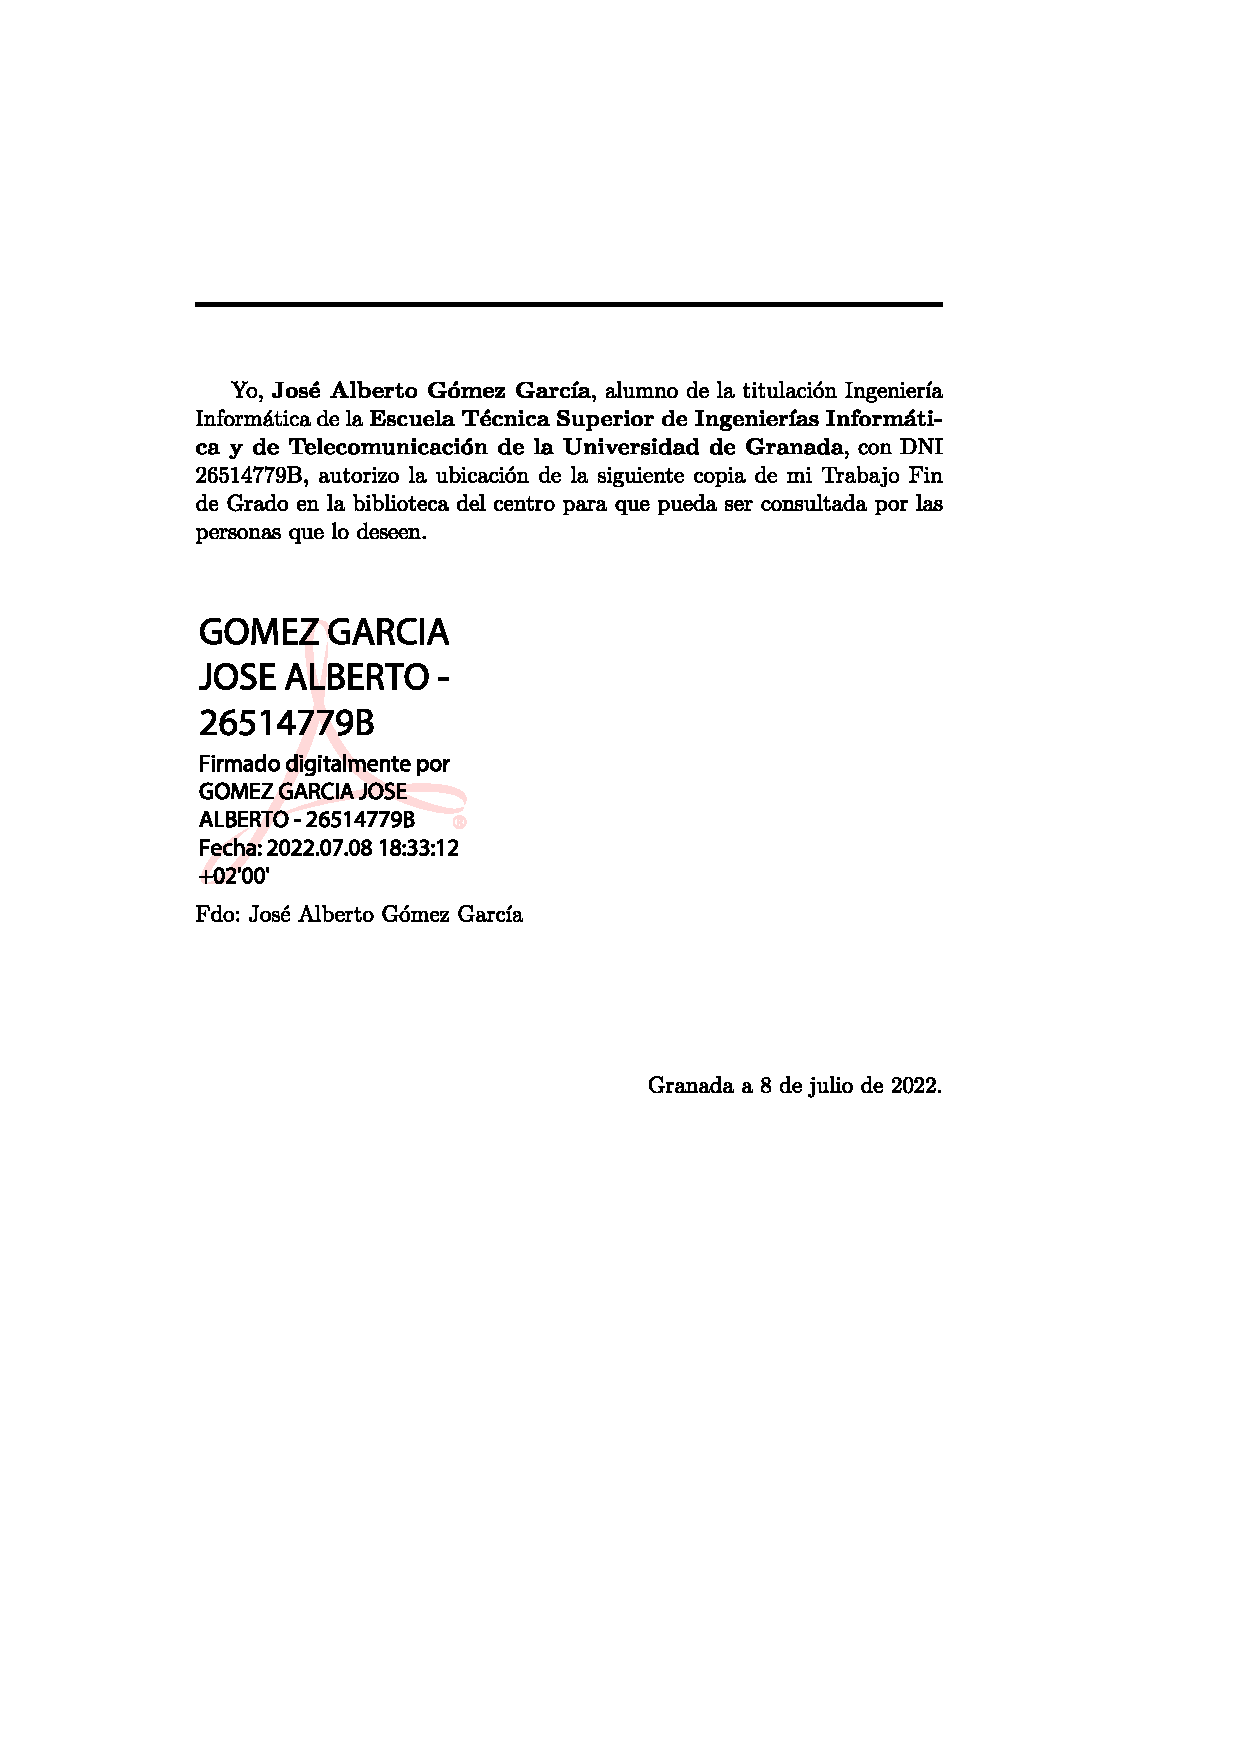
\includepdf[pages=-]{autorizo_biblioteca_ja_signed.pdf}
    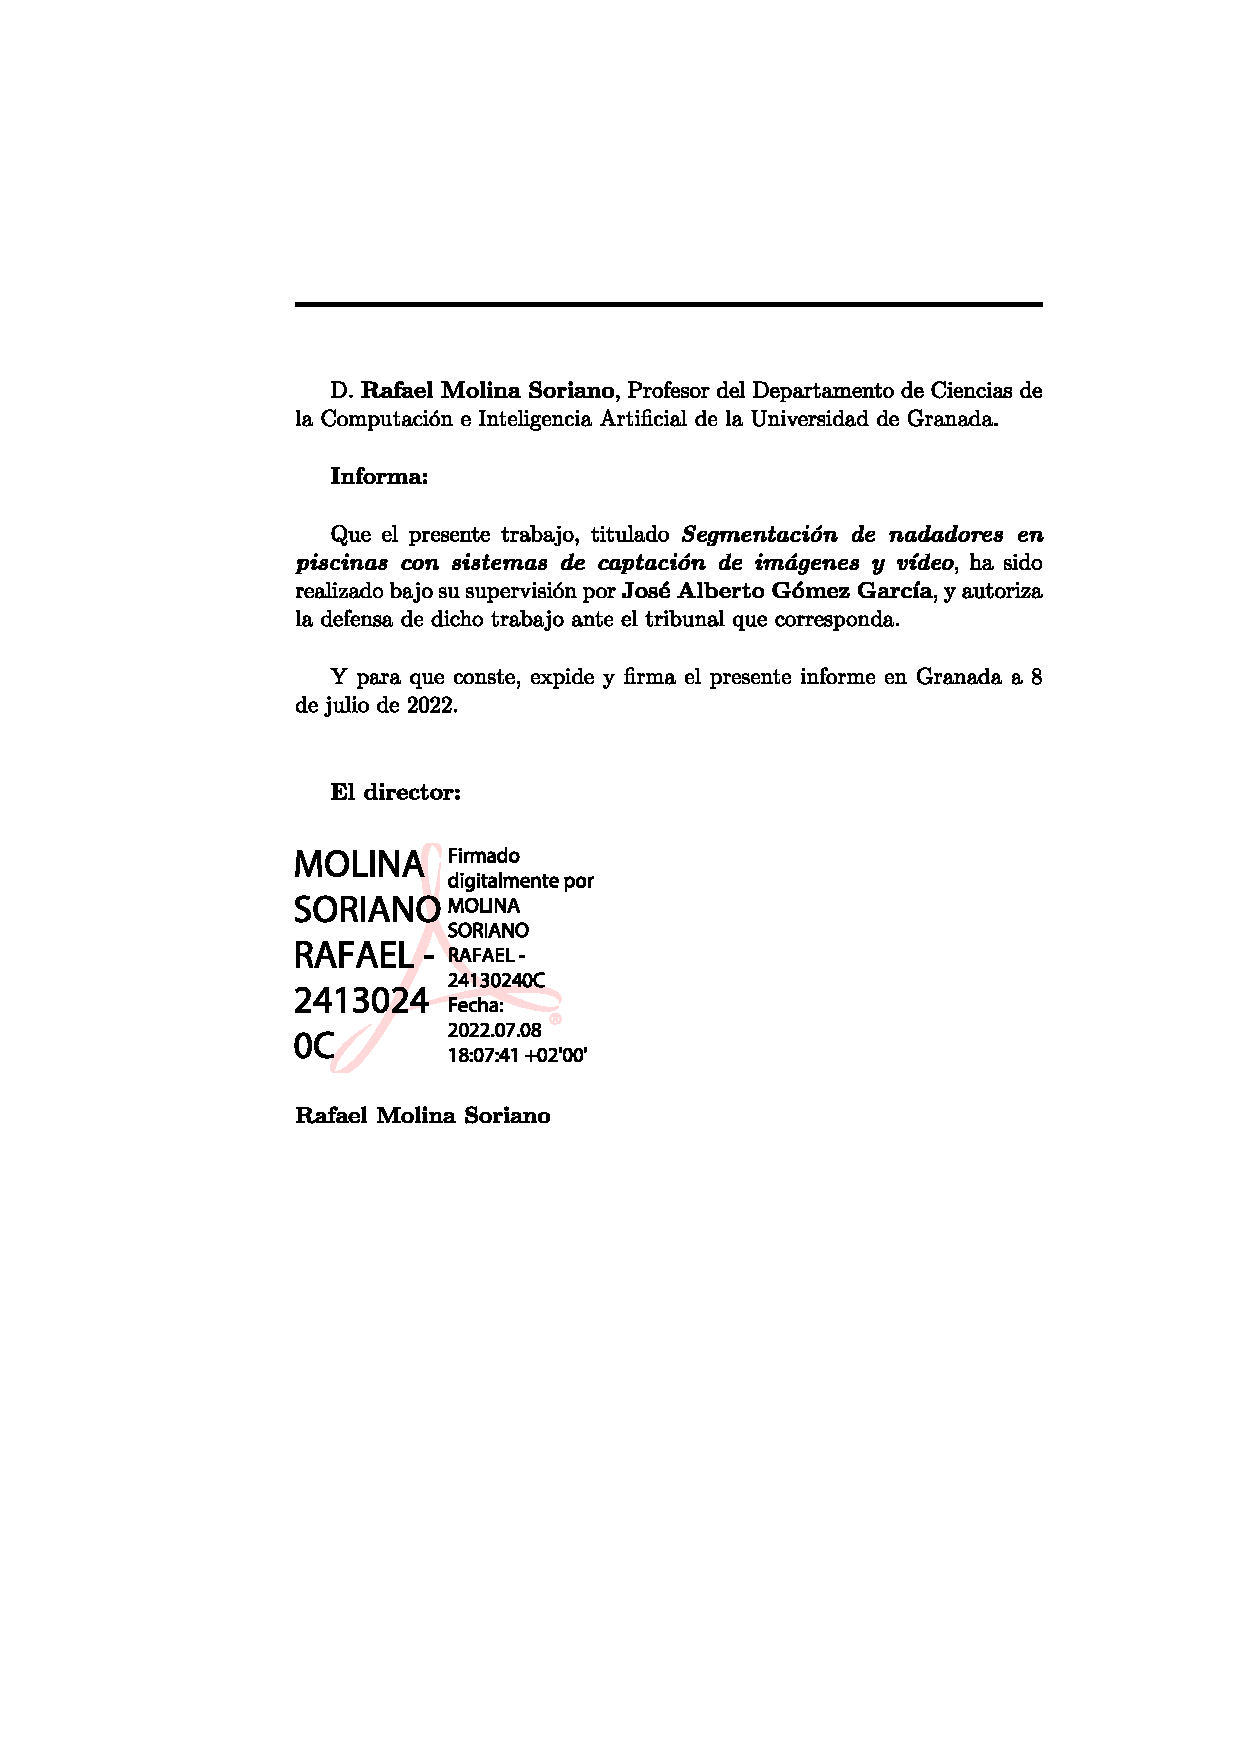
\includepdf[pages=-]{autorizo_rafa_defensa_signed.pdf}
	\newpage
	%\setcounter{tocdepth}{3}
	\tableofcontents
	

	% Índice de imágenes y tablas
	%\newpage
	\listoffigures

	% Si hay suficientes se incluirá dicho índice
	\listoftables 
	%\newpage

	%Introducción 
	\chapter{Introducción} \label{cap:capitulo1} 

La búsqueda de una forma física óptima mediante el entrenamiento deportivo ha tenido una gran importancia a lo largo de la historia del ser humano.
Ya en la antigüedad, durante la época helenística \cite{anta2013nuevas}, los atletas de élite que participaban en los juegos olímpicos se sometían a estrictos programas de entrenamiento, de un mínimo de diez meses de duración, y gozaban de un considerable reconocimiento social y económico. 

En 1896, con el resurgimiento de los juegos olímpicos modernos, los entrenadores se replantean los sistemas de entrenamientos a utilizar para alcanzar resultados óptimos \cite{anta2013nuevas}. Se pasa de un sistema de entrenamientos basado en el ensayo y error, a uno que busca técnicas y metodologías concretas que permitan maximizar las diferentes cualidades requeridas por los atletas de máximo nivel. Es a partir de este momento en el que la ciencia y la tecnología se ponen al servicio del deporte de élite con el objetivo de maximizar el rendimiento de los atletas.

Con el paso de los años, se introducen cada vez más sistemas cuyo objetivo es recabar información individual y personalizada para cada deportista. Hoy en día, tanto aficionados como profesionales, disponen de pulseras y relojes inteligentes que permiten medir el número de pasos andados, la velocidad a la que corremos, el esfuerzo realizado durante un partido de un tenis, la calidad de nuestro sueño, y otros muchos factores. Esta información proporciona una visión general sobre el desempeño deportivo y nuestra evolución conforme se entrena. 

Sin embargo, los deportistas de alto nivel requieren de sistemas más complejos que generen información concreta, detallada y específica para su ámbito deportivo. Por ejemplo, los velocistas emplean trajes especiales con multitud de sensores adheridos que permiten monitorizar el esfuerzo realizo por los músculos, la velocidad y aceleración del movimiento y demás parámetros, con los que se genera un modelo tridimensional del movimiento del deportista. A partir de la información generada, el entrenador puede sugerir rutinas de entrenamiento personalizadas que refuercen los puntos débiles del atleta, a la vez que se evitan lesiones \cite{rolecience}. También se emplean sistemas de realidad virtual \cite{sportvr} para aportar retroalimentación y entrenar correctamente la memoria gesticular, la cual resulta de especial importancia en deportes como el baloncesto, en los que movimientos rápidos y precisos son vitales.

Estos sistemas aportan una información de incalculable valor \cite{rolecience}. Consciente de esto, el profesor Raúl Arellano, catedrático de educación física de la Universidad de Granada especializado en natación, biomecánico, analista de la selección española de natación e investigador del grupo \textit{Aquatic Labs} de la UGR \cite{aquaticlabs}, ha utilizado multitud de sistemas de recogida de datos y ha analizado la influencia de diversos parámetros en el rendimiento de sus nadadores. 

En sus investigaciones \cite{raulvortice} \cite{raulonda} \cite{raulpropulsion},el profesor Raúl Arellano ha analizado, entre otros aspectos, la importancia del movimiento ondulatorio generado por el nadador en periodos subacuáticos y la correcta sincronización de las ondas generadas por brazo, tronco y piernas; ha caracterizado el vórtice generado en el agua por los mejores nadadores del mundo al introducirse en la piscina tras saltar del trampolín y ha intentado establecer correspondencias entre las fuerza generada por las piernas del nadador en el salto a la piscina y en la voltereta en la que se cambia el sentido del nado. Mediante este y otros trabajos busca perfeccionar los actuales métodos de entrenamiento y desarrollar nuevas metodologías que permitan maximizar el rendimiento de los deportistas a los que entrena. La importancia de su investigación trasciende el ámbito puramente científico y ha generado interés en la sociedad general, de hecho, su trabajo fue objeto de entrevista en la cadena de televisión andaluza Canal Sur en el año 2019. Esta puede ser visualizada en \cite{entrevistaraul}.

Con el objetivo de continuar su investigación, se ha desarrollado un modelo capaz de calcular la frecuencia media de nado de un nadador a partir de una secuencia de vídeo. En el presente trabajo detallaremos el proceso de desarrollo de la solución y su implementación. En el capítulo \ref{cap:capitulo2} describiremos el problema planteado con más detalle. En los capítulos siguientes, analizaremos y compararemos metodologías con las que detectar y rastrear al nadador durante su avance en la piscina. En concreto, en el capítulo \ref{cap:capitulo3} se analizan técnicas clásicas y en el capítulo \ref{cap:capitulo4} técnicas de aprendizaje profundo. Posteriormente, en el capítulo \ref{cap:capitulo5} analizaremos los datos recabados y ofreceremos un modelo del cálculo de la frecuencia media de nado. Finalmente, el capítulo \ref{cap:capitulo6} expondremos las conclusiones y discutiremos posibles lineas de trabajo futuro.
	\chapter{Descripción del problema} \label{cap:capitulo2}

El objetivo de este trabajo es plantear e implementar una solución que permita calcular la frecuencia media de nado de un nadador a partir de una secuencia de vídeo. En el presente capítulo se presentan los requisitos y detalles del problema, un análisis de los trabajos que ya se han llevado a cabo en este ámbito y una breve introducción del método propuesto. Finalmente, se detalla el sistema de captación con el que se han grabado los vídeos que utilizaremos.

Para comenzar, definimos la frecuencia media de nado como el número de brazadas que realiza un nadador por unidad de tiempo o el número de brazadas que han sido necesarias para avanzar una cierta distancia. A su vez, podríamos definir brazada como el movimiento enérgico que se hace extendiendo y recogiendo ambos brazos y que permite generar el impulso suficiente para que el nadador avance por el agua de la piscina.  

En las competiciones de natación, los diferentes nadadores deben recorrer un determinado número de veces el largo de la piscina, el cual suele recibir el nombre de ``split''. La piscina de la Facultad de Ciencias del Deporte de la UGR tiene un largo de 25 metros, al ser una piscina semi-olímpica. 

Queremos calcular el número de brazadas que un determinado nadador realiza en cada uno de los splits. Para ello, se nos indica que deberemos despreciar la distancia recorrida gracias al salto del nadador desde el trampolín y la voltereta con la que se cambia el sentido del nado. Estos instantes no son de interés dado que el nadador no bracea de forma continuas, si no que utiliza el impulso del salto y la propulsión con la pared, respectivamente. También queremos calcular el número de brazadas por minuto a lo largo de toda la prueba, con las mismas consideraciones que se acaban de mencionar.

\section{Trabajos relacionados}

La especificación de sistemas que calculen de forma automática la frecuencia de nado ya ha sido abordada en el pasado. Sin embargo, la mayoría de artículos consultados, como \cite{swimmerautostrokeratio}, hacen uso de sensores adheridos al cuerpo o traje de baño del nadador con tal fin, en lugar de secuencias de vídeo.

Aquellos trabajos que hacen uso de secuencias de vídeo se centran en la detección del nadador, y valoran el uso de diversas técnicas con dicho fin.

Trabajos como \cite{swimmerarti} proponen el uso del espacio de color HSV (Hue, Saturation, Value) y el uso del algoritmo de sustracción de fondos MOG (Mixture of Gaussians) para diferenciar zonas en movimiento de zonas estáticas. Posteriormente, se utiliza el método \textit{Mean Shift Clustering} para delimitar el contorno del nadador. Estos datos se utilizan para entrenar a un detector capaz de seguir el movimiento del nadador a lo largo de la piscina. En el artículo se hace especial hincapié en la dificultad de la detección del nadador debido a los cambios en el ambiente que produce el chapoteo en el agua y los reflejos en el agua de las fuentes de luz.

Otras investigaciones, como \cite{swimmerartii}, prestan especial atención a la influencia del espacio de color utilizado. Tras analizar el rendimiento del método de Yoon \cite{yoonmethod} sobre el espacio de color RGB (Red, Green, Blue) y la aplicación del algoritmo MOG sobre la representación HSV, como en \cite{swimmerarti}, el autor propone un método para detectar nadadores basado en las diferencias de los valores de las bandas de crominancia del espacio de color YCbCr.

En otros artículos se deja de lado el uso de técnicas clásicas del procesamiento de imágenes y se propone el uso de redes neuronales para detectar a los nadadores. Trabajos como \cite{swimmerartiv} utilizan redes neuronales para distinguir si el nadador está saltando desde el trampolín, nadando, buceando, o cambiado el sentido del nado. Otros, como \cite{swimmerartvi}, utilizan la inteligencia artificial para detectar las distintas posiciones en las que se puede encontrar un nadador durante una carrera. A partir de la sucesión de estas etapas se calcula la frecuencia de nado. En \cite{swimmerartiii} se discute el rendimiento de diversos tipos de redes neuronales convolucionales entrenadas para distinguir si un nadador está realizando una brazada o no. La frecuencia de nado se calcula a partir del número de detecciones que realice la red neuronal por unidad de tiempo. 

Cabe mencionar que también existen investigaciones \cite{swimmerartv} que utilizan técnicas de procesamiento de histogramas para detectar al nadador y seguir su movimiento.

La mayoría de trabajos consultados se centran solamente en la detección del nadador, o en la identificación de las diversas etapas por las que pasa un nadador en una carrera, sin calcular su frecuencia media de nado, objetivo último de este trabajo. Solamente \cite{swimmerartiii} y \cite{swimmerartvi} prestan atención a este aspecto. Como mencionamos anteriormente, en \cite{swimmerartvi} se utiliza la sucesión entre las etapas que conlleva una brazada, detectadas por una red neuronal, para calcular cuando el nadador está braceando y por consiguiente su frecuencia de nado, mientras que en \cite{swimmerartiii} se utiliza las detecciones de una red neuronal entrenada para detectar momentos en los que el nadador se encuentra realizando la brazada para posteriormente calcular la frecuencia de nado.

También cabe mencionar que existen compañías que ofrecen sistemas de cámaras y paquetes software, como \textit{\href{https://www.swimmingcam.com/}{Swimpro}} y \textit{\href{https://www.dartfish.com/swimming}{Dartfish}}, con los que obtener diversas métricas sobre el rendimiento de los nadadores, entre las que se encuentran la frecuencia media de nado. Sin embargo, y como era de esperar, estas compañías no ofrecen información alguna sobre cómo realizan sus cálculos.

Dado que el material del que partimos es significativamente diferente al usado por la mayoría de artículos, proponemos un modelo propio para calcular la frecuencia media de nado. 

\section{Método propuesto}

El método que proponemos en este trabajo tiene dos pasos diferenciados: (i) detección del nadador y (ii) estimación de brazadas.

En primer lugar, necesitamos poder reconocer al nadador durante la prueba y estimar la posición de la piscina en la que se encuentra. Tras haber consultado los trabajos previos expuestos anteriormente, decidimos abordar (i) desde dos puntos de vista distintos.

En el capítulo \ref{cap:capitulo3} se propondrá un modelo basado en técnicas clásicas del procesamiento de imágenes. Este buscará distinguir elementos estáticos y dinámicos, y, una vez reconocidos los elementos dinámicos, extraerá el contorno del nadador. En el capítulo \ref{cap:capitulo4} se propondrá un modelo basado en técnicas de aprendizaje profundo para reconocer y ubicar al nadador. 

En la figura \ref{fig:primerejemplodeteccion} se puede apreciar cómo estos métodos nos devuelven una caja que contiene al nadador. Esta nos proporcionará los datos que utilizaremos para el segundo paso: estimar el número de brazadas y calcular la frecuencia media de nado. 

\begin{figure}
    \centering
    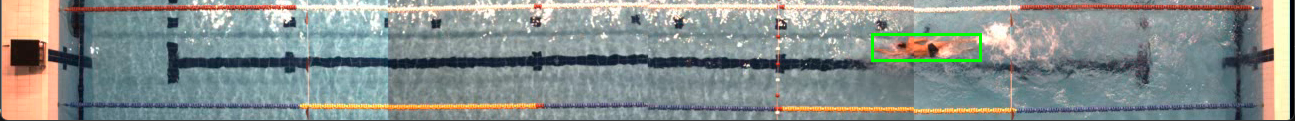
\includegraphics[width=\textwidth,height=\textheight,keepaspectratio]{imagenes/capitulo2/ejemplo_bbox.png}
    \caption{Ejemplo de detección de un nadador.}
    \label{fig:primerejemplodeteccion}
\end{figure}

En la figura \ref{fig:primerejemplovariacionanchura} se puede observar cómo varía la anchura de la caja que contiene al nadador. Dado que el movimiento del nadador tiene un carácter periódico, podemos estimar el número de brazadas (ii) a partir de la variación en la anchura de la caja. Podemos considerar que la brazada se completa en producen en momentos de máxima anchura, ya que el nadador debe extender los brazos. De esta forma, podemos detectar las brazadas de una manera sencilla identificando los máximos de la función.

\begin{figure}[h!]
    \centering
    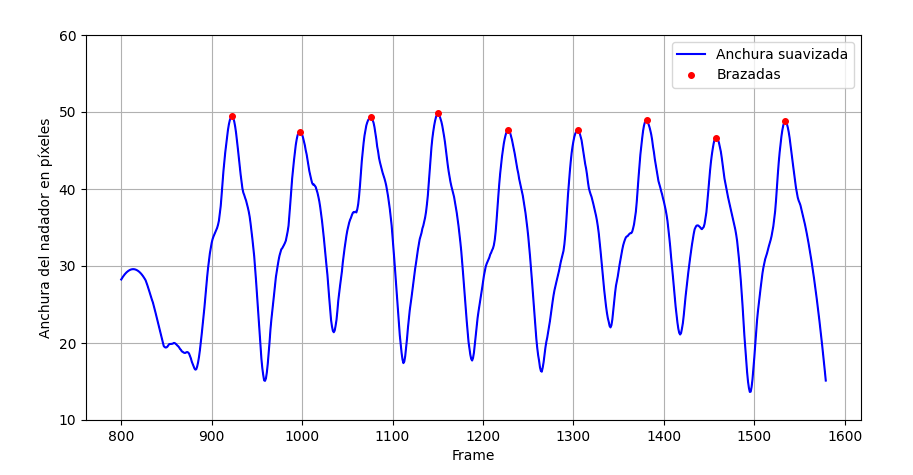
\includegraphics[width=\textwidth,height=\textheight,keepaspectratio]{imagenes/capitulo2/ejemplo_variacion_altura.png}
    \caption{Variación de anchura de la caja que contiene al nadador.}
    \label{fig:primerejemplovariacionanchura}
\end{figure}

Para calcular el tiempo que el nadador tarda en completar un tramo de 25 metros, podemos usar la variación en las coordenadas X de la caja. Estos valores pasarán de tener una tendencia creciente a decreciente, o viceversa, cuando se cambie el sentido del nado. En la figura \ref{fig:primerejemplovariacionsentido} se puede apreciar este hecho. Conocido el número de fotogramas en los que se mantiene cada una de las tendencias, y la tasa de fotogramas por segundo del vídeo, se puede calcular fácilmente el tiempo que se tarda en recorrer cada split.

\begin{figure}[h!]
    \centering
    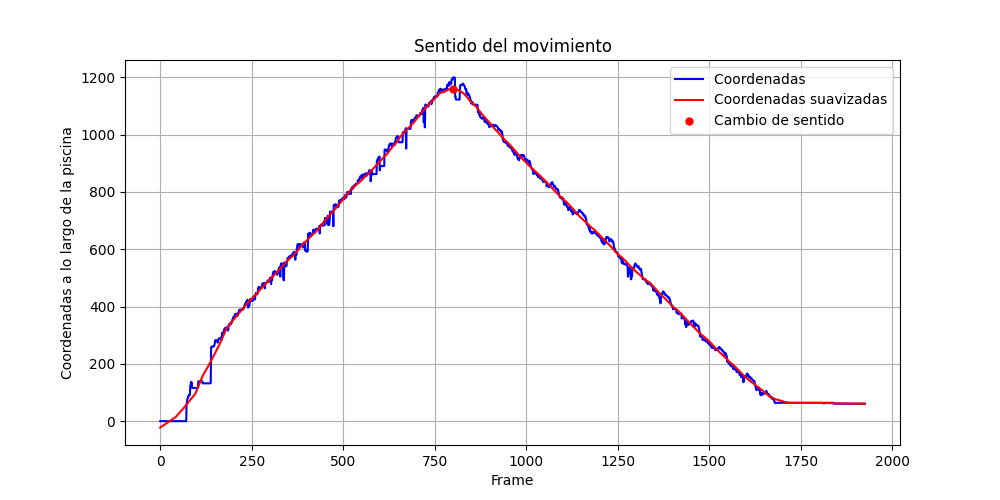
\includegraphics[width=\textwidth,height=\textheight,keepaspectratio]{imagenes/capitulo2/ejemplo_cambio_sentido.png}
    \caption{Variación en las coordenadas X de la caja que contiene al nadador.}
    \label{fig:primerejemplovariacionsentido}
\end{figure}

Estos cálculos, así como consideraciones adicionales a tener en cuenta, se discutirán a lo largo del capítulo \ref{cap:capitulo5}.

\section{Sistema de captación de vídeo}

El presente trabajo se ha diseñado y probado con grabaciones cenitales de los entrenamientos y competiciones que se realizan en las instalaciones de la UGR. Dada su importancia, analizaremos cómo se generan estos vídeos.

En el techo del pabellón en el que se encuentra la piscina de la Facultad de Ciencias del Deporte de la UGR podemos encontrar un sistema de 8 cámaras IP. Estas cámaras se sincronizan mediante software, generando un único vídeo en el que se puede visualizar la piscina completa.

El vídeo es generado mediante \textit{video stitching} \cite{LYU201955}. Esta técnica nos permite generar un único fotograma a partir de las zonas comunes, y que se suelen superponer, de los fotogramas generados por cada una de las cámaras del sistema. De esta manera, podemos obtener una imagen con mayor campo de visión. 

En la figura \ref{fig:pisicinaprimerjemeplo} mostramos un fotograma captado por el sistema de cámaras haciendo uso de esta técnica. En dicho fotograma podemos apreciar la diferencia de iluminación de la parte central de la piscina respecto de los extremos, o el desdoblamiento de la corchera en el centro de la piscina en dos. Estos serán aspectos que tendremos que tener en cuenta durante el desarrollo del trabajo.

\begin{figure}
    \centering
    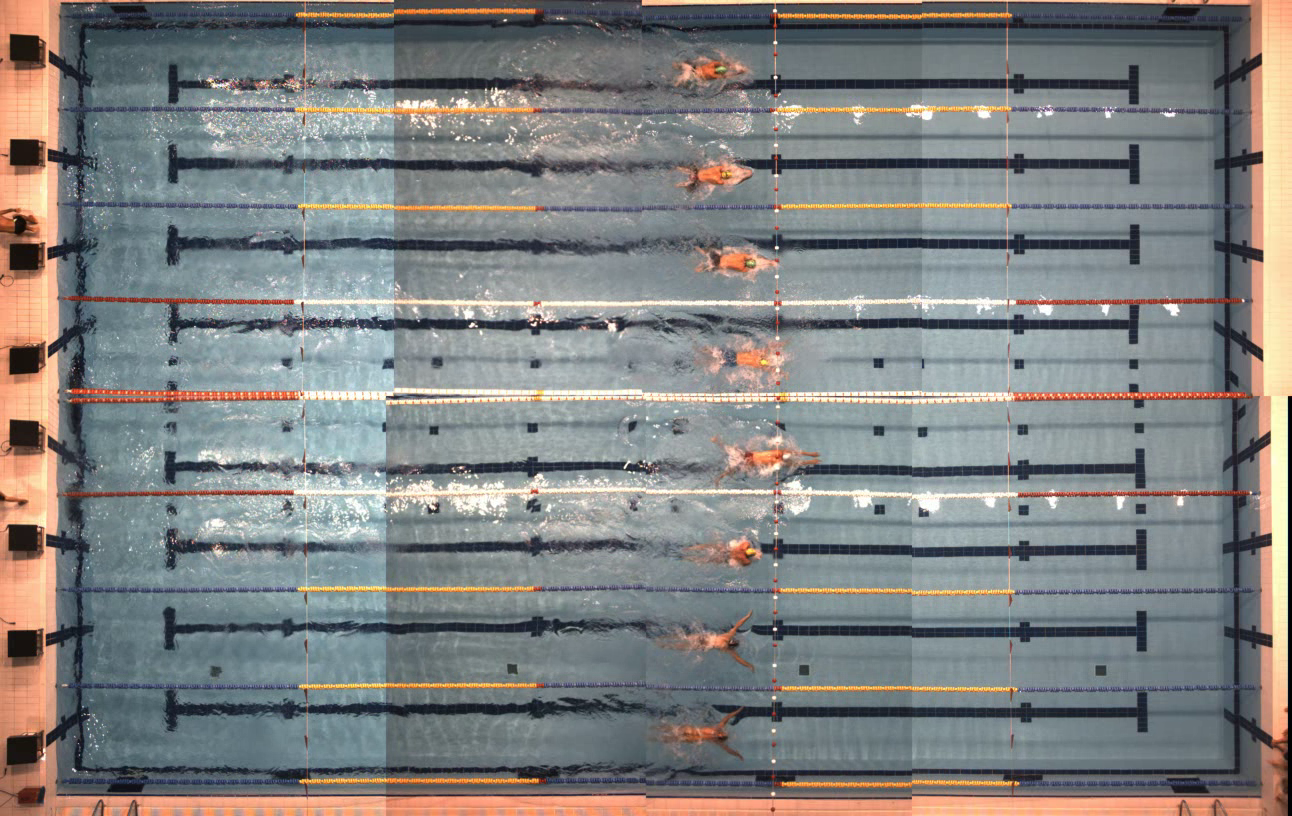
\includegraphics[width=\textwidth,height=\textheight,keepaspectratio]{imagenes/parte_BS/piscina_completa.png}    
    \caption{Fotograma captado por la matriz de cámaras.}
    \label{fig:pisicinaprimerjemeplo}
\end{figure}

Para controlar los parámetros del vídeo generado, tales como resolución y número de fotogramas por segundo, se utiliza el programa \textit{\href{https://www.baslerweb.com/en/products/basler-pylon-camera-software-suite/pylon-viewer/]}{Pylon Viewer}}, el cual también permite capturar imágenes de cada una de las cámaras por separado. La matriz de cámaras instaladas en el pabellón permite grabar a una resolución máxima de 2584x1632 píxeles y una tasa máxima de 83.33 fotogramas por segundo. Sin embargo, normalmente se utiliza una resolución de 1292x816 y una tasa de 41.66 fotogramas por segundo. 

Ahora que se conoce el problema y las características de los vídeos que se utilizarán, se procederá a explicar en detalle cómo se ha llevado a cabo la detección del nadador en los capítulos \ref{cap:capitulo3} y \ref{cap:capitulo4}. El calculo de la frecuencia de nado, a partir de la estimación de las brazadas realizadas por el nadador, se detallará en el capítulo \ref{cap:capitulo5}.


	\chapter{Detección de nadadores mediante técnicas clásicas } \label{cap:capitulo3}

En este capítulo abordaremos la detección del nadador en la piscina mediante técnicas clásicas del procesamiento de imágenes, separando el problema en tres apartados. En primer lugar, trataremos la importancia de una correcta selección del espacio de color sobre el que trabajar. Como segundo paso abordaremos la sustracción de fondos para distinguir los elementos estáticos de los dinámicos. Por último, obtendremos las bounding boxes que contienen al nadador. La sección concluye con una evaluación experimental que compara las distintas aproximaciones.

\section{Espacios de color}

Una de las primeras decisiones que debemos tomar cuando tenemos que procesar una imagen es el espacio de color en el que vamos a representar la información.

Las fotografía o vídeos que visualizamos diariamente, mediante la multitud de pantallas que nos rodean continuamente, suelen utilizar el espacio de color RGB, pero este no es el único modelo de color en que podemos representar nuestras imágenes; existen otras alternativas como HSV e YCbCr. A continuación, vamos a comentar las características de cada uno de estos tres espacios de color y su posible utilidad en nuestro problema. La elección de estos tres espacios de color concretos, RGB, HSV e YCbCr, viene motivada por su uso en publicaciones anteriores, tales como \cite{swimmerarti} y \cite{swimmerartii}. Nótese que este trabajo no pretende ser una revisión exhaustiva de los modelos de color y tan solo se recogen los que van a ser utilizados.

\subsection{RGB}

El espacio de color RGB es un espacio de color aditivo, en el que cada posible color se representa mediante la mezcla por adición de otros colores base \cite{abitofallcolorspaces}. En concreto, se utilizan los tres colores primarios aditivos; rojo (R), verde (G) y azul (B). Sin embargo, este modelo de color no define por sí mismo qué son los colores rojo, verde y azul, por lo que su representación puede diferir en función del dispositivo y del tipo de elemento físico que utilice cada uno de ellos para producir la luz, y por tanto, cada uno de los colores.

El esquema de representación del color RGB fue propuesto por primera vez en 1809 por el físico y oftalmólogo inglés Thomas Young. Según su trabajo en \cite{rgbtrivision}, la visión humana es tri-cromática dado que en la retina  disponemos de tres sensores para la percepción del color – los conos L, S y M -, siendo cada uno de ellos especialmente sensible a longitudes de onda diferentes, correspondientes a los colores primarios aditivos anteriormente mencionados. Una consecuencia de este hecho es que las representaciones de color sean también tri-cromáticas. Cuando los colores primarios se mezclan entre sí por parejas en la misma proporción aparecen los colores secundarios, el magenta, azul cian y amarillo. Para obtener el blanco mezclamos los tres colores primarios, mientras que para obtener el negro simplemente debemos no utilizar color alguno. Este sistema permite la definición y visualización de un gran número de colores, proporcional al número de bits que utilicemos para representar la cantidad de cada color primario. Por ejemplo, si utilizamos 8 bits para cada color primario podremos representar 16.777.216 colores.

Para representar el conjunto de colores RGB se suele emplear cubos como los que se muestran en la figura \ref{fig:cubosRGB}.

\begin{figure}[h!]
    \centering
    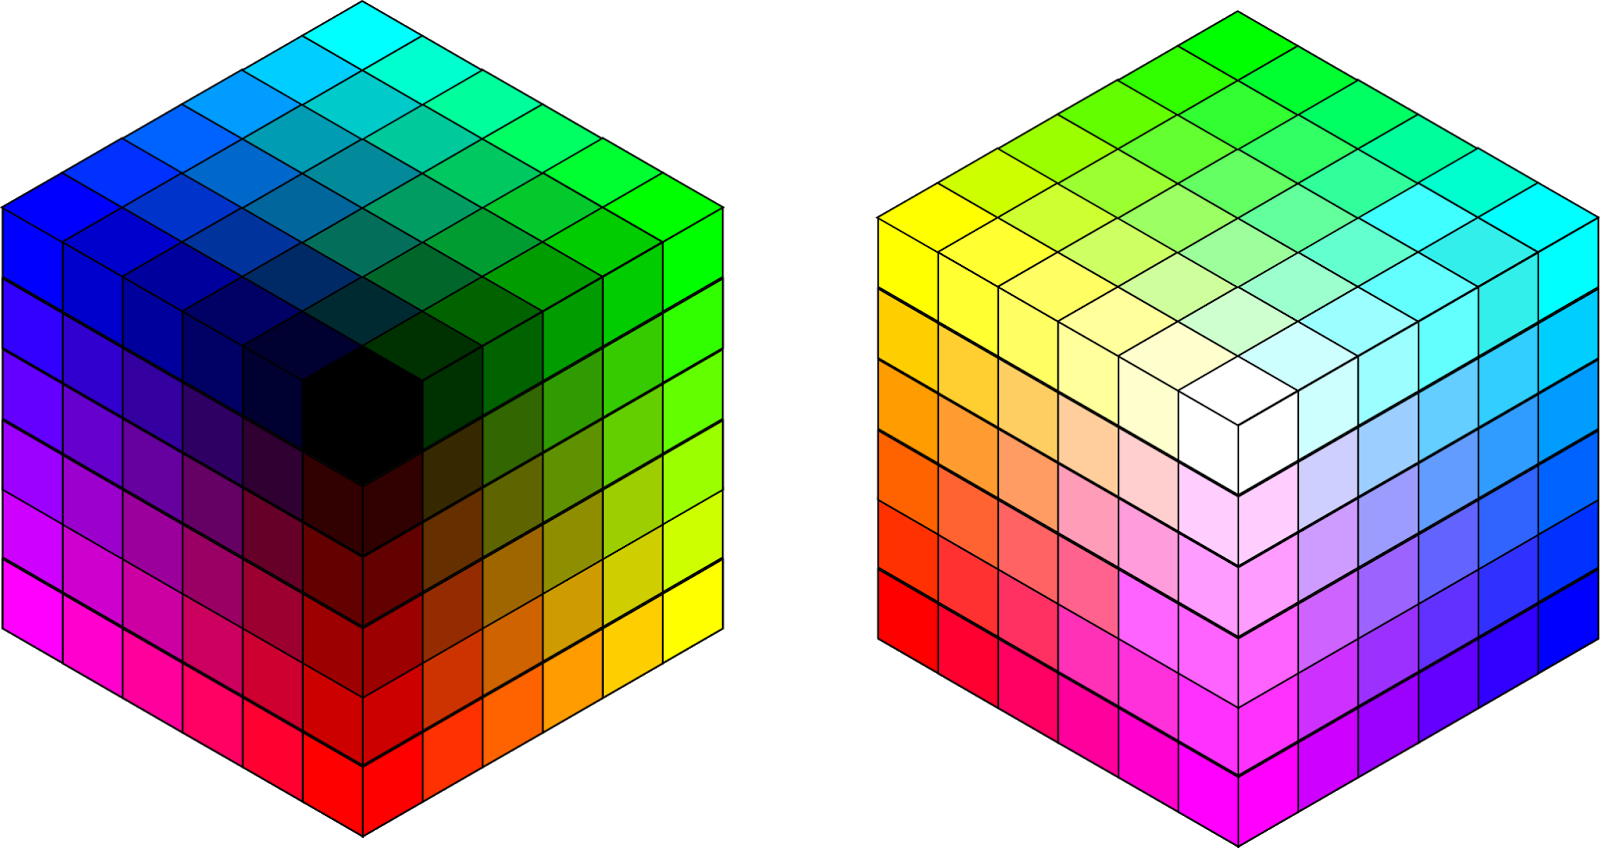
\includegraphics[width=0.7\textwidth,height=0.7\textheight,keepaspectratio]{imagenes/parte_BS/cubos_rgb.png}    
    \caption{Representación del espacio de color RGB.}
    \label{fig:cubosRGB}
\end{figure}

RGB es un modelo de color, es decir, es una representación matemática que describe cómo se combinan los colores primarios. Sin embargo, hay multitud de espacios de color RGB distintos, con diferentes parámetros, que han sido creados con el paso del tiempo ante la necesidad de los consumidores, intereses profesionales o avances tecnológicos. También existen multitud estándares que determinan que parámetros deben usarse en qué situaciones \cite{rgbtrivision}. Podemos mencionar los espacios \textit{sRGB}, \textit{AdobeRGB}, \textit{CIE 1931 RGB}, \textit{NTSC} y \textit{DCI-P3}; y los estándares \textit{SMPTE-C}, \textit{ITU-R BT.601} e \textit{ITU-R BT.709-3}.

\subsection{HSV}

El modelo de color HSV, creado por Alvy Ray Smith en 1978 \cite{abitofallcolorspaces}, tiene como principal objetivo representar con mayor exactitud la forma en la que la visión humana percibe los atributos que componen cada color.

Para representar los colores este modelo utiliza tres componentes, llamadas tono (hue), saturación (saturation) y valor (value). Pasemos a describir cada componente \cite{libroTID}.
\begin{itemize}
    \item El tono representa el atributo de una sensación visual según la cual un área parece similar al color rojo, amarillo, verde, azul o a una combinación de dos de los colores anteriores en respuesta a la longitud de onda de la luz captada. La gama cromática se suele representar en una rueda o cono circulares, como se puede apreciar en la figura \ref{fig:conoHSV}, de manera que se indica el color mediante un ángulo entre 0 y 360 grados. En particular, un ángulo de 0º corresponde al rojo, uno de 120º corresponde al verde y uno de 240º corresponde al azul.
    \item La saturación indica la cantidad de color que tenemos en un área en proporción a su brillo, es decir, su pureza; o dicho de otro modo, la cantidad de blanco que se encuentra embebida en un color concreto. Este valor se representa como un número entre 0 y 1, o un porcentaje entre 0 y 100.
    \item El valor representa el atributo de una sensación visual según el cual un área parece emitir más o menos luz. Una vez más, el valor se representa mediante un porcentaje entre 0 y 100 o un número entre 0 y 1.
\end{itemize}

\begin{figure}[h!]
    \centering
    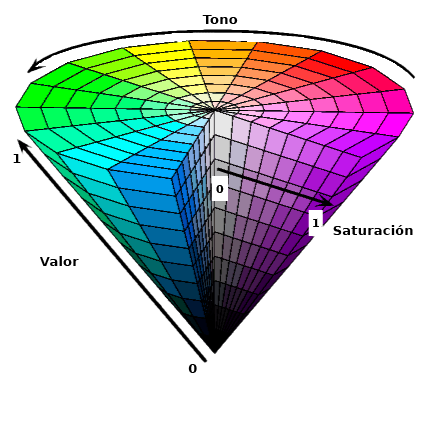
\includegraphics[width=0.5\textwidth,height=0.5\textheight,keepaspectratio]{imagenes/parte_BS/cono_hsv.png}    
    \caption{Representación del espacio de color HSV.}
    \label{fig:conoHSV}
\end{figure}

Existen otros modelos (HSI y HSL) que comparten los conceptos de tono y saturación y se consideran de la misma familia. No ocurre lo mismo con el concepto de valor, que se sustituye por intensidad y luminancia respectivamente. HSI y HSL no se utilizan en este trabajo, pero el lector interesado puede consultar las diferencias en \cite{abitofallcolorspaces}.

\subsection{YCbCr}

El modelo de color YCbCr es ampliamente usado para la representación de vídeo digital – especialmente en televisión - dado que forma parte de la recomendación \textit{ITU-R BT.601} de la \textit{ITU (International Telecommunication Union)} que se sigue en la Unión Europea \cite{abitofallcolorspaces}. 

Este modelo de color utiliza tres componentes, una de luminancia y dos de crominancia, para representar los colores.

\begin{itemize}
    \item Y: componente de luminancia que representa la intensidad del brillo del color. Por sí misma permite representar imágenes en blanco y negro.
    \item Cb: componente diferencial de crominancia azul, es decir, la diferencia entre luminancia y el valor azul.
    \item Cr: componente diferencial de crominancia roja. Representa la diferencia entre luminancia y el valor rojo. 
\end{itemize}

Según \cite{featureextraction}, el estándar obliga, para representaciones de 8 bits, a que el valor de la componente de luminancia esté comprendido entre los valores 16 y 235, mientras que los valores de las componentes de crominancia deben ser inferiores a 240. Esto se hace para que la conversión a RGB no produzca colores que dicho espacio de color no sea capaz de representar.

En la figura \ref{fig:planosycbcr} podemos observar la representación del plano Cb/Cr para diferentes valores de luminancia.

\begin{figure}[h!]
    \centering
    \begin{tabular}{ccc}
          
\includegraphics[width=0.28\textwidth,height=0.28\textheight,keepaspectratio]{imagenes/parte_BS/YCbCr_Y0.png} & 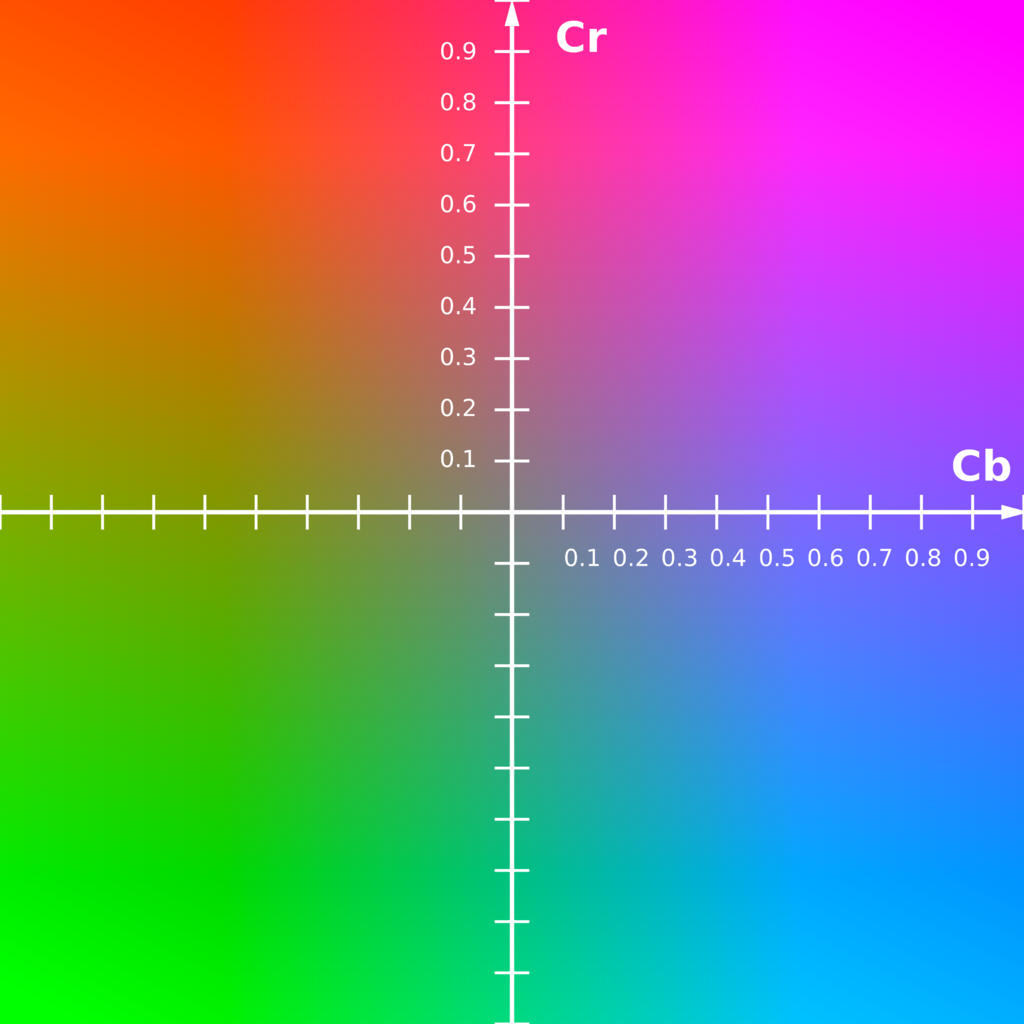
\includegraphics[width=0.28\textwidth,height=0.28\textheight,keepaspectratio]{imagenes/parte_BS/YCbCr_Y50.png} &
          
\includegraphics[width=0.28\textwidth,height=0.28\textheight,keepaspectratio]{imagenes/parte_BS/YCbCr_Y100.png} \\
          a) Y=0 & b) Y=0.5 & c) Y=1\\
     \end{tabular}
     \caption{Planos Cb/Cr para diferentes luminancias.}
     \label{fig:planosycbcr}
\end{figure}

En ocasiones, YCbCr e Y’CbCr se usan indistintamente, a pesar de ser modelos de color distintos \cite{moredigitalvideo}. En la versión con apóstrofo se utiliza corrección gamma, por lo que la componente de luminancia tendrá un valor en el rango [0, 1], mientras que las componentes de crominancia tendrán un valor en el intervalo [-0.5, 0.5]. A la hora de elegir un paquete software para tratamiento de imágenes deberemos tener en cuenta si permite el uso de ambos espacios de color, o en su defecto, cual de los dos se utiliza concretamente. Adicionalmente, tenemos que tener en cuenta que se suelen realizar conversiones de tal manera que los valores oscilen en el rango [0, 255].

En el modelo de color YCbCr se suele utilizar submuestreo de las componentes de crominancia \cite{submuestreocroma}. Codificando menos información de color que de luminancia, las imágenes ocupan menos espacio y su transmisión requiere un menor ancho de banda. Esta codificación no resulta en una degradación apreciable de la calidad de la imagen dado que el ojo humano es más sensible a la luminancia que al color \cite{submuestreocroma}.

Los diferentes formatos de submuestreo cromático se suelen representar mediante la notación X:Y:Z, donde X representa el tamaño de una región horizontal de muestreo - habitualmente de 4 píxeles - Y nos dice cuantas muestras para cada banda de crominancia se toman en una fila de largo X píxeles, y Z nos indica cuantos cambios en las muestras de crominancia hay entre la primera y segunda fila de X píxeles \cite{submuestreocroma}.

Los tres esquemas más utilizados son los siguientes:
\begin{itemize}
    \item 4:4:4. Para cada píxel muestreamos cada una de las componentes, por lo que no se produce compresión ni reducción de la calidad.
    \item 4:2:2. Para cada píxel muestreamos la componente de luminancia, pero las componentes de crominancia se muestrean para uno de cada dos píxeles horizontales.
    \item 4:2:0. Para cada píxel se muestrea la componente de luminancia, pero las componentes de crominancia se muestrean en un único píxel de una región 2x2 píxeles. 
\end{itemize}
Para un mejor entendimiento, en la figura \ref{fig:subsamplingycbcr} se puede apreciar el efecto de aplicar cada una de estas técnicas de submuestreo cromático. Cuanto menor sea el número de componentes de crominancia muestreadas, más similares serán los colores de una región 2x2 entre sí, a la vez que más diferentes de los colores originales.

\begin{figure}[h!]
    \centering
    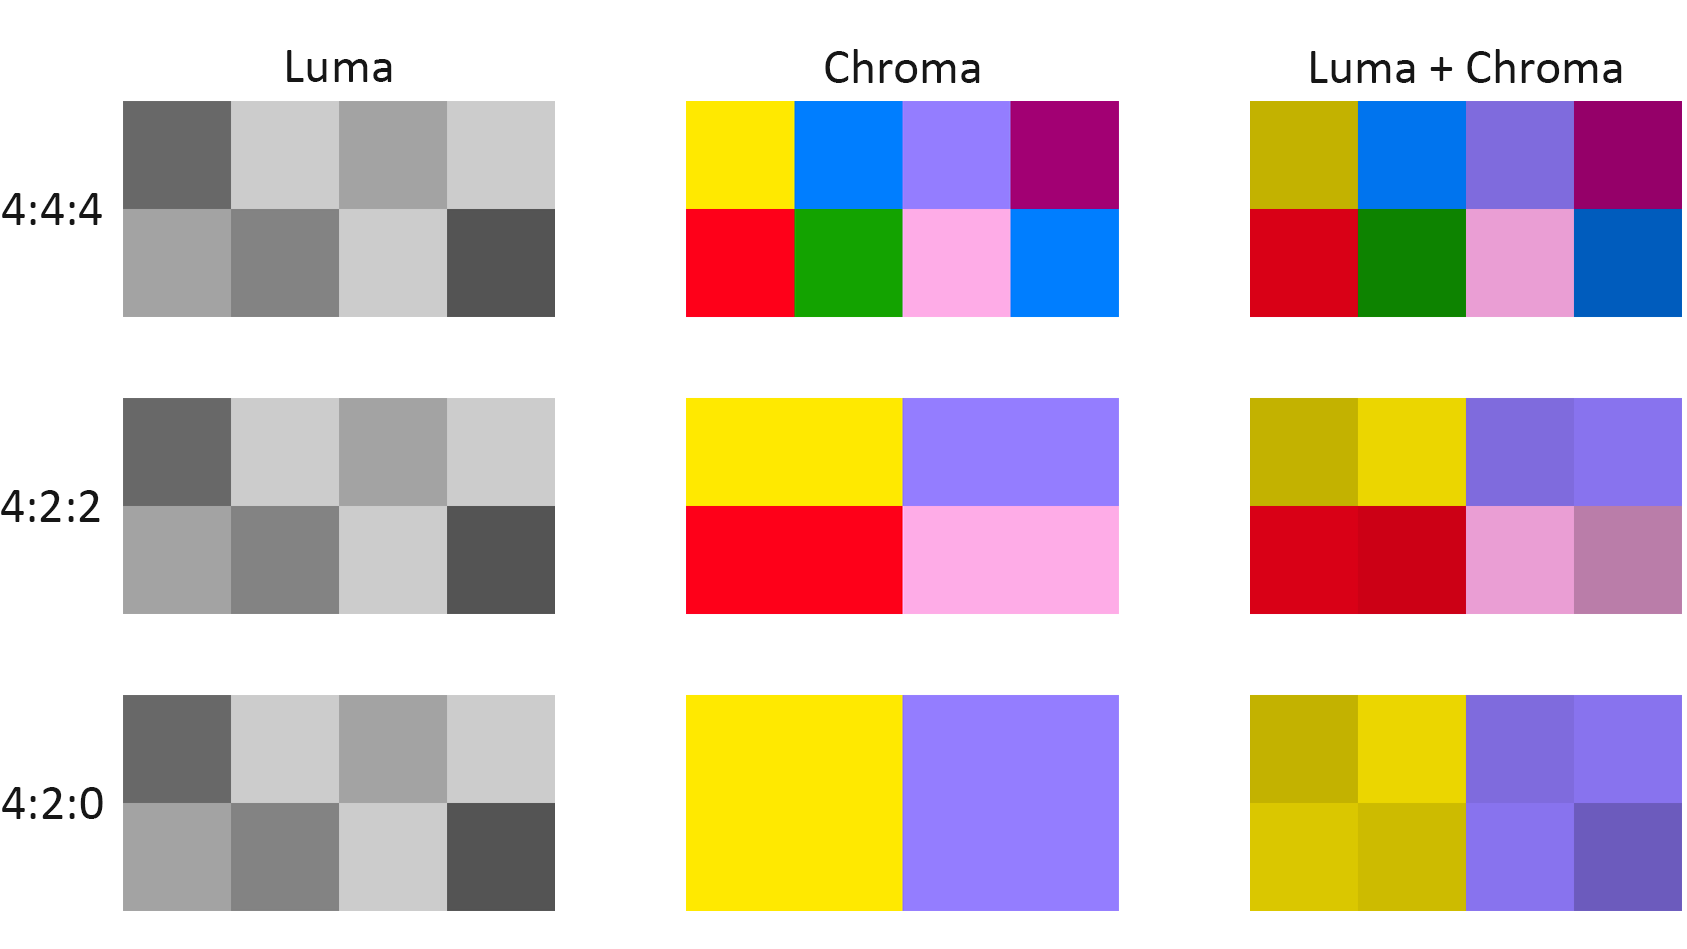
\includegraphics[width=0.65\textwidth,height=0.65\textheight,keepaspectratio]{imagenes/parte_BS/subsamplingycbcr.png}    
    \caption{Esquemas de submuestreo cromático.}
    \label{fig:subsamplingycbcr}
\end{figure}

\subsection{Elección del espacio de trabajo para la detección de nadadores y su justificación} \label{sub:elegirespaciocolor}

Una vez hemos comentado las características de los principales espacios de color, pasamos a analizar la posible utilidad de cada uno de ellos en nuestro problema concreto, la detección de nadadores. Realizamos este análisis dado que trabajos anteriores, como \cite{hsvforswimmerdetection}, \cite{swimmerartii}, \cite{footbalhsv} y \cite{swimmerdetectorii}, sugieren que la correcta elección del espacio de color influye significativamente en el rendimiento de los algoritmos de sustracción de fondos. 

En visión por computador es frecuente querer realizar filtrados en función del color; en nuestro caso querremos distinguir al nadador de una gran masa de agua de color principalmente azul. Así, podremos posteriormente facilitar el trabajo al algoritmo de sustracción de fondos.

Una primera aproximación a seguir es una variación del método de Yoon \cite{yoonmethod}, el cual utiliza la componente verde del espacio RGB para distinguir jugadores de fútbol en un campo de hierba principalmente verde. Artículos como \cite{swimmerartii} proponen usar la componente azul del espacio RGB para distinguir al nadador del agua de la piscina. Sin embargo, se llega a la conclusión de que este espacio de color no proporciona resultados óptimos. 

Esto es debido a los pequeños cambios de iluminación que puede haber en la imagen debidos al reflejo de los focos en el agua o el chapoteo generado por el avance del nadador. Estas situaciones modifican el color del agua, de manera que varían los valores de las tres componentes RGB, y no sólo la  componente azul, aunque nosotros percibamos visualmente que al agua sigue siendo azul \cite{swimmerartii}. Esto dificulta significativamente la tarea de filtrado. Además, debemos tener en cuenta que en la mayoría de los vídeos que nos han proporcionado los investigadores la parte central de la piscina tiene unas condiciones de iluminación significativamente distintas a las de los extremos. 

Como puede apreciarse en la figura \ref{fig:ejemplopiscinargb}, los valores de los distintos tonos de azul varían en función de la zona de la piscina. En las zonas extremos el agua es algo más oscura, que en los alrededores del primer y segundo tercio horizontal de la imagen, siendo significativamente más oscura el agua en la parte central de la piscina. Además, la línea central de adoquines de cada calle - conocida coloquialmente como T - tiene otro tono de azul mucho más oscuro que el del agua.

\begin{figure}[h!]
    \centering
    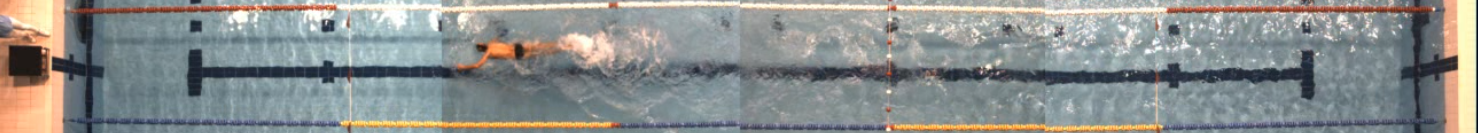
\includegraphics[width=1\textwidth,height=1\textheight,keepaspectratio]{imagenes/parte_BS/single_lane_RGB.png}   
    \caption{Calle de la piscina en espacio de color RGB.}
    \label{fig:ejemplopiscinargb}
\end{figure}

Si nos fijamos en la imagen \ref{fig:ejemplopiscinargbcanales}, donde mostramos por separado los canales RGB de un fotograma en el que sólo aparece una calle de la piscina, podremos apreciar que no existen grandes diferencias que nos permitan realizar el filtrado por el valor de uno solo de estos canales. Además, se mantienen los reflejos de los focos del pabellón sobre el agua en movimiento y el chapoteo que produce el nadador en todos los canales, lo cual podría ser considerado por el algoritmo de sustracción de fondos como movimiento, dificultando nuestra tarea.

\begin{figure}[h!]
    \centering
    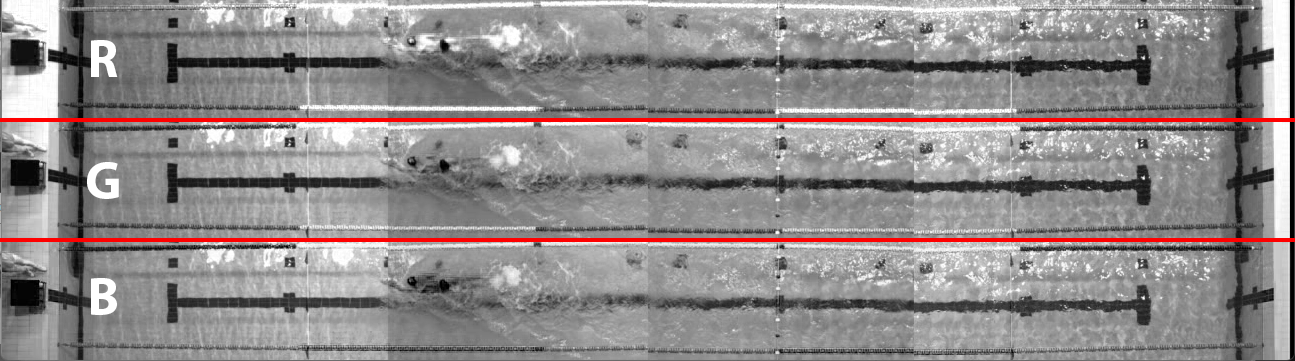
\includegraphics[width=1\textwidth,height=1\textheight,keepaspectratio]{imagenes/parte_BS/RGB_LANE.png}    
    \caption{Canales RGB por separado de una única calle de la piscina.}
    \label{fig:ejemplopiscinargbcanales}
\end{figure}

Por todos los inconvenientes expuestos, se descarta el uso el modelo de color RGB y se pasa a considerar otros modelos de color. 

En segundo lugar, consideremos el uso del espacio de color HSV. Trabajos como \cite{hsvforswimmerdetection}, \cite{pielespacioscolor} y \cite{swimmerartii} proponen el uso de este espacio de color dado que permite reducir la influencia de los cambios en la iluminación a la hora de realizar el filtrado deseado. Estos cambios, causados por reflejos en el agua, deberían quedar reflejados únicamente en las componentes de intensidad de la imagen, sin alterar la componente cromática, lo que facilita nuestra tarea de filtrado de colores. 

En la figura \ref{fig:ejemplopiscinahsvcanales} podemos apreciar el mismo fotograma que en la figura \ref{fig:ejemplopiscinargbcanales}. En esta ocasión, se muestran cada uno de los canales de la representación en el espacio de color HSV. 

\begin{figure}[h!]
    \centering
    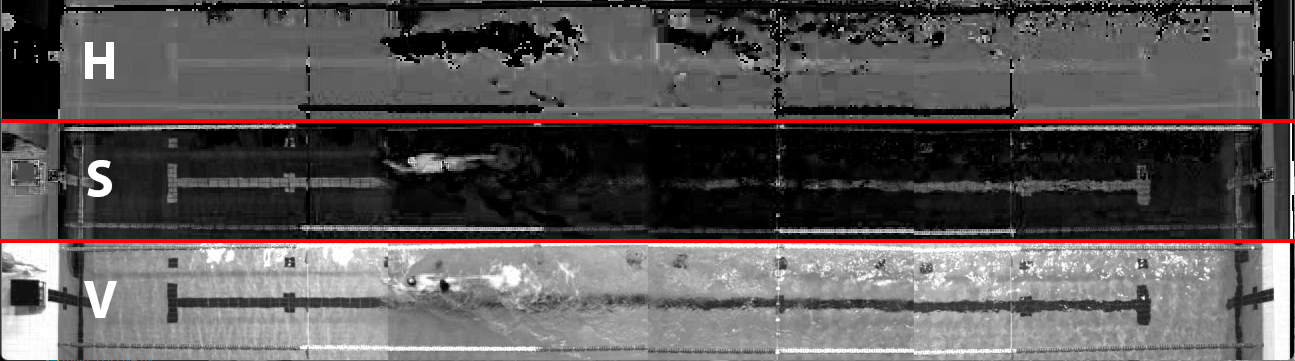
\includegraphics[width=1\textwidth,height=1\textheight,keepaspectratio]{imagenes/parte_BS/HSV_LANE.png}    
    \caption{Canales HSV de una calle de la piscina.}
    \label{fig:ejemplopiscinahsvcanales}
\end{figure}

Salta a la vista rápidamente que el canal de saturación  permite distinguir fácilmente al nadador, en colores cercanos al blanco, del resto de la escena. El agua adopta tonos oscuros, mientras que los azulejos azules del fondo de la piscina toman valores claros. Llegamos a conclusiones similares a las expuestas por los artículos anteriormente mencionados. 

Otras investigaciones, como \cite{ycbcrskini} \cite{skinvariousspaces} \cite{swimmerartii} abogan por el uso de las bandas de crominancia del espacio de color YCbCr para detectar la piel del individuo. En particular, \cite{ycbcrskini} utiliza la información de dichas bandas para calcular la cantidad de piel a la vista y decidir si una imagen es explícita o no. Nuestro objetivo final es distinto, pero compartimos similitudes con este enfoque dado que el nadador también deja gran cantidad de piel a la vista que podemos usar para diferenciarlo respecto del agua de la piscina.

En la figura \ref{fig:ejemplopiscinaycbcrcanales} podemos observar la misma situación que en figuras anteriores, pero con la diferencia de que la representación se hace por medio del espacio de color YCbCr. 

\begin{figure}[h!]
    \centering
    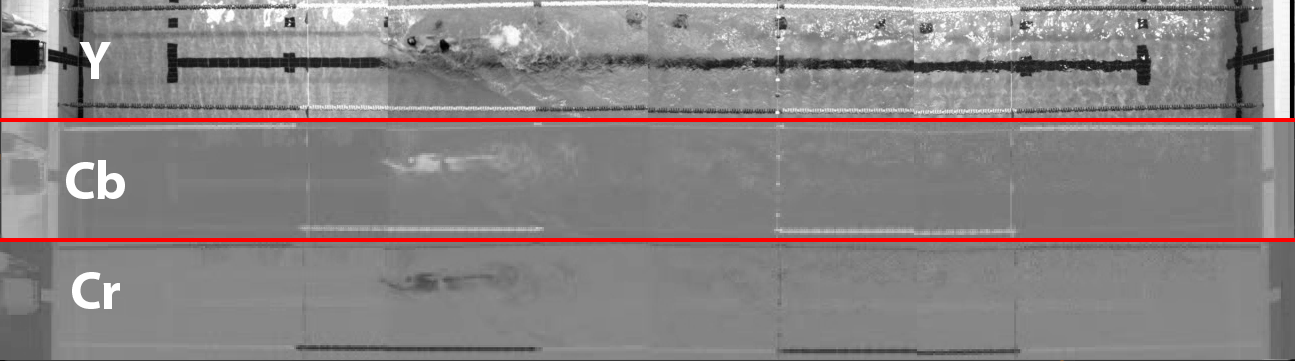
\includegraphics[width=1\textwidth,height=1\textheight,keepaspectratio]{imagenes/parte_BS/YCBCR_LANE.png}
    \caption{Canales YCbCr de una calle de la piscina.}
    \label{fig:ejemplopiscinaycbcrcanales}
\end{figure}

Si nos fijamos en las bandas de crominancia, Cb y Cr, podemos observar como el nadador es fácilmente distinguible del agua de la piscina, la cual se encuentra representada de forma bastante homogénea en un pequeño rango de colores. También podemos apreciar como no existen prácticamente reflejos en el agua proveniente de los focos del pabellón, y una menor cantidad de chapoteo que en la banda de luminancia Y. En \cite{swimmerartii} se llegan a estas mismas conclusiones, y proponen un método de detección de nadadores en función de la información que proporcionan las bandas de crominancia del espacio YCbCr.

A partir de lo mostrado en este apartado, podemos concluir que la banda de saturación del espacio HSV, y la bandas de crominancia del espacio YCbCr resultan especialmente prometedoras al permitir identificar de manera sencilla al nadador. Nuestras observaciones coinciden con la de trabajos previos como \cite{hsvforswimmerdetection} y \cite{swimmerartii}.

Evaluar experimentalmente cual de estas bandas es la más apropiada requiere de la extracción del contorno del nadador, que se discute en el apartado siguiente. Por ello, hemos pospuesto el análisis experimental a la sección \ref{sub:eleccionalgoritmo}.

\section{Sustracción de fondos} 

La sustracción de fondos es una técnica clásica del procesamiento de imágenes que permite detectar movimiento a partir de una secuencia de fotogramas capturados por una cámara estática. En su vertiente más básica, buscaremos detectar las diferencias entre el fotograma actual y el fotograma anterior, de manera que aquellos píxeles que no varíen serán considerados parte del fondo de la imagen – zonas estáticas - mientras que los píxeles cuyo valor haya sufrido cambios serán considerados parte de objetos en movimiento – zonas dinámicas. En las siguientes secciones trataremos de forma teórica los algoritmos de sustracción de fondos más populares.

\subsection{Mezcla de gaussianas}

El algoritmo de sustracción de fondos mediante “mezcla de gaussianas”, de siglas MOG, fue propuesto en el artículo \cite{origenmog}. Este método utiliza entre 3 y 5 distribuciones gaussianas de diferente media para modelar los valores en cada píxel de la imagen. Los autores de este algoritmo suponen que las diferentes distribuciones representan cada uno de los colores del fondo y primer plano de la imagen. Cada gaussiana tiene un peso asignado, el cual se va actualizando dinámicamente de forma que sea proporcional a la cantidad de tiempo que un píxel se mantiene con un determinado color. Cuando el peso de la distribución es pequeño se entiende que ese píxel cambia frecuentemente de valor, por lo que consideramos que forma parte del primer plano de la imagen.

La principal desventaja de este algoritmo es el número fijo y poco variable de distribuciones gaussianas a utilizar \cite{infomog}. Para solventar este problema se desarrolló una segunda versión del algoritmo \cite{mejoramog}, de siglas MOG2, que permite usar un número variable de distribuciones gaussianas para cada píxel en diferentes fotogramas. Al permitir una mejor representación de los colores de los píxeles, MOG2 proporciona un mejor rendimiento que la versión original del algoritmo, MOG. 

Cada implementación concreta de este algoritmo asigna un número de fotogramas previos que tener en cuenta para calcular el peso de cada distribución gaussiana durante el proceso de detección. 

\subsection{Vecinos más próximos}

En el artículo \cite{origenknn} se presenta una mejora del algoritmo basado en mezcla de gaussianas presentado en la sección anterior. Los autores utilizan ecuaciones recursivas para actualizar constantemente los parámetros de los modelos gaussianos y seleccionar el número apropiado de componentes para cada píxel. Además, se introduce el uso del algoritmo KNN para mejorar la estimación de la densidad del núcleo de las distribuciones gaussianas. 

Es esta versión mejorada del algoritmo MOG la que se conoce como algoritmo de sustracción de fondos K-NN (K vecinos más próximos) y se implementa en el paquete \textit{OpenCV}.

El algoritmo K-NN permite, a partir de un conjunto de datos etiquetados, definir un modelo de predicción con el que asignar valores de salida a datos nuevos.

Este algoritmo compara el argumento de entrada con todos los ejemplos disponibles antes de realizar una predicción. La comparación entre datos se realiza utilizando una función matemática que permita representar distancias - siendo las más comunes la distancia euclídea y la distancia de Manhattan.

Una vez se realizan las comparaciones entre datos, se tienen en consideración las K muestras más cercanas - con menor valor de distancia. Resulta de vital importancia elegir un valor del parámetro K adecuado al problema a resolver.

\subsection{Google Summer Of Code}

Vladislav Samsonov, bajo la mentoría de Maksim Shabunin, trabajó en la mejora de los algoritmos de sustracción de fondos del paquete software OpenCV durante el programa de formación \textit{Google Summer of Code} del año 2017 \cite{gsocprojectentry}. A pesar de que la propuesta inicial era la mejora del algoritmo LSBP descrito en \cite{originallbspgsoc}, su trabajo supuso además la implementación de un nuevo algoritmo para la eliminación de fondos, el cual ha recibido como nombre las siglas de dicho programa de formación, GSoC.

La implementación del algoritmo GSoC no surge ni está relacionada con ningún artículo académico, por lo que para conocer su forma de operar deberemos consultar unas breves palabras del autor \cite{gsocbytheauthor} y analizar el código fuente correspondiente a la implementación del algoritmo \cite{gsocexplainer} \cite{gsocimplementation}.

Este algoritmo utiliza descriptores de color y varias heurísticas con el objetivo de hacer el modelo más estable \cite{gsocbytheauthor}. Su principal mejora, respecto a otros algoritmos es la gestión de los píxeles parpadeantes, entendidos estos como los píxeles que cambian frecuentemente entre el primer plano - zona dinámica y el fondo de la imagen - zona estática. 

Para realizar la supresión del parpadeo necesitamos un mapa de píxeles potencialmente parpadeantes, el cual es obtenido mediante la operación lógica XOR entre la máscara del fotograma actual y el anterior. A continuación, se eligen píxeles aleatorios de entre los parpadeantes para ser sustituidos. La probabilidad con la que se realiza la sustitución depende de parámetros \textit{blinkingSupressionDecay} y \textit{blinkingSupressionMultiplier} especificados en el constructor del objeto \textit{BackgroundSubtractorGSOC} 

El valor del umbral para la eliminación del ruido se produce con la multiplicación  de los valores \textit{noiseRemovalThresholdFacBG} y \textit{noiseRemovalThresholdFacFG} en el área de la máscara. Además, los valores de la máscara se actualizan de acuerdo con el umbral obtenido.

Por último, sobre la máscara producida se realiza un procesamiento adicional, consistente en la eliminación de ruido mediante la aplicación de un filtro de desenfoque gaussiano.

\subsection{Resultados de la sustracción de fondo} \label{sub:extraccioncontornos}

Para concluir está sección, mostramos los resultados que se obtienen al aplicar el algoritmo GSoC de sustracción de fondos. Esta sección solo pretende proporcionar una idea intuitiva sobre el resultado, la comparativa cuantitativa entre los algoritmos requiere de la extracción de las bounding boxes, que se realiza posteriormente en la sección \ref{sec:Extraccion_contorno}. Nótese que tras extraer el fondo, obtenemos una imagen binaria. En aquellos píxeles en los que tenemos un valor 0 el algoritmo considera que no ha habido movimiento, mientras que en los píxeles de valor 1 se considera que se ha producido movimiento. 

A modo de ejemplo y como introducción a la sección \ref{sec:Extraccion_contorno}, en la figura \ref{fig:ejemplosinbbox} podemos observar el resultado de aplicar el algoritmo GSoC sobre la banda de crominancia roja de YCbCr de dos fotogramas. En ambos casos se puede apreciar rápidamente que el agua de la piscina queda marcada como fondo en negro, mientras que el nadador en movimiento queda marcado en blanco. 

Debemos destacar que el resultado no es perfecto; si nos fijamos en el fotograma A veremos como el bañador no se enmarca en el conjunto de píxeles blancos. Aunque pueda parecer obvio, debemos tener en cuenta que el nadador genera movimiento en el agua tras de sí conforme avanza por la piscina, en función del chapoteo que se produzca el algoritmo puede considerar este como parte del movimiento o no. En el fotograma A se puede apreciar como parte del chapoteo generado se considera movimiento, mientras que en el fotograma B la onda producida en el agua por el avance del nadador no queda enmarcada dentro del conjunto de píxeles que identifican movimiento.

\begin{figure}[h!]
    \centering
    \begin{tabular}{c}
          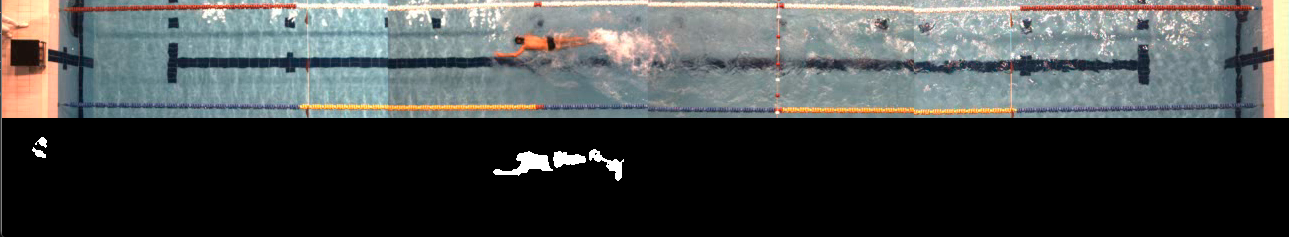
\includegraphics[width=0.9\textwidth,height=0.9\textheight,keepaspectratio]{imagenes/parte_BS/PROCESAR_SIN_BBOX_I.png} \\
          a) Fotograma A. Original y segmentación inicial. \\
          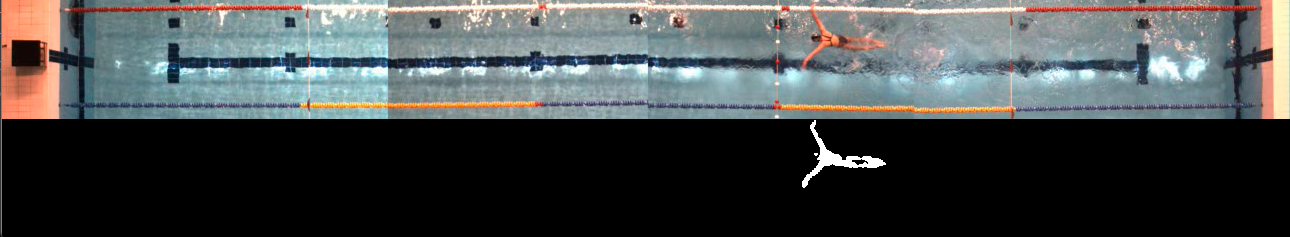
\includegraphics[width=0.9\textwidth,height=0.9\textheight,keepaspectratio]{imagenes/parte_BS/PROCESAR_SIN_BBOX_II.png} \\
          b) Fotograma B. Original y segmentación inicial. \\
     \end{tabular}
     \caption{Resultado de eliminar el fondo de la imagen utilizando GSoC sobre la banda de crominancia roja de YCbCr.}
     \label{fig:ejemplosinbbox}
\end{figure}


\section{Extracción del contorno del nadador}
\label{sec:Extraccion_contorno}
Hasta ahora hemos conseguido reconocer de manera visual al nadador, pero no hemos obtenido aún su posición en la piscina ni la zona de píxeles que le contiene. Para poder obtener una bounding box que enmarque el contorno del nadador utilizaremos la función \textit{findContours()} del paquete software OpenCV junto con un proceso de refinamiento adaptado a el modelo propuesto, y que se explica más adelante. El algoritmo implementado por dicho software se basa en \cite{contornosalgor}, y trabaja sobre imágenes binarias buscando unir aquellos píxeles con valor no nulo que estén 4-conectados u 8-conectados. Además, tiene en cuenta cuales son los píxeles externos y la jerarquía entre conexiones para poder ofrecer tolerancia a pequeños huecos que puedan producirse en el interior del objeto a delimitar.

Para nuestros experimentos, hemos utilizado las siguientes banderas: \\\textit{RETR\_EXTERNAL} y \textit{CHAIN\_APPROX\_SIMPLE}. De esta manera, sólo obtenemos las bounding box exteriores, representadas cada una de ellas por una tupla de la forma [coordenada X, coordenada Y, ancho, alto]. Este enfoque nos permite ahorrar memoria de forma significativa, ya que solo deberemos almacenar 4 valores enteros por bounding box, en lugar de las coordenadas X e Y de cada punto que conforme cada contorno, las cuales no necesitaremos.

En la figura \ref{fig:muchoscontornos} se muestran varios fotogramas, sobre los que se han dibujado rectángulos correspondientes a los contornos detectados.

\begin{figure}[h!]
    \centering
    \begin{tabular}{c}
          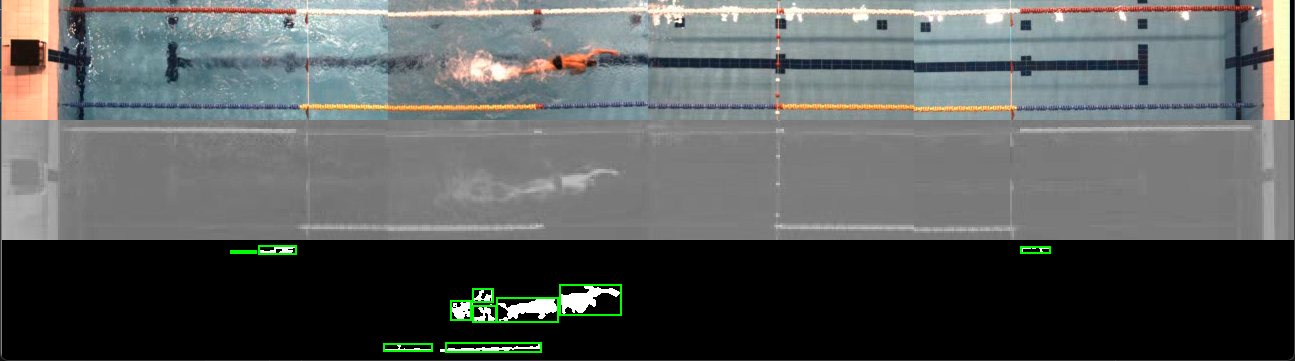
\includegraphics[width=0.9\textwidth,height=0.9\textheight,keepaspectratio]{imagenes/parte_BS/MUCHOS_CONTORNOS_I.png} \\
          a) Fotograma A y bounding boxes detectadas. \\
          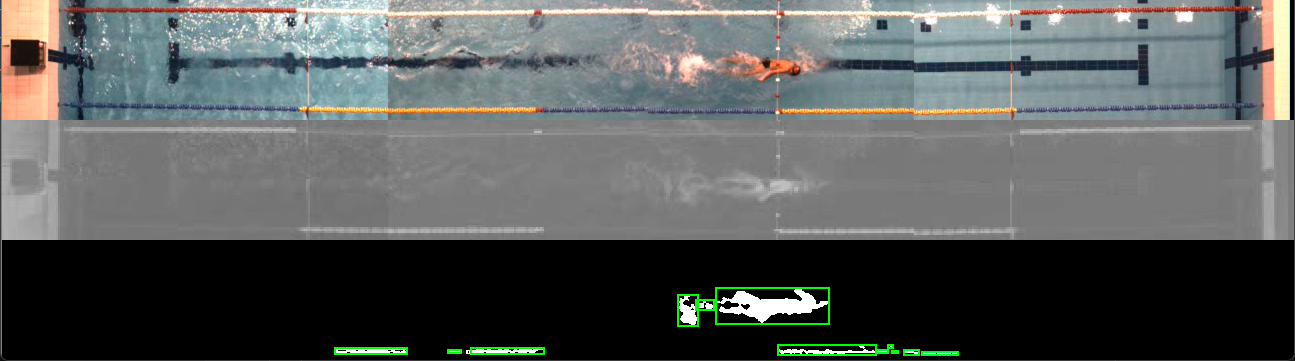
\includegraphics[width=0.9\textwidth,height=0.9\textheight,keepaspectratio]{imagenes/parte_BS/MUCHOS_CONTORNOS_II.png} \\
          b) Fotograma B y bounding boxes detectadas.\\
          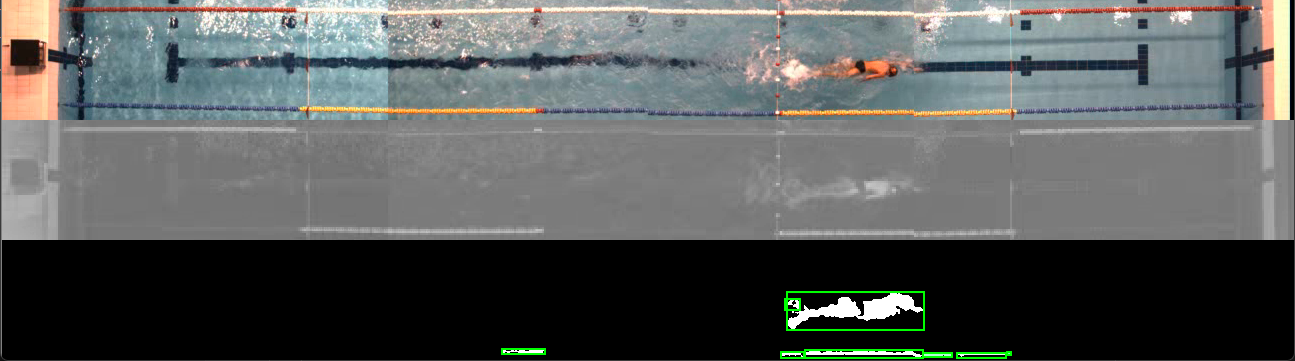
\includegraphics[width=0.9\textwidth,height=0.9\textheight,keepaspectratio]{imagenes/parte_BS/MUCHOS_CONTORNOS_III.png} \\
          c) Fotograma C y bounding boxes detectadas.\\
     \end{tabular}
     \caption{Bounding boxes detectadas sin proceso de filtrado.}
     \label{fig:muchoscontornos}
\end{figure}

Analicemos los distintos fotogramas y sus peculiaridades uno por uno. 
\begin{itemize}
    \item En el fotograma A podemos observar como se detectan múltiples bounding boxes. Particularmente, tenemos parte de las corcheras, el nadador dividido en dos - dado que el bañador no detectado genera una discontinuidad en el borde - y varios cajas correspondientes al chapoteo generado por las patadas del nadador.
    \item En el fotograma B seguimos manteniendo la detección de algunas corcheras. Sin embargo, en esta ocasión el contorno del nadador sí que es detectado como una sola entidad, bajo un único rectángulo.
    \item En el fotograma C el movimiento del agua tras el nadador es tan considerable que el algoritmo recoge al nadador y parte de dicho agua  bajo una única bounding box. Inicialmente se barajó la posibilidad de utilizar morfología matemática para intentar eliminar el efecto del chapoteo en el agua. Sin embargo, su aplicación con diversas formas y tamaños no produjo resultados satisfactorios y se descartó su uso. Ciertamente se conseguía reducir la cantidad de chapoteo reconocida como parte del nadador, pero también se desvirtuaba considerablemente el contorno del nadador, de forma que no resultaba útil para el cálculo de la frecuencia de nado.
\end{itemize}

Tras delimitar los posibles objetos, tendremos en cuenta las características de cada tipo de fotograma para diseñar un proceso de refinamiento que nos permita obtener como resultado final una única bounding box que enmarque el contorno del nadador. Los pasos que se seguirán en dicho proceso son los siguientes:

\begin{enumerate}
    \item En primer lugar discriminaremos las bounding boxes obtenidas en función de su posición en el eje X. Sólo nos interesaran aquellas que se encuentren dentro del agua de la piscina. Esta medida puede parecer innecesaria, ya que la parte del fotograma que no abarca la piscina es muy pequeña, pero no lo es. Hay ocasiones en los que el entrenador se acerca al borde del trampolín para dar instrucciones al nadador, o hay personas deambulando por esa zona. Estos sujetos no son de nuestro interés, por lo que debemos descartarlos. 
    \item A continuación, buscaremos obviar las corcheras que separan las calles de las piscinas. Dado que la posición de las corcheras no varía significativamente, ya que siempre están en los mismos lugares de la piscina y el nado de otros nadadores de calles contiguas apenas las mueven, podemos discriminarlas en función de su posición. Así pues, descartaremos los objetos cuyas coordenadas Y (superior izquierda del rectángulo) se encuentre en el 10\% superior o 10\% inferior de la calle. Además, dado que las corcheras tienen un tamaño homologado, también las discriminaremos por su altura, la cual es bastante inferior al ancho de un humano. Colateralmente, estas restricciones nos permite obviar personas que deambulen por el borde de la primera y última calle.
    \item Una vez hemos seleccionado las bounding boxes pertenecientes a la región de interés de la calle, realizaremos un filtrado en función del área. En los fotogramas de la figura \ref{fig:muchoscontornos} se puede observar que las bounding boxes que contienen al nadador son las de mayor área. Dado que el nadador puede representarse mediante dos bounding boxes, al separarse tronco de piernas, o en una única bounding box, debemos buscar valores experimentales que nos indiquen un área mínima y máxima para la cual consideramos que la bounding box puede pertenecer a un nadador. De detectarse más de dos objetos, nos quedaremos sólo con las dos bounding boxes de mayor área cuyo valor se encuentre en el rango anteriormente calculado. Esta medida nos permite obviar bounding boxes que contengan zonas de agua en movimiento debido a las patadas del nadador.
    
    \item Por último, distinguiremos en función de si tenemos una o dos bounding boxes. En caso de tener una única bounding box consideraremos que este es el nadador, mientras que en el caso de que tengamos dos bounding boxes consideraremos que podrían contener tronco y piernas del nadador e intentaremos unirlas. Tendremos en cuenta tres factores a la hora de decidir si unir las cajas o no. 
        \begin{itemize}
            \item La separación vertical entre las bounding box. La esquina superior izquierda de las bounding box que contienen tronco superior y las piernas del nadador deberían tener aproximadamente la misma posición en el eje Y, teniendo en cuenta un margen de error dado que el brazo puede estar extendido si se está realizando una brazada.
            \item La separación en el eje X entre ambas cajas. El hecho de que el nadador se detecte en dos bounding boxes separadas suele atribuirse a que el bañador no es detectado por el algoritmo de sustracción de fondos. Si la separación entre las cajas es significativamente mayor que el tamaño de un bañador consideraremos que no se deben unir.
            \item La longitud posible de la bounding box resultante de la unión. Resulta lógico descartar la unión de las bounding boxes cuando esta pueda generar resultados poco realistas. Por ejemplo, es altamente improbable que el nadador a seguir mida más de 2.3 metros. La excesiva longitud de la bounding box resultante suele producirse debido a una cantidad significativa de chapoteo detectada como parte de las piernas del nadador. Este parámetro es difícil de ajustar dada la gran variación en estatura que puede haber entre nadadores, así como la variación en el tamaño del chapoteo generado por sus patadas.
        \end{itemize}
    La unión de las bounding box sólo se realizará si los tres valores anteriormente mencionados se encuentran dentro de unos determinados rangos, calculados experimentalmente a partir de los datos que hemos podido extraer y analizar de las bounding box generadas en torno a los nadadores en varios vídeos. 
\end{enumerate}

Una vez tenemos una única bounding box, que hemos considerado que enmarca el contorno del nadador, guardaremos su posición en el eje X y su anchura. Estos datos los analizaremos en el capítulo \ref{cap:capitulo5} para poder calcular la frecuencia media de nado. Con la extracción de la bounding box ya estamos en posición de evaluar cuantitativamente las distintas combinaciones de espacio de color y algoritmo de sustracción de fondo. Los resultados experimentales se muestran a continuación en la sección \ref{sub:eleccionalgoritmo}.

\section{Evaluación experimental} \label{sub:eleccionalgoritmo}

En las secciones anteriores hemos comentado los espacios de color, algoritmos de sustracción de fondos más populares y cómo extraemos el contorno del nadador en forma de bounding box. En esta sección nos centraremos en analizar el rendimiento de nuestro método para las distintas combinaciones posibles que pueden tener lugar a partir de los espacios de color descritos en \ref{sub:elegirespaciocolor} y los algoritmos de sustracción de fondos explicados. Elegiremos aquella combinación que mejores resultados prácticos nos proporcione.

Para evaluar los resultados, usaremos los vídeos proporcionados por investigadores de la Facultad de Ciencias del Deporte de la Universidad de Granada. Sin embargo, carecemos de etiquetas sobre la posición exacta del nadador en cada fotograma. Con el objetivo de disponer de información que nos permita evaluar cuantitativamente los resultados, hemos seleccionado aleatoriamente 45 fotogramas de entre los vídeos que tenemos a nuestra disposición. Los fotogramas muestran una única calle de la piscina y se ha etiquetado manualmente el contorno del nadador mediante una bounding box.

Para realizar la comparativa emplearemos dos métricas, el índice de Jaccard y el coeficiente de Sorensen-Dice. Estos nos permitirán determinar cómo de buena es la bounding box que el algoritmo nos devuelve frente a una bounding box determinada manualmente por un humano.

\begin{itemize}
    \item El índice de Jaccard, también conocido como ``intersección sobre la unión`` (IoU), es una de las métricas más utilizadas en segmentación de imágenes debido a su sencillez y efectividad. Nos permite medir el grado de superposición de dos bounding boxes, cuanto más se solapen, mayor será el valor del índice. Su expresión matemática es la siguiente: 
    \begin{equation}
        IoU= \frac{Area\ de\ interseccion}{Area\ de\ union} = \frac{A \cap B}{A \cup B}=\frac{A\cap B}{|A|+|B|-(A \cap B)}
    \end{equation}
    \item El coeficiente de Sorensen-Dice, también conocido como F1-Score, es otra de las métricas más utilizadas, y nos permite combinar la precisión - cuantas predicciones positivas son realmente positivas - y el recall - cuántas predicciones positivas están realmente bien clasificadas - en una única métrica. Este índice trata mejor a aquellos algoritmos que consigan realizar predicciones correctas, verdaderos positivos. Su expresión matemática es la siguiente: 
    \begin{equation}
        Dice = \frac{2 \times Area\ de\ interseccion}{Suma\ de\ cardinalidades} = \frac{2 \times (A \cap B)}{|A| + |B|}
    \end{equation}
\end{itemize}

Ambos índices están positivamente correlados, es decir, si uno de ellos dice que el método A es mejor que el método B, el otro dirá lo mismo. Además, ambos índices varían en el rango [0,1]; siendo 0 una predicción totalmente incorrecta y 1 la similitud total entre las bounding boxes. 

En la figura \ref{fig:iouvisualimgs} se muestran 6 fotogramas en los que se comparan las predicciones realizadas por el algoritmo, representadas en rojo, con la segmentación realizada manualmente por un humano, en verde. En dichas imágenes se recogen situaciones a las que suele enfrentarse el algoritmo. En particular:
\begin{itemize}
    \item En los fotogramas A y B no se cumple el criterio para unir tren superior e inferior del nadador, por lo que sólo se considera la región de mayor área. Por lo general, el tren superior ocupa un mayor área que el tren inferior, especialmente si los brazos se encuentran estirados o se está realizando una brazada.
    \item En los fotogramas C y D sí que se detecta al nadador completo, pero también se considera como parte del nadador una buena parte del chapoteo que genera su avance por el agua. Como veremos posteriormente, esto disminuirá la calidad de la segmentación realizada.
    \item En los fotogramas E y F se consigue detectar al nadador sin incluir casi chapoteo alguno. Este es el caso que desearíamos que siempre se produjera.
\end{itemize}  

Con el objetivo de ilustrar el comportamiento de las métricas ante distintas situaciones, en la tabla \ref{tab:iouvisualtab} se recogen los valores de los índices de Jaccard y Sorensen-Dice para cada fotograma de la figura \ref{fig:iouvisualimgs}. Si se comparan los valores numéricos con los resultados visuales, se pueden extraer importantes conclusiones:
\begin{itemize}
    \item Las predicciones en las que sólo se detecte correctamente a medio nadador tienen valores de los coeficientes de Jaccard y Sorensen-Dice bajos. Sus valores suelen oscilar en el rango [0.2; 0.45]. 
    \item En el caso de detectar como parte del nadador chapoteo del agua, el valor de los índices se mueve en un rango relativamente amplio. En los casos extremo en los que se detecta todo el chapoteo como parte del nadador, como en el fotograma C, el índice de Jaccard tiene un valor en el rango [0.3; 0.37] aproximadamente. Si se detecta poco chapoteo el valor del índice de Jaccard suele encontrarse en el rango [0.55; 0.65]. Podríamos considerar como buenas predicciones, por tanto, aquellas que superen un valor IoU de 0.55.
    \item En el caso de detecciones muy buenas, como en el fotograma E, o prácticamente perfectas, como en fotograma F, el índice de Jaccard tiene un valor en el rango [0.8; 0.9], mientras que el índice de Sorensen-Dice se mueve en el rango [0.88; 0.95].
\end{itemize}
 
\begin{figure}[h!]
    \centering
    \begin{tabular}{cc}
          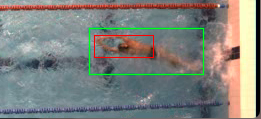
\includegraphics[width=0.43\textwidth,height=0.43\textheight,keepaspectratio]{imagenes/parte_BS/iou_visual/mala_1099.png} &
          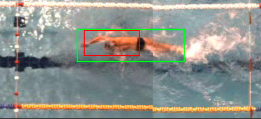
\includegraphics[width=0.43\textwidth,height=0.43\textheight,keepaspectratio]{imagenes/parte_BS/iou_visual/medio_cuerpo_1259.png}
          \\ Fotograma A   & Fotograma B \\
          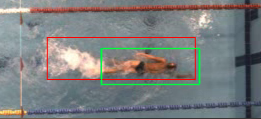
\includegraphics[width=0.43\textwidth,height=0.43\textheight,keepaspectratio]{imagenes/parte_BS/iou_visual/muchisima_agua_1014.png} &
          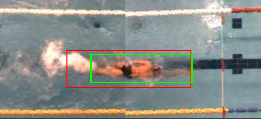
\includegraphics[width=0.43\textwidth,height=0.43\textheight,keepaspectratio]{imagenes/parte_BS/iou_visual/mucha_agua_897.png}
          \\ Fotograma C & Fotograma D \\
          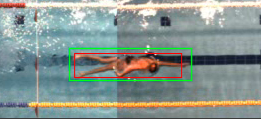
\includegraphics[width=0.43\textwidth,height=0.43\textheight,keepaspectratio]{imagenes/parte_BS/iou_visual/excelente_611.png} &
          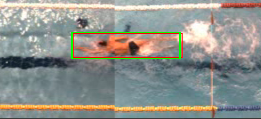
\includegraphics[width=0.43\textwidth,height=0.43\textheight,keepaspectratio]{imagenes/parte_BS/iou_visual/excelentisimo_1241.png}
          \\Fotograma E & Fotograma F
     \end{tabular}
     \caption{Predicción automática (en rojo) frente a segmentación manual (en verde) para diferentes fotogramas}
     \label{fig:iouvisualimgs}
\end{figure}

\begin{table}[h!]
    \centering
    \begin{tabular}{| c | c | c | } \hline
        Fotograma & IoU & Sorensen-Dice \\ \hline
        A & 0.23627 & 0.38223  \\
        B & 0.40158 & 0.57304 \\   
        C & 0.35484 & 0.52381 \\ 
        D & 0.60322 & 0.75251 \\ 
        E & 0.82480 & 0.90399 \\ 
        F & 0.87036 & 0.93069 \\ \hline
    \end{tabular}
    \caption{Métricas para predicciones frente a segmentación manual}
    \label{tab:iouvisualtab}
\end{table}


\begin{table}
    \centering
    \begin{tabular}{| c | c | c | c | c|}\hline
        %\multirow{number rows}{width}{text} &  \\
        Banda & Algoritmo & IoU & Dice & T.ejecución (ms) \\ \hline
        \multirow{3}{*}{S de HSV} & KNN  & 0.47256 & 0.56733 & 5.530 \\
        &MOG2 & 0.49366 & 0.59887 & 5.457 \\
        &GSoC & 0.48128 & 0.57142 & 11.778 \\ \hline
        \multirow{3}{*}{Cb de YCbCr} & KNN  & 0.14175 & 0.22651 & \textbf{3.918} \\
        &MOG2 & 0.39959 & 0.53033 & 4.099 \\
        &GSoC & 0.47209 & 0.61864 & 10.939 \\ \hline
        \multirow{3}{*}{Cr de YCbCr} & KNN  & 0.39881 & 0.55140 & 4.423 \\
        &MOG2 & 0.56134 & 0.68497 & 4.413 \\
        &GSoC & \textbf{0.64126} & \textbf{0.76864} & 11.051 \\ \hline
    \end{tabular}
    \caption{Comparativa de rendimiento}
    \label{tab:rendimientofondoscap3}
\end{table}

En las tablas de la figura \ref{tab:rendimientofondoscap3} se muestran los resultados experimentales obtenidos en media para todo el dataset de evaluación. Adicionalmente, se proporciona el tiempo medio en milisegundos que ha demorado la ejecución para cada fotograma de un vídeo de 2025 fotogramas de longitud. 

Analicemos los resultados de las tablas anteriores para elegir una combinación de espacio de color y algoritmo de sustracción de fondos a utilizar.
\begin{itemize}
    \item Para el caso del canal de saturación de HSV podemos concluir que la influencia del algoritmo de sustracción es muy pequeña. Los algoritmos K-NN y GSoC nos devuelven valores prácticamente iguales para las métricas consideradas, siendo el algoritmo MOG2 el que ofrece resultados ligeramente mejores, con un valor IoU 0.015 mayor. Si tuviéramos que trabajar en esta banda la elección más recomendable, bajo nuestra opinión, sería el algoritmo MOG2. Esto es debido a que la diferencia de rendimiento respecto de los demás algoritmos no es demasiado significativa, y el tiempo de ejecución es similar al de KNN. Las métricas nos indican que el uso de esta banda nos devolvería predicciones que podríamos considerar acertadas, pero no excelentes.
    \item En la banda de crominancia azul de YCbCr sí que notamos diferencia al utilizar distintos algoritmos. El algoritmo K-NN ofrece resultados pésimos, al proporcionar un valor del índice de Jaccard significativamente menor a 0.3. MOG2 y GSoC ofrecen predicciones algo más certeras, siendo GSoC el que mejor se comporta. En virtud de los valores experimentales podemos concluir que el uso de esta banda no ofrece mejora alguna respecto de la banda de saturación de HSV, por lo que la descartamos como posible elección.
    \item Los mejores resultados medios los obtenemos haciendo uso del canal de crominancia roja de YCbCr. Para este canal, el algoritmo con menor rendimiento (K-NN) ya proporciona resultados que podríamos considerar aceptables, al tener un valor del índice de Jaccard de 0.4. Sin embargo, podemos observar que el algoritmo GSoC obtiene un resultado medio bastante mejor, con un valor de los índices IoU y Sorensen-Dice de 0.64 y 0.769, respectivamente. Si comparamos estos valores con los mostrados en la tabla \ref{tab:iouvisualtab}, correspondientes a los fotogramas de la figura \ref{fig:iouvisualimgs}, podemos concluir que las predicciones son ciertamente buenas, y como veremos posteriormente en el capítulo \ref{cap:capitulo5}, suficientes para realizar la estimación de las brazadas por minuto del nadador. A pesar de que GSoC requiere algo más del doble de tiempo de cómputo que otros algoritmos, podríamos satisfacer condiciones de tiempo real si fuese necesario. Si tenemos en cuenta que los vídeos proporcionados por los investigadores tienen una tasa de 41.66 fotogramas por segundo necesitaríamos procesar y mostrar un fotograma cada 24 milisegundos para mantener la fluidez del vídeo. Dado que ambos métodos ofrecen un tiempo de ejecución considerablemente menor a los mencionados 24 milisegundos podemos elegir cualquiera de ellos. Por tanto, elegiremos la banda de crominancia roja de YCbCr y el algoritmo GSoC para realizar la detección del nadador al ser los que mejores resultados proporcionan. 
\end{itemize}

Por último, se debe tener en cuenta que se requieren unos doscientos fotogramas, aproximadamente, para entrenar el modelo del sustractor de fondos GSoC, de manera que se produzca la eliminación del fondo con el nivel de rendimiento esperado. En el dominio de nuestro problema, 200 fotogramas equivalen a unos 4.5 segundos. Si tenemos en cuenta el tiempo que toma iniciar la grabación y avisar al entrenador de que puede indicar la salida al nadador, la preparación del propio nadador, y el inicio de la prueba, el entrenamiento del modelo se realiza a tiempo, por lo que no encontramos problemas prácticos. Cuando el nadador se lanza a la piscina el modelo ya es capaz de categorizar la inmensa mayoría del agua como elemento estático y realizar una correcta eliminación del fondo.

Tras analizar el método que utilizaremos para detectar al nadador a lo largo de la piscina siguiendo técnicas clásicas del procesamiento de imágenes, en el siguiente capítulo se comentará un método para realizar la detección haciendo uso de técnicas de aprendizaje profundo y redes neuronales.
	\chapter{Detección de nadadores mediante técnicas de aprendizaje profundo} \label{cap:capitulo4}

Los últimos avances en detección de nadadores hacen uso de técnicas de aprendizaje profundo. En este apartado haremos uso de la popular red de detección de objetos YOLO, siguiendo a los trabajos \cite{comparisoncnnscoches} \cite{comparativaseniales} \cite{rcnnvsyolodivers}, para establecer una comparativa con la aproximación presentada en el capitulo \ref{cap:capitulo3}.

Al principio de este capítulo se realizará una pequeña introducción a las redes neuronales convolucionales. En secciones posteriores se ahondará en el modelo YOLO para la detección de objetos, el entrenamiento que se ha realizado para que la red neuronal sea capaz de reconocer a los nadadores y el análisis de los resultados experimentales obtenidos.


\section{Introducción a las redes neuronales}


Las redes neuronales artificiales (ANN) son sistemas de procesamiento de información que se inspiran en gran medida en el funcionamiento de sistemas nerviosos complejos, como el cerebro humano \cite{rnatheoryi}. Las ANN están compuestas por un número muy elevado de nodos computacionales interconectados, que reciben el nombre de neuronas. Estas neuronas artificiales trabajan de forma distribuida para aprender a partir de una serie de estímulos de entrada, de manera que sean capaces de ofrecer una respuesta a esos estímulos y otros similares. 

Las redes neuronales convolucionales (CNN) son un tipo de ANN cuya estructura se basa en el funcionamiento de las neuronas de la corteza visual primaria (V1) de un cerebro biológico, como podría ser el de un gato o el de un humano \cite{reviewcnn}. 

Estas redes neuronales se pueden entender como cajas negras que siguen una metodología de aprendizaje supervisado ``data-driven'', basada en datos. A partir de una serie de datos de entrenamiento, en nuestro caso imágenes y etiquetas sobre dichas imágenes, la red neuronal optimiza multitud de parámetros, en ocasiones millones \cite{rnatheoryi}. El objetivo final de este proceso es hacer que la red neuronal adquiera la habilidad de reconocer, distinguir y localizar objetos en nuevas imágenes que se puedan proporcionar como entrada, distintas a las usadas durante el entrenamiento.

Dado que el objetivo de este trabajo no es el análisis pormenorizado de la arquitectura de las redes neuronales convolucionales, a continuación sólo se proporcionará una descripción general de los elementos que suelen constituir las CNN. El lector interesado en ellas puede consultar \cite{cnnindetail}.

\begin{itemize}
    \item Las capas convolucionales son los elementos más importantes de una CNN. Estas capas aplican operaciones de convolución con distintos filtros sobre la imagen completa o partes de esta. Este procedimiento permite extraer características significativas que se utilizarán para reconocer y distinguir objetos.
    \item La función de activación es una función matemática que calcula un valor a partir de la suma ponderada de los datos que percibió la neurona. Se suele aplicar tras cada capa convolucional para decidir si la neurona debe activarse o no. En el caso de las CNN se suelen emplear funciones no lineales, pero podrían ser lineales.
    \item En las capas ``pooling'' se tiene como objetivo generalizar las características extraídas por las capas convolucionales y ayudar a la red a reconocer las características independientemente de su ubicación en la imagen. Se utilizan para disminuir y aumentar el tamaño de las capas, normalmente generando una estructura de cuello de botella que obliga a sintetizar la información.
    \item En las capas totalmente conectadas, como su propio nombre indica, cada neurona está conectada con cada una del resto de neuronas de la capa anterior. Al final de la CNN suele haber una o varias de estas capas, de forma que la salida de la última es el resultado devuelto por la CNN.
    \item Por último, se fija una función de perdida o función objetivo. Esta función evaluará el nivel de error que existe entre las predicciones realizadas por la red neuronal y los valores reales proporcionados como etiquetas. El resultado de esta función, permitirá optimizar los parámetros de la red para obtener las predicciones deseadas. 
\end{itemize}

\section{YOLO para detección de objetos}

``You Only Look Once'', abreviado como YOLO, es una arquitectura de detección de objetos creada por Joseph Redmond en 2016, y cuya especificación se detalla en el artículo \cite{yolooriginalpaper}. La arquitectura YOLO emplea CNNs para detectar objetos, y como su nombre puede sugerir, sólo se requiere de una única propagación de la imagen de entrada a lo largo de la red neuronal para realizar detecciones de múltiples objetos.

El autor continuó desarrollando la arquitectura y lanzó una segunda versión en 2017 \cite{yolov2originalpaper}, y una tercera versión en 2018 \cite{yolov3originalpaper}. En febrero de 2020, Joseph Redmond publicaba en su cuenta de Twitter (@pjreddie) que abandonaba su investigación en visión por computador debido a preocupaciones éticas de cómo la tecnología que había desarrollado se estaba usando. Sin embargo, su trabajo fue continuado por numerosos investigadores, quienes propusieron nuevas mejoras y versiones. YOLOv4, propuesta por Alexey Bochkovski en abril de 2020 \cite{yolov4originalpaper}, puede ser considerada la versión más popular actualmente, y fue la reconocida por el propio Joseph Redmond como ``la versión canónica''. 

Las cuatro primeras versiones fueron desarrolladas haciendo uso de Darknet, una librería de código libre para implementar redes neuronales escrita en \textit{C} y \textit{CUDA}. En la actualidad comienzan a surgir versiones, como YOLOv5 \cite{yolov5pseudopaper}, cuya implementación se realiza haciendo uso de otros frameworks, como PyTorch o Tensorflow.

Aunque no profundizaremos en ello en este trabajo, es interesante mencionar que YOLO se ha comparado en la literatura con otras aproximaciones a la detección de objetos, especialmente con las arquitecturas de la familia R-CNN (Region-based convolutional neuronal network) y SSD (Single Shot Detector). La familia R-CNN analiza la imagen en dos propagaciones a traves de la red: una de extracción de regiones de interés y otra de propagación de cada región de interés por la CNN. Por otro lado, SSD es un algoritmo de detección de una única fase. Al igual que YOLO, tan solo necesita una única propagación. 
En los trabajos \cite{comparisoncnnscoches} y \cite{comparativaseniales} se puede consultar una de estas comparativas entre arquitecturas. Sus resultados muestran que YOLOv3, y especialmente YOLOv4, son las aproximaciones a la detección de objetos que presentan menores tiempos de procesamiento y mayor precisión media en sus detecciones. En \cite{comparativaseniales} también se concluye que YOLOv4 requiere un menor tiempo de entrenamiento. Además, se ha utilizado con anterioridad~\cite{rcnnvsyolodivers} en entornos acuáticos. En virtud de los datos proporcionados por estos estudios, se decide utilizar YOLOv4 para realizar la detección de los nadadores en este trabajo

A continuación introducimos, a alto nivel, los conceptos más relevantes para comprender la arquitectura de YOLOv4.  En términos generales, la arquitectura completa de un detector de objetos suele estar compuesta por dos partes, en la literatura se conocen como la ``columna vertebral'' (``backbone'') y la ``cabeza'' (``head''). La ``columna vertebral'' es un extractor de características, pre-entrenado para realizar tareas de clasificación, mientras que la cabeza es la encargada de predecir las coordenadas de las bounding box y el tipo de objeto. 

En el caso de YOLO, la ``columna vertebral'' es alguna variante de Darknet (Darknet-19 para YOLOv2, Darknet-53 para YOLOv3). En las tres primeras versiones de YOLO la arquitectura sólo consta de columna vertebral y cabeza, pero a partir de YOLOv4 se introduce el cuello (``neck''), un elemento adicional que conecta los otros dos, y permite extraer características a distintos niveles del ``backbone''.

En la figura \ref{fig:yoloconvolutionlayers} se puede apreciar la arquitectura de la ``columna vertebral'' de la red neuronal convolucional para la primera versión de YOLO. Se puede apreciar como la sucesión de capas convolucionales, de pooling y totalmente conectadas extraen de la imagen un conjunto de características de menor dimensión que la imagen.

\begin{figure}[]
    \centering
    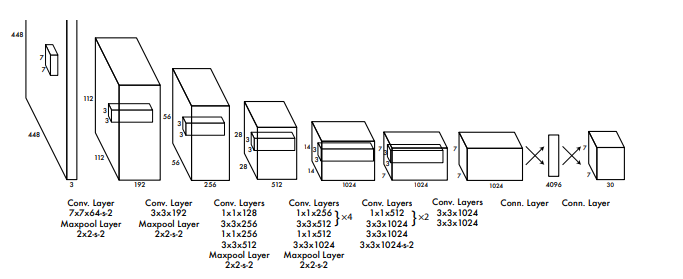
\includegraphics[width=0.9\textwidth,height=0.9\textheight,keepaspectratio]{imagenes/parte_IA/YOLOv1-architecture.png}    
    \caption{Arquitectura de la ``columna vertebral'' de YOLOv1.}
    \label{fig:yoloconvolutionlayers}
\end{figure}

\begin{figure}[]
    \centering
    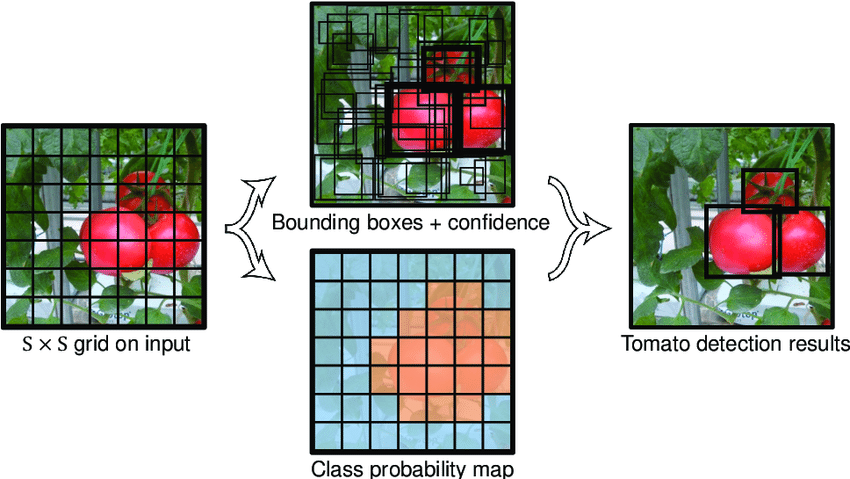
\includegraphics[width=0.78\textwidth,height=0.78\textheight,keepaspectratio]{imagenes/parte_IA/YOLO-simplify-steps.png}    
    \caption{Esquema del funcionamiento básico de YOLO.}
    \label{fig:yolosimplify}
\end{figure}

El funcionamiento de YOLO se muestra de forma simplificada en la figura \ref{fig:yolosimplify}. La cuarta versión \cite{yolov4originalpaper} se describe de forma general a continuación.

\begin{itemize}
    \item Primero se divide la imagen de entrada en cuadrículas de tamaño PxP píxeles. Cada cuadrícula será la responsable de detectar y localizar los objetos cuyo centro se encuentren en ella. El número de objetos que se pueden detectar por celdas varía en función de la versión utilizada; en la primera versión sólo se podía detectar un único objeto por celda, pero este valor ha ido aumentando en las versiones sucesivas.
    \item Tras dividir la imagen, esta se pasa por la red neuronal convolucional. Como resultado, en cada una de las celdas se predice un número B de objetos, estando representado cada objeto por un vector de 5+C elementos, donde C es el número de clases de objetos que podemos distinguir. Dicho vector tendrá la forma \\ $\rvect{P_c,B_x, B_y,B_w,B_h,C_1,C_2,...}$, donde:
    \begin{itemize}
        \item $P_c$ hace referencia a la confianza con la que se realiza la predicción de un objeto. Equivale al valor del índice de Jaccard entre la bounding box predicha y la supuesta bounding box real. Un valor de 0 indica que no se ha detectado ningún objeto, mientras que un valor 1 indica que se está completamente seguro de que hay un objeto contenido exactamente por la bounding box predicha.
        \item $B_x, B_y, B_w, B_h$ indican la posición X e Y del centro de la bounding box, así como el ancho y el alto de la misma. Los valores no se indican en unidades absolutas, como píxeles, si no que son proporcionales al ancho y alto de la celda.
        \item $C_0, C_1, ...$ indican si el objeto detectado corresponde a la clase de objeto con etiqueta 0, etiqueta 1, etc. Sólo uno de estos valores será 1, siendo el resto 0, ya que un objeto sólo puede pertenecer a una única clase.
    \end{itemize}
    Téngase en cuenta que si $P_c = 0$, el resto de valores del vector pueden ser ignorados, al no haberse detectado objeto alguno.
    \item Los cálculos anteriores generan multitud de predicciones duplicadas. Esto se debe a que varias celdas pueden haber detectado el mismo objeto, pero con bounding boxes diferentes. Por tanto, se debe utilizar algún mecanismo que nos permita seleccionar la mejor bounding box para cada objeto, descartando el resto. En particular, YOLO utiliza la técnica de la ``supresión de no máximos''.  
    \item La técnica de la ``supresión de los no máximos'' selecciona la bounding box con el valor $P_c$ (confianza en la predicción) más alto para cada etiqueta de clase y elimina las bounding boxes con la misma etiqueta de clase que se superpongan mucho con la caja seleccionada inicialmente. Normalmente se considera que las cajas se superponen mucho si se tiene un valor del índice de Jaccard igual o superior a 0.5. Este procedimiento se repite hasta que no se pueda eliminar ninguna bounding box más. En la figura \ref{fig:yolonmsexample} se puede apreciar la aplicación de este procedimiento, de manera que se obtiene como resultado una única bounding box para cada objeto, en este caso, de clases distintas. 
    \item Como resultado del proceso anterior, se retorna un vector de 6 elementos por cada objeto detectado. Los 5 primeros elementos coinciden con los del vector mostrado en puntos anteriores, siendo el sexto elemento el número de la etiqueta de clase del objeto detectado. Por tanto, los vectores resultantes tienen la forma $\rvect{P_c,B_x, B_y,B_w,B_h,C_N}$ 
\end{itemize}

\begin{figure}[]
    \centering
    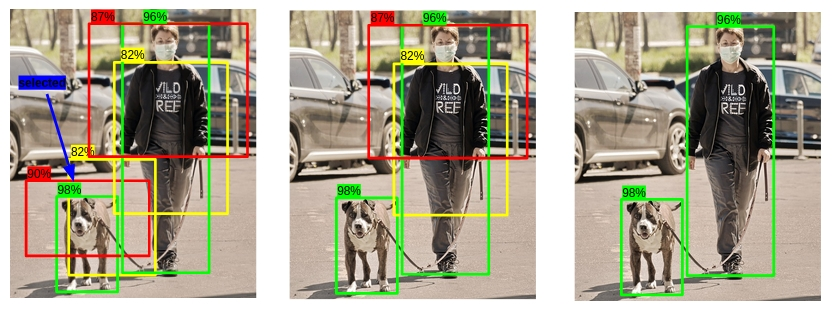
\includegraphics[width=0.9\textwidth,height=0.9\textheight,keepaspectratio]{imagenes/parte_IA/nms_yolo.jpg}    
    \caption{Aplicación de la supresión de no máximos.}
    \label{fig:yolonmsexample}
\end{figure}

Tras conocer el modus-operandi del detector de objetos YOLO, en la siguiente sección se explicarán los detalles del entrenamiento que se ha realizado para que este sea capaz de reconocer nadadores.

\section{Entrenamiento del modelo YOLOv4 para la detección de nadadores} 

En esta sección se detalla el proceso que se ha llevado a cabo para entrenar el modelo YOLOv4 de manera que sea capaz de detectar a los nadadores.

La primera decisión que se abordó fue si entrenar la red neuronal desde cero o utilizar los resultados de algún entrenamiento disponible en Internet y realizar un ajuste de manera que la red se especializara en la detección de nadadores.

Se optó por la segunda opción. Utilizamos un fichero de pesos resultado de haber entrenado la red en el conjunto de datos de prueba COCO (Common Objects in Context) \cite{cocodataset}. Esta base de datos está compuesta por unas 328.000 imágenes, entre las que se pueden reconocer 2.5 millones de objetos de 80 categorías distintas. Sin embargo, lo que hace esta base de datos especialmente adecuada para nuestra tarea es que tiene etiquetadas unas 250.000 personas. Así, la red neuronal ya posee de partida la capacidad de reconocer personas en multitud de situaciones. 

Sin embargo, este entrenamiento previo no es suficiente para conseguir detectar nadadores. Esto se debe principalmente a dos factores:
\begin{itemize}
    \item Las personas con las que ha sido entrenada la red siempre se encuentran en posición vertical, a diferencia de los nadadores, que se mueven a lo largo del eje horizontal de la piscina.
    \item En el conjunto de entrenamiento hay personas sin camiseta, con pantalones cortos (e incluso pañales), de espaldas, etc. Sin embargo, no hay apenas imágenes en las que haya personas en un ambiente en el que el agua es la componente principal, y además existan reflejos y cambios notables en la iluminación.
\end{itemize}
El primero de los problemas tiene fácil solución, rotar la imagen antes de hacer que la red neuronal la procese, de manera que el nadador estaría en vertical. Por desgracia, el segundo problema hace que la red no sea capaz de detectar a los nadadores en la gran mayoría de ocasiones.

Para solventar este inconveniente se hará uso de la técnica conocida como ``fine tuning''. Esta técnica consiste en, dada una red pre-entrenada en una base de datos distinta a la que se va a utilizar, realizar un pequeño segundo entrenamiento para mover el óptimo de la red hacia el óptimo de nuestro problema \cite{cnnindetail}. Esto nos permite enseñarle a la red a realizar una segunda tarea, en este caso el reconocimiento de nadadores, similar a la tarea en la que fue inicialmente entrenada, el reconocimiento de personas (entre otros objetos). Este enfoque nos permite reducir el tiempo de entrenamiento considerablemente, así como el número de imágenes de muestras necesarias para conseguir una correcta generalización y aprendizaje. 

El conjunto de imágenes utilizadas para el entrenamiento ha sido proporcionado por investigadores de la Facultad de Ciencias del Deporte de la UGR. El dataset consta de 1970 imágenes de resolución 120x120 píxeles en las que un nadador en posición vertical ocupa la mayor parte de cada imagen. Para cada una de estas imágenes se tiene un fichero de texto plano en el que se encuentra la etiqueta correspondiente en formato YOLO (numero de clase, coordenadas X e Y del centro de la bounding box, ancho y alto de la bounding box). En el conjunto de imágenes se tienen nadadores practicando diferentes estilos, así como momentos en los que los brazos del nadador están acoplados al cuerpo y momentos en los que se está realizando la voltereta con la que cambiar el sentido de nado al final de un split. 

Además, durante el entrenamiento se aplican técnicas de aumento de datos, entre las que se encuentran variaciones de la saturación, exposición y color de la imagen, redimensiones y recortes de la imagen, añadido de ruido gaussiano, etcétera. 

El software necesario para ejecutar YOLOv4 puede descargarse desde el repositorio oficial del autor \cite{darknetgithub}, Alexey Bochkovski. Para realizar la configuración seguiremos el manual que se proporciona y aplicaremos algunos consejos que se proporcionan en la sección wiki.

Los pasos seguidos para realizar el entrenamiento del modelo han sido los siguientes:

\begin{enumerate}
    \item Modificar los ficheros de configuración que serán utilizados para el entrenamiento. Primero, se crea una copia del fichero \textit{yolov4-custom.cfg}, ubicada en el directorio \textit{cfg}. Para este fichero, que se usará durante el entrenamiento, se realizan los siguientes cambios:
    
    \begin{itemize}
        \item \textit{Batch=32} y \textit{subdivisions=32}. El primer parámetro indica el número de imágenes que serán procesadas en un lote, mientras que el segundo se utiliza para calcular el número de mini lotes que serán procesados en paralelo por la GPU. Este valor será igual al resultado de dividir \textit{batch} y \textit{subdivisions}. Los valores de estos parámetros deben ser ajustados en función de la memoria de la que disponga la GPU. El autor recomienda mantener \textit{batch=64} siempre que se utilice una única tarjeta gráfica y modificar sólo el valor \textit{subdivisions}. Con la tarjeta gráfica de la que se disponía, NVIDIA GeForce GTX 1080, sólo se podían emplear combinaciones que tuvieran ambos valores iguales, en caso contrario se generaba un error por falta de memoria en la GPU. Se probó con valores iguales a 32 y 64, obteniendo resultados ligeramente mejores con 32.
        \item \textit{Width=416} y \textit{height=416}. Estos son el ancho y alto a los que se redimensionarán las imágenes al entrar a la red neuronal. Cuanto mayor sea este valor, mejor será el aprendizaje de la red. El autor recomienda cambiarlo a 608x608 o valores múltiplos de 32 superiores de ser posible. Sin embargo, cambiar el tamaño a 608x608 multiplicaba por cuatro el tiempo de entrenamiento, de manera que este podía llegar a alcanzar las 60 horas según las estimaciones realizadas por el propio software. Se tuvo que descartar al no ser asumible.
        \item \textit{Max\_batches=6000}. Este valor indica el número de iteraciones que tendrá el entrenamiento. Se recomienda asignar el resultado de multiplicar el número de tipos de objetos distintos que queramos detectar por 2000. En cualquier caso, el valor no debe ser inferior al número de imágenes de entrenamiento ni a 6000. Dado que solo teníamos una clase de objetos y 1970 imágenes, se asigno el valor 6000.
        \item \textit{Steps=4800,5400}. Este parámetro debe tener los valores correspondientes al 80 y 90\% del valor \textit{Max\_batches}.
        \item Para la última capa convolucional antes de cada una de las tres capas marcada como [yolo], deberemos cambiar el número de filtros por un valor tal que $filters=(classes+5)*3$. Por lo tanto, dado que sólo buscamos reconocer un tipo de objeto, se debe asignar \textit{filters=18} en las líneas 963, 1051 y 1139. Las capas marcadas como [yolo] son aquellas donde se realiza la detección de objetos. Cada una de ellas lo hace a diferente escala, de manera que se pueden detectar objetos de distinto tamaño.
        \item En las capas marcadas como [yolo] deberemos cambiar el parámetro \textit{classes} para que sea igual al número de tipos de objetos distintos que queramos distinguir. Por lo tanto, se debe asignar \textit{classes=1} en las líneas 970, 1058 y 1146. Nótese que aunque hay que reconocer una sola clase, el problema no es trivial, puesto que hay que ajustar las coordenadas de la bounding box que enmarcan al nadador. 
    \end{itemize} 
    
    A la hora de realizar la detección, deberemos crear un objeto de la clase \textit{dnn\_DetectionModel} de \textit{OpenCV}. Este constructor necesitará el fichero de configuración utilizado a la hora de entrenar y el fichero de pesos obtenido como resultado. En el código \textit{Python} se deberá establecer el tamaño al que se redimensionarán las imágenes antes de entrar a la red. Discutiremos la influencia de este parámetro en la sección \ref{evaluacionexpyolo}.
    
    \item Cargamos el conjunto de imágenes de entrenamiento, así como los ficheros de texto con las etiquetas, en el directorio \textit{data/obj}.
    
    \item Se deben crear dos ficheros de texto, \textit{data/train.txt} y \textit{data/valid.txt}, que contendrán las rutas a las imágenes que se utilizarán para el conjunto de entrenamiento y el conjunto de validación, respectivamente. Para realizar esta tarea se ha preparado un pequeño script que asigna el 85\% de las imágenes al conjunto de entrenamiento y el 15\% restante al conjunto de validación.
    
    \item Se debe crear el fichero \textit{data/obj.names}. Este contendrá los nombres de cada uno de los tipos de objetos a reconocer, uno por fila. Para este problema, sólo contendrá el valor ``person''. Debe tenerse cuidado y listar los nombres con el mismo orden que se utilizó al etiquetar los datos.
    
    \item Se tiene que crear el fichero \textit{data/obj.data}. Este contendrá el número de clases que queremos detectar, las rutas a los ficheros \textit{data/train.txt}, \textit{data/test.txt} y \textit{data/obj.names}, y la ruta al directorio donde guardaremos los ficheros generados como resultado del entrenamiento.
    
    \item También deberemos modificar las primeras líneas del fichero \textit{Makefile} para permitir el uso de la GPU, \textit{OpenCV} y \textit{CUDNN} (una librería para redes neuronales desarrollada por NVIDIA). En caso de disponer de una tarjeta gráfica con los llamados ``tensor cores'', habilitar el parámetro \textit{CUDNN\_HALF} permite reducir el tiempo de entrenamiento y detección considerablemente, en función de la resolución utilizada entre 2 y 4.5 veces \cite{darknetgithub}. Para habilitar estas opciones simplemente cambiaremos el valor 0 por el valor 1. Una vez se hayan realizado las modificaciones, se ejecutará el comando \textit{make} para generar el fichero ejecutable.
    
    \item Se debe descargar el fichero con los pesos resultantes de entrenar la red con el dataset COCO. Este fichero tiene como nombre \textit{yolov4.conv.137} y se puede encontrar en las publicaciones del repositorio \cite{darknetgithub}.
    
    \item Una vez se ha preparado todo lo necesario, deberemos ejecutar \textit{./darknet detector train data/obj.data cfg/yolov4-custom.cfg ../yolov4.conv.137 -dont\_show -map} para iniciar el entrenamiento de la red neuronal. 
\end{enumerate}

El primer entrenamiento del modelo que realizamos duró unas 7 horas y media aproximadamente. El software, al finalizar, mostraba por pantalla que se había alcanzado una precisión y recall de 1, es decir, todos los casos positivos habían sido clasificados correctamente. Esto es lógico dado que todas las detecciones realizadas corresponderían a la única clase que habíamos especificado. El valor medio del índice de Jaccard para predicciones realizadas con una confianza mínima del 25\% (mAP@0.25) era de 0.89, por lo que se había alcanzado un nivel de acierto en las predicciones muy alto. Los resultados obtenidos eran ciertamente prometedores.

Con este primer modelo, se realizó el primer intento de detección de nadadores para cada fotograma de un video. Sin embargo, a pesar de las métricas tan prometedoras obtenidas durante el entrenamiento, el modelo no era capaz de ubicar al nadador en ningún momento.

Analizando los resultados, el motivo es bastante directo. La red redimensiona las imágenes a su entrada, por tanto, cuando las imágenes de entrenamiento, de resolución 120x120 píxeles se redimensionan a un tamaño de 416x416 píxeles se mantiene la relación de aspecto, siguen siendo cuadradas, y el nadador no sufre ningún cambio. Sin embargo, los fotogramas de vídeo donde necesitamos detectar al nadador contienen una calle completa de la piscina, y tienen una resolución 120x1292 (relación 10.77:1). Redimensionar a un tamaño cuadrado, provoca que se deforme notablemente la figura del nadador, la cual no coincidirá con los ejemplos en los que la red neuronal se entrenó y hará que no se detecte nunca a dicho nadador. Esto se puede observar muy claramente en la figura \ref{fig:ejemplomalredimension}.

\begin{figure}
    \centering
    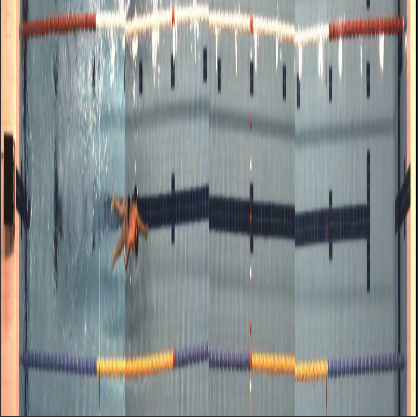
\includegraphics[width=0.5\textwidth,height=0.5\textheight,keepaspectratio]{imagenes/parte_IA/416x416_YOLO_resize.png}
    \caption{Redimensión de una calle de la piscina a tamaño cuadrado.}
    \label{fig:ejemplomalredimension}
\end{figure}

Para conseguir detectar a los nadadores se modificó el tamaño al que la red neuronal redimensiona los fotogramas del vídeo antes de procesarlos, con el objetivo de evitar que se modifique en exceso la apariencia del nadador. De esta manera, se consiguió que la red detectara a los nadadores a lo largo de la calle. Se han utilizado distintos tamaños de entrada, que se discuten en detalle en la sección \ref{evaluacionexpyolo}.

El siguiente problema apareció cuando los nadadores realizaban el giro y empezaban a nadar en sentido contrario. A partir de este momento, el nadador dejaba de ser detectado. La razón es que todos los datos de entrenamiento corresponden a nadadores en un único sentido. Esto afecta a la capacidad de detección de la red, que es incapaz de detectar a los nadadores que nadan en sentido contrario. 

Para solucionar este problema, se incluyó el volteo vertical entre las técnicas de aumento de datos, generando de esta forma las imágenes necesarias para detectar nadadores en el sentido contrario. 

Con esta nueva configuración, se realizó un nuevo entrenamiento de la red neuronal, el cual duró unas 16 horas aproximadamente. Tras este segundo entrenamiento, la red neuronal sí fue capaz de detectar a los nadadores a lo largo de todo el vídeo, independientemente del sentido del nado. Se obtuvo un valor de la precisión, recall e índice de Sorensen-Dice de 1, como era de esperar. Curiosamente, el valor medio del índice de Jaccard  para detecciones realizadas con un mínimo del 25\% de confianza (mAP@0.25) fue de 0.8432, algo menor que en el primer entrenamiento. 

Tras conseguir entrenar el modelo para realizar la detección de nadadores, en el siguiente apartado analizaremos la bondad de las predicciones y las compararemos con las realizadas por el modelo propuesto en el capítulo \ref{cap:capitulo3}.

\section{Evaluación experimental} \label{evaluacionexpyolo}

Con el objetivo de disponer de información que nos permita evaluar cuantitativamente los resultados, se han utilizado los mismos 45 fotogramas que se seleccionaron en el capítulo \ref{cap:capitulo3}. Así, se podrá también comparar los resultados proporcionados por este modelo y el propuesto en dicho capítulo.

En primer lugar, y como adelantábamos en la sección anterior, analizaremos la influencia del tamaño al que la red redimensiona las imágenes de entrada a la hora de realizar la detección de objetos. En la tabla \ref{tab:yolosizematters} se muestran los valores de los índices de Jaccard y Sorensen-Dice al utilizar diferentes valores de los parámetros (en píxeles), así como la confianza media con la que se realizan las predicciones. Además, se adjunta el tiempo de procesamiento medio (en milisegundos) por fotograma y la relación de aspecto para cada caso. 

\begin{table}
    \centering
    \small
    \begin{tabular}{| c | c | c | c | c | c | c| } \hline
        Ancho & Alto & IoU & F1-Score & Confianza & T.ejec (ms) & R.Aspecto \\ \hline
        416 & 416 & 0.00000 & 0.00000 & 0.000 & 19.141 & 1:1 \\
        416 & 4480 & 0.67197 & 0.80132 & \textbf{0.968} & 140.805 & 10.77:1* \\ 
        256 & 2688 & 0.72532 & 0.82767 & 0.818 & \textbf{54.571} & 10.5:1 \\ 
        416 & 2112 & \textbf{0.73378} & \textbf{0.84287} & 0.907 & 67.488 & 5.077:1  \\
        416 & 2528 & 0.71667 & 0.83191 & 0.945 & 78.505 & 6.077:1 \\ 
        416 & 3232 & 0.70861 & 0.82610 &  0.963 & 103.808 & 7.77:1 \\ \hline
    \end{tabular}
    \caption{Métricas en función de la redimensión realizada por la red. La relación de aspecto original aparece marcada con *.}
    \label{tab:yolosizematters}
\end{table}

En la primera prueba se mantuvieron los parámetros utilizados durante el entrenamiento. Así, las imágenes de la calle de la piscina donde se quiere realizar la detección, mucho más altas que anchas, se redimensionaban a un tamaño cuadrado de 416x416 píxeles. Como se explicó anteriormente, la variación de aspecto del nadador provoca que no se realice ninguna detección. Esto se puede observar en la primera fila de la tabla \ref{tab:yolosizematters}, en las que se puede apreciar valores del índice de Jaccard y Sorensen-Dice de 0.

Posteriormente, se utilizaron tamaños en los que se respeta la relación de aspecto de la imagen sobre la que se desea realizar la detección del nadador. De esta manera, el nadador no sufriría ninguna deformación, por lo que su aspecto sería idéntico al usado en las imágenes de entrenamiento pero con un tamaño mayor. Como se puede observar en la segunda y tercera fila de la tabla \ref{tab:yolosizematters}, las detecciones realizaron fueron bastante buenas al tener estas valores del índice de Jaccard y Sorensen-Dice superiores a 0.65 y 0.8, respectivamente. Inicialmente se probó un alto de 416 píxeles, mínimo recomendado por el autor, pero los tiempos eran demasiado altos, por lo que se probó a utilizar una resolución algo menor, con la que se consiguió no solo un tiempo de ejecución mucho menor, sino mejores resultados.

Finalmente, se probó a utilizar valores tales que las imágenes redimensionadas no mantuvieran la relación de aspecto, pero de manera que su alto fuera algo mayor que el alto original. En las tres últimas filas de la tabla \ref{tab:yolosizematters} se pueden apreciar los valores experimentales obtenidos para altos 1.63, 1.95 y 2.5 veces mayores que el original. Se eligieron estos valores dado que se mantiene el aspecto general del nadador, pero se dispone de un píxeles adicionales de alto, de manera que podría facilitarse la detección al ocupar el nadador un área algo mayor. Como se puede ver, los resultados obtenidos son ciertamente buenos. Para el caso de 416x2112 se obtuvieron los valores de las métricas utilizados más altos de todo el conjunto de experimentos de experimentos, incluso por encima de casos en los que sí se mantenía la relación de aspecto. Un ejemplo de cómo un fotograma con una calle se redimensiona a este tamaño se puede consultar en la figura \ref{fig:ejemplredimensiondoblealto}.

\begin{figure}
    \centering
    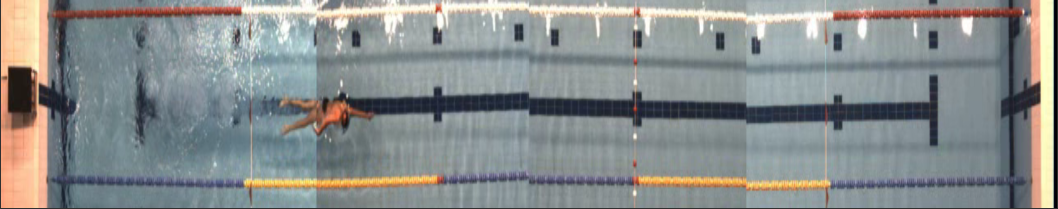
\includegraphics[width=\textwidth,height=\textheight,keepaspectratio]{imagenes/parte_IA/416x2112_YOLO_resize.png}
    \caption{Redimensión de una calle de la piscina para que tenga doble de alto.}
    \label{fig:ejemplredimensiondoblealto}
\end{figure}

Sin embargo, se decidió utilizar un tamaño de 256x2688 para redimensionar los fotogramas de los vídeos conforme entran a la red neuronal, dado que consideramos que es la combinación de valores que proporciona la mejor relación entre precisión en la predicción y tiempo de ejecución. Respecto del caso con dimensiones 416x2112 se obtuvieron valores del índice de Jaccard y Sorensen-Dice 0.001 y 0.015 menores, respectivamente. Esta pequeña diferencia no es prácticamente apreciable, ya que para valores del índice de Jaccard cercanos a 0.7 las predicciones son bastante buenas, pero gracias a ella se consigue una considerable mejora en el tiempo de ejecución del 19.14\%.

Tras evaluar el rendimiento del modelo basado en técnicas de aprendizaje profundo, compararemos el mismo con el modelo propuesto en el capítulo \ref{cap:capitulo3}. 

En la figura \ref{fig:iouvisualimgsyolo} se pueden observar seis fotogramas, que representan distintas condiciones de detección. Se remarcan en rojo las predicciones realizadas por el modelo basado en técnicas de aprendizaje profundo propuesto en este capítulo.

\begin{figure}[h!]
    \centering
    \begin{tabular}{cc}
          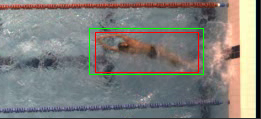
\includegraphics[width=0.43\textwidth,height=0.43\textheight,keepaspectratio]{imagenes/parte_IA/iou_visual/1099_recortada.png} &
          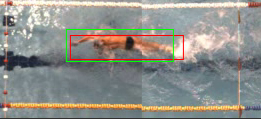
\includegraphics[width=0.43\textwidth,height=0.43\textheight,keepaspectratio]{imagenes/parte_IA/iou_visual/1259_recortada.png}
          \\ Fotograma A   & Fotograma B \\
          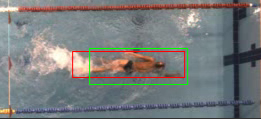
\includegraphics[width=0.43\textwidth,height=0.43\textheight,keepaspectratio]{imagenes/parte_IA/iou_visual/1014_recortada.png} &
          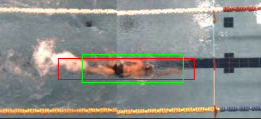
\includegraphics[width=0.43\textwidth,height=0.43\textheight,keepaspectratio]{imagenes/parte_IA/iou_visual/897_recortada.png}
          \\ Fotograma C & Fotograma D \\
          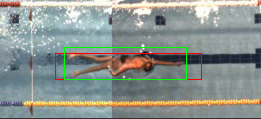
\includegraphics[width=0.43\textwidth,height=0.43\textheight,keepaspectratio]{imagenes/parte_IA/iou_visual/611_recortada.png} &
          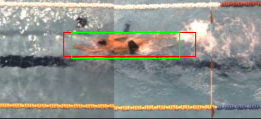
\includegraphics[width=0.43\textwidth,height=0.43\textheight,keepaspectratio]{imagenes/parte_IA/iou_visual/1241_recortada.png}
          \\Fotograma E & Fotograma F
     \end{tabular}
     \caption{Predicción automática (en rojo) frente a segmentación manual (en verde) para varios fotogramas.}
     \label{fig:iouvisualimgsyolo}
\end{figure}

\begin{table}[]
    \centering
    \begin{tabular}{| c | c | c | } \hline
        Fotograma & IoU & Sorensen-Dice \\ \hline
        A & 0.78566 & 0.87997  \\
        B & 0.67467 & 0.80574 \\   
        C & 0.62217 & 0.76708 \\ 
        D & 0.59528 & 0.74631 \\ 
        E & 0.70053 & 0.82390 \\ 
        F & 0.76596 & 0.86747 \\ \hline
    \end{tabular}
    \caption{Métricas para predicciones frente a segmentación manual para varios fotogramas.}
    \label{tab:iouvisualtabyolo}
\end{table}

Como se puede apreciar, YOLOv4 es capaz de identificar al nadador en su totalidad en todos los fotogramas, mientras que el enfoque del capítulo \ref{cap:capitulo3} genera predicciones en las que sólo se reconoce el tronco superior del nadador. También se puede observar cómo las predicciones de YOLO tienden a incluir parte del agua en la bounding box que contiene al nadador, aunque reducen considerablemente la cantidad de agua detectada como parte del nadador en fotogramas en los que existen un gran chapoteo.

En la tabla \ref{tab:iouvisualtabyolo} se pueden observar los valores de los índices de Jaccard y Sorensen-Dice para las predicciones presentadas en la figura \ref{fig:iouvisualimgsyolo}. Todos los fotogramas presentan un valor IoU superior a 0.6, a partir del cual podemos considerar las predicciones como acertadas, teniendo 4 de los 6 fotogramas un valor superior a 0.67. Si se comparan estos valores con los presentados en la tabla \ref{tab:iouvisualtab} para la aproximación del capítulo \ref{cap:capitulo3}, se observa una mejora sustancial para los tres primeros fotogramas y una ligera disminución de la precisión de la predicción para los dos últimos fotogramas.

Tras haber ejemplificado las diferencias entre los enfoques para seis fotogramas concretos, abordemos los resultados medios obtenidos para los 45 fotogramas utilizados en el conjunto de pruebas. En la tabla \ref{tab:metricasaproximaciones} se muestran los valores medios de los índices de Jaccard y Sorensen-Dice, así como el tiempo medio de procesamiento por fotograma para ambos enfoques. 

\begin{table}[]
    \centering
    \begin{tabular}{| c | c | c | c | } \hline
        Enfoque & IoU & F1Score  & T.ejecución (ms)  \\ \hline
        GSoC sobre Cr & 0.64126 & 0.76864 & \textbf{11.051} \\
        YOLOv4 & \textbf{0.72532} & \textbf{0.82767} & 54.571  \\ \hline
    \end{tabular}
    \caption{Métricas para cada aproximación.}
    \label{tab:metricasaproximaciones}
\end{table}

Como se podía intuir, YOLO obtiene métricas mejores que el modelo propuesto en el capítulo \ref{cap:capitulo3}. Esto se debe principalmente a dos factores:
\begin{enumerate}
    \item YOLO es capaz de detectar al nadador completo donde la aproximación del capítulo anterior sólo detecta modo el tronco del nadador.
    \item YOLO reduce en gran medida la cantidad de agua reconocida como parte del nadador en fotogramas donde existe un gran chapoteo, aunque tiende a incluir de manera general un poco de agua en las bounding box de las predicciones.
\end{enumerate}

En contraposición, el modelo basado en técnicas de aprendizaje profundo requiere de un tiempo de procesamiento considerable, dado que es 4.94 veces más lento que el enfoque propuesto en el capítulo \ref{cap:capitulo3}. 

Tras analizar el rendimiento del método basado en aprendizaje profundo, y compararlo con el rendimiento ofrecido por el modelo propuesto en el capítulo \ref{cap:capitulo3}, en el capítulo \ref{cap:capitulo5} se detallará el método que se utilizará para calcular la frecuencia media de nado y se decidirá que algoritmo de detección de objetos ofrece mejores resultados.


	\chapter{Cálculo de la frecuencia media de nado} \label{cap:capitulo5}

En los capítulos anteriores hemos presentado dos métodos para detectar al nadador a lo largo de su recorrido por la piscina. Estos métodos devuelven una bounding box que contiene al nadador en cada fotograma.

En este capítulo propondremos un modelo para calcular la frecuencia media de nado (FMN)(en brazadas por minuto) a partir de las bounding boxes obtenidas. Para ello, necesitaremos estimar: (i) cuánto tiempo se tarda en recorrer cada tramo de la piscina (split) y (ii), cuántas brazadas se han realizado en cada tramo.

Para estimar la FMN, haremos uso de la información que nos proporcionan las bounding boxes, concretamente, la coordenada X y la anchura vertical. Estos valores necesitan de un preprocesamiento, que describimos en la sección \ref{sec:preprocessdata}. Posteriormente, en las secciones \ref{calculotiemposplit} y \ref{sec:brazadassplit} utilizaremos la información procesada para calcular el tiempo empleado y las brazadas por split, respectivamente. Finalmente, en la sección \ref{sec:resultadoscalculos} se realiza una comparativa entre los métodos de detección del nadador basados en técnicas clásicas, (capítulo \ref{cap:capitulo3}), y redes neuronales, (capítulo \ref{cap:capitulo4}), para ver cual de ellos realiza una mejor estimación de la FMN en función de los cuatro estilos básicos de la natación. Estos estilos de nado son crol, mariposa, braza y espalda

\section{Preprocesado de los coordenadas y anchuras de las bounding boxes} \label{sec:preprocessdata}

Los métodos de detección presentados en los capítulos \ref{cap:capitulo3} y \ref{cap:capitulo4} realizan detecciones del nadador bastante precisas en cada fotograma. Sin embargo, la información que proporcionan puede contener: (i) valores nulos en aquellos fotogramas donde no se detecto al nadador, dado que no se dispone bounding box de la que extraer la información, o (ii) ruido derivado de una variación imprevista de los valores, por lo que es necesario procesar estos datos para evitar estos inconvenientes.

Para evitar tener huecos o variaciones muy pronunciadas en la función que describen los valores de la coordenada X y anchura vertical de la caja, y dado que los nadadores avanzan de forma continua, en los fotogramas donde la detección falla, se asignan los valores de la bounding box detectada en el fotograma inmediatamente anterior.

Además, el proceso de detección tiene cierta imprecisión que produce ruido en las medidas de la bounding box y dificulta las estimaciones que necesitamos. Sabemos también que los valores de la bounding box no van a variar de forma brusca, y podemos por tanto utilizar técnicas de suavizado de datos para facilitar que las variaciones de la bounding box sigan una tendencia clara. 

Para realizar el suavizado se utiliza el ``filtro de Savitzky–Golay'', descrito por primera vez en 1964 por Abraham Savitzky y Marcel J. E. Golay en el artículo \cite{filtrosavgol}, y cuya implementación se encuentra disponible en el paquete software \textit{Scipy}. El método se basa en el cálculo de una regresión polinomial local mediante puntos equi-espaciados. Dado que el objetivo de este trabajo no es analizar los cálculos realizados por el filtro, se invita al lector interesado a consultar el artículo anteriormente citado.

Se usa este filtro dado que la función suavizada generada tiende a mantener las características de la distribución inicial, tales como extremos relativos y anchura de los mismos \cite{filtrosavgol}. Esto es de especial relevancia dado que se hará uso de los extremos relativos para identificar los momentos en los que se cambia el sentido del nado y en los que se realiza una brazada. Si se desvirtuaran los extremos relativos podríamos incurrir en imprecisiones en los cálculos.

\section{Cálculo del tiempo empleado por split} \label{calculotiemposplit} 

En esta sección abordaremos cómo calcular el tiempo que tarda en recorrerse cada split, ya que necesitaremos de esta información para poder calcular la frecuencia media de nado, tanto por split como para la secuencia de vídeo en su totalidad. 

Como se mencionaba en el capítulo \ref{cap:capitulo2}, sólo estamos interesados en lo que ocurre en unas determinadas regiones de interés (ROI) dentro de cada split. En el primer split, es necesario ignorar el salto con el que el nadador entra a la piscina. En split sucesivos, es necesario ignorar la voltereta que el nadador da para cambiar de sentido e impulsare en la pared de la piscina. Por tanto, la ROI es una zona delimitada del split que ignora los extremos. 

En la figura \ref{fig:limitesroi} se muestran los límites de las ROIs. Nótese que las coordenadas de estos límites son conocidas, puesto que el sistema de captación de vídeo es fijo.

\begin{figure}
    \centering
    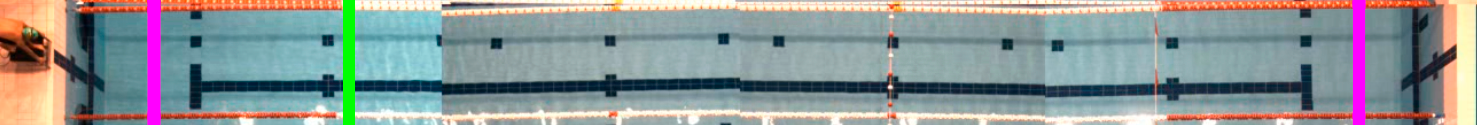
\includegraphics[width=\textwidth,height=\textheight,keepaspectratio]{imagenes/parte_graficas/limites_ROI.png}
    \caption{Límites de la región de interés. En verde se marca el inicio de la primera ROI, en morado se marcan los límites habituales para las ROI.}
    \label{fig:limitesroi}
\end{figure}

Utilizaremos la coordenada X de la esquina inferior izquierda de la bounding para distinguir el sentido de nado del nadador. Cuando el valor siga una tendencia creciente sabremos que se esta nadando de izquierda a derecha, mientras que si la tendencia es decreciente se estará nadando en el sentido contrario.

En la figura \ref{fig:diagramasecuenciacoordenadasX} se puede observar un diagrama de secuencia que resume el procedimiento que vamos a seguir. Nótese que los dos primeros pasos corresponden al preprocesamiento descrito en la sección anterior.

\begin{figure}
    \centering
    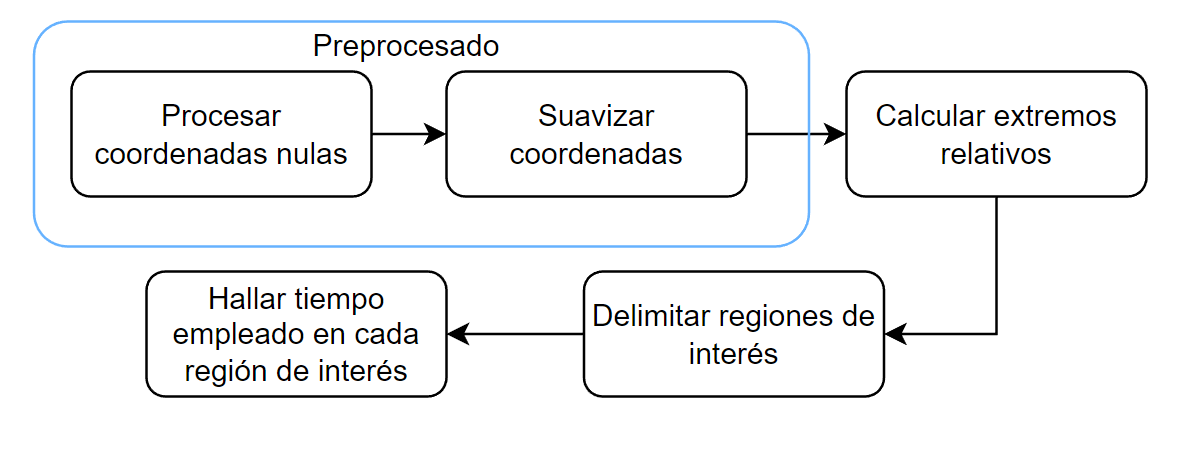
\includegraphics[width=\textwidth,height=\textheight,keepaspectratio]{imagenes/parte_graficas/Coordenada X.png}
    \caption{Secuencia de procesado de las coordenada X.}
    \label{fig:diagramasecuenciacoordenadasX}
\end{figure}

Tras haber realizado el preprocesamiento de las coordenadas X, hallaremos los extremos relativos de la función que describen. Los extremos relativos nos permiten identificar los momentos en los que el nadador cambia el sentido del nado, y por tanto se cambia de split, ya que el valor de las coordenadas X cambia de tendencia. Para ello, haremos uso de la función \textit{find\_peaks} del paquete software \textit{Scipy}. Esta función nos permite obtener los máximos relativos de una función, pero no los mínimos relativos. Para resolver este inconveniente se utiliza esta función dos veces; la primera de ellas se realiza sobre la distribución suavizada para obtener sus máximos relativos, mientras que la segunda vez se utiliza sobre la distribución suavizada multiplicada por menos uno. Los máximos relativos de la distribución cambiada de signo equivalen a los mínimos relativos de la distribución original. 

En la figura \ref{fig:ejemplocoordenadasX} se puede apreciar la evolución de la coordenada X de la esquina inferior izquierda de la bounding box. En dicha gráfica se han marcado los principales puntos de interés. Los puntos verdes indican los límites de cada split, mientras que los puntos azules indican los límites de cada región de interés. En torno al fotograma 800 se encuentra el máximo absoluto que indica el cambio de sentido de nado. 


\begin{figure}
   \centering
   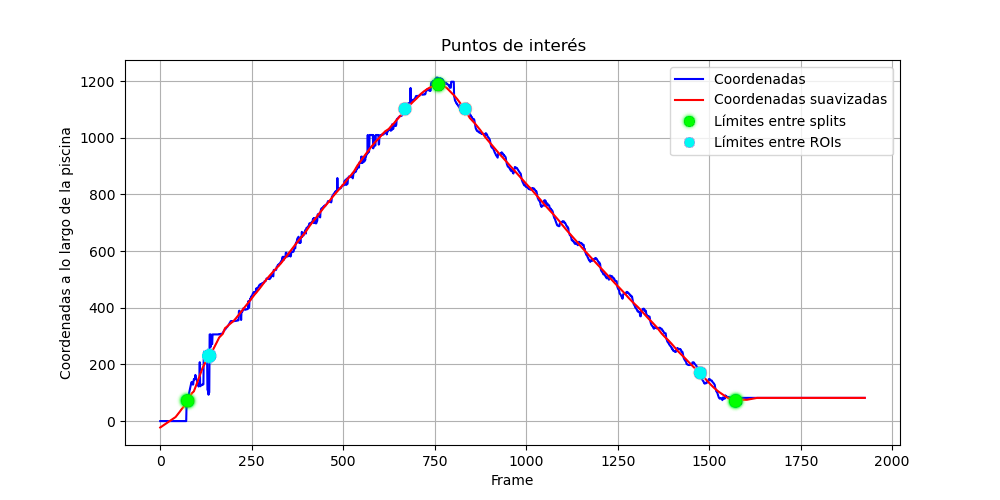
\includegraphics[width=\textwidth,height=\textheight,keepaspectratio]{imagenes/parte_graficas/SENTID.png}
   \caption{Evolución de la coordenada X y puntos de interés.}
   \label{fig:ejemplocoordenadasX}
\end{figure}

Conocidos los extremos relativos del conjunto de valores correspondientes a la coordenada X en que se encuentra el nadador, se utilizará el número de fotograma en que se producen para delimitar los splits. De esta manera, un split durará el número de fotogramas que separe un máximo y mínimo relativo consecutivos.

Esto permite delimitar los splits en los que se divide la prueba, a excepción del primero y el último. Dichos splits deben ser tratados de forma especial dado que no se pueden obtener gracias a la distancia de extremos relativos; esto es debido a que: (i) cuando se inicia el primer split los valores de la coordenada X siguen una tendencia estrictamente creciente, por lo que no existe mínimo relativo, (ii) cuando se termina el último split los valores siguen una tendencia estrictamente decreciente, por lo que no existe máximo relativo.

Para calcular el tiempo que se tarda en recorrer la región de interés en cada uno de los split delimitados, haremos uso de los números de fotograma en los que el nadador pasa por los extremos de la región de interés, cuyas posiciones son constantes y conocidas. Conocidos los fotogramas límite de las regiones de interés (ROI), hallar el tiempo empleado para recorrerlas será tan sencillo como aplicar la expresión: 

\begin{equation}
    T (s) = \frac{\text{nº fotograma final ROI} - \text{nº fotograma inicial ROI}}{ \text{tasa de fotogramas por segundo}}
\end{equation}

Tras haber delimitado las regiones de interés de cada split y haber calculado el tiempo que se tarda en recorrerlas, se debe proceder a calcular el número de brazadas que tiene lugar en cada región.

\section{Detección de brazadas y cálculo de la frecuencia media de nado} \label{sec:brazadassplit}

Como se introdujo en el capítulo \ref{cap:capitulo2}, el movimiento realizado por los brazos del nadador sigue una cierta periodicidad. Por tanto, podemos estimar el número de brazadas a partir de la variación en la anchura en el eje Y de la caja que proporcionan los métodos de detección utilizados en los capítulos anteriores. Las brazadas corresponderán a fotogramas en los que la anchura de la caja en el eje Y sea máxima, dado que el nadador debe extender los brazos hacia los lados para bracear. Este comportamiento se puede apreciar  en la figura \ref{fig:vervariacionanchura}. En dicha figura se puede apreciar claramente cómo la anchura de la caja en el eje Y aumenta conforme se extienden los brazos para realizar la brazada, y disminuye tras realizarla para volver a la posición inicial, por lo que podemos usar el momento de máxima anchura para reconocer la realización de la brazada. Este comportamiento se repite de forma periódica. Nótese que la variación de anchura concreta dependerá del estilo de nado, pero todos ellos comparten la tendencia mencionada.

\begin{figure}
    \centering
    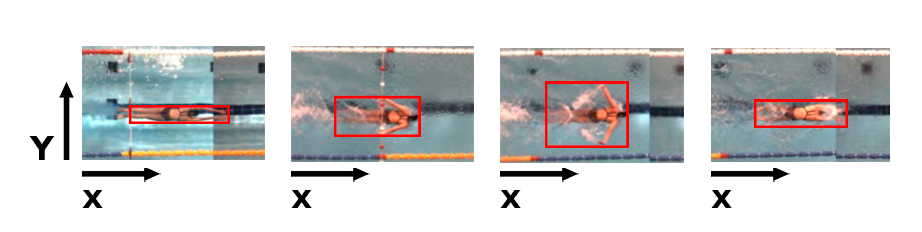
\includegraphics[width=\textwidth,height=\textheight,keepaspectratio]{imagenes/parte_graficas/variacion_anchura_nadador.png}
    \caption{Variación de anchura de la caja del nadador en el eje Y conforme se realiza una brazada.}
    \label{fig:vervariacionanchura}
\end{figure}

En la figura \ref{fig:diagramasecuenciaanchura} se muestra un diagrama de secuencia del procesado que se va a realizar sobre las anchuras del nadador en cada fotograma del vídeo, obtenidas con los métodos de detección de los capítulos \ref{cap:capitulo3} y \ref{cap:capitulo4}.

\begin{figure}
    \centering
    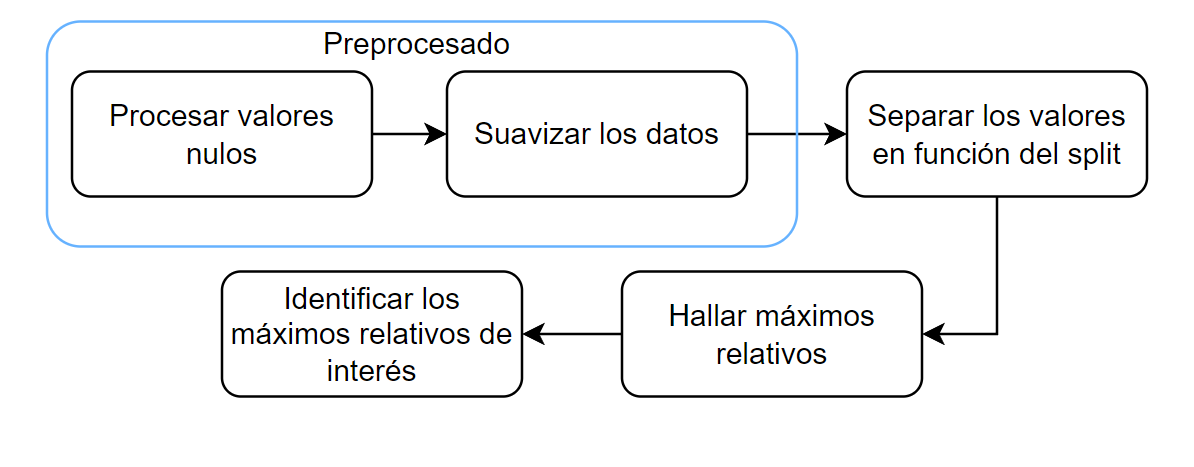
\includegraphics[width=\textwidth,height=\textheight,keepaspectratio]{imagenes/parte_graficas/Anchura.png}
    \caption{Secuencia de procesado de las anchuras de los nadadores.}
    \label{fig:diagramasecuenciaanchura}
\end{figure}

Tras haber preprocesado las anchura de las cajas, hallaremos los máximos relativos utilizando la función \textit{find\_peaks}. Sin embargo, no todos los máximos relativos nos serán de interés, pues no todos ellos corresponderán a brazadas del nadador. 

Los máximos relativos que permitirán distinguir las brazadas son aquellos de mayor valor. La función \textit{find\_peaks} permite discriminar aquellos menos relevantes e ignorarlos. Adicionalmente, impondremos la condición de que un máximo relativo pueda ser candidato a brazada sí tiene un valor mayor a la media del conjunto de valores. Este criterio se basa en el hecho de que en la mayoría de técnicas de nado los momentos de braceo son menores y de menor duración que aquellos en los que el brazo se encuentra estirado horizontalmente, con una menor anchura.

Por último, se considerarán como brazadas aquellos máximos relativos que se distancian entre sí en un determinado número mínimo de fotogramas. Esta distancia entre fotogramas es un parámetro clave, dado que permitirá obviar situaciones imposibles de realizar por un nadador, como bracear dos veces en menos de 0.2 segundos. La distancia mínima entre fotogramas utilizada para realizar esta selección es igual a la mitad de la tasa de fotogramas por segundo. Este valor fue proporcionado por los investigadores de la Facultad de Ciencias del Deporte, basándose en que ninguno de sus nadadores es capaz de realizar dos brazadas consecutivas en menos de medio segundo. 

Como se puede observar en las figuras \ref{fig:anchurasmariposa} y \ref{fig:anchurascrol}, correspondientes a nado en estilo mariposa y crol, el método propuesto permite distinguir las brazadas de una forma adecuada. También se puede apreciar cómo existen diferencias en las anchuras determinadas por los distintos detectores de objetos, existiendo un mayor nivel de ruido en las medidas obtenidas haciendo uso de GSoC. El análisis de la bondad de las predicciones realizadas con cada técnica de detección de objetos se pospone a la sección \ref{sec:resultadoscalculos}.

\begin{figure}
    \centering
    \begin{tabular}{c}
        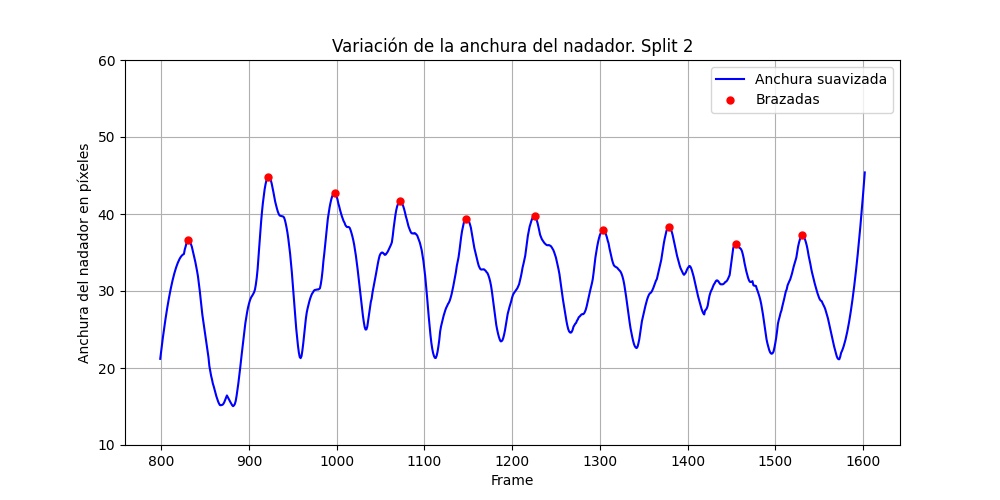
\includegraphics[width=0.6\textwidth,height=\textheight,keepaspectratio]{imagenes/parte_graficas/anchuras_calle_3_mariposa_GSoC.png}  \\
        a) Detección con GSoC. \\
         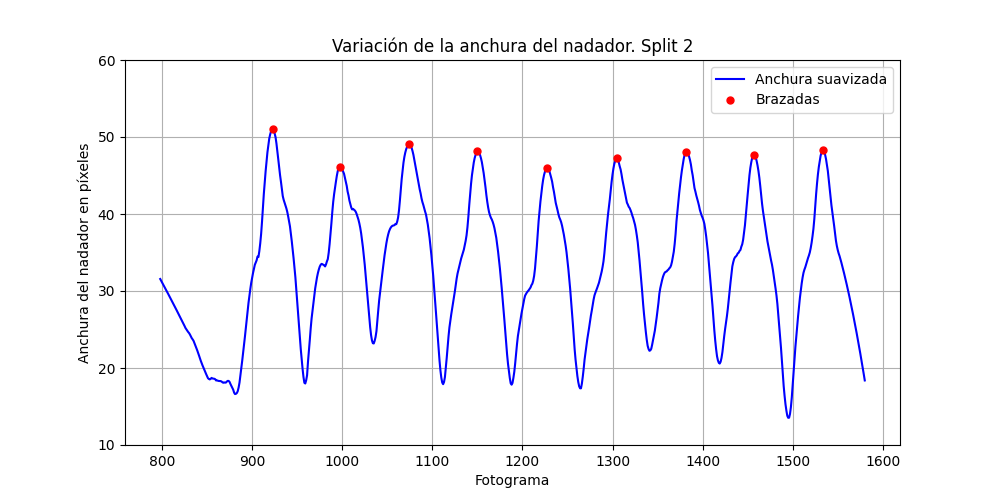
\includegraphics[width=0.6\textwidth,height=\textheight,keepaspectratio]{imagenes/parte_graficas/anchuras_calle_3_mariposa_YOLO.png} \\
        b) Detección con YOLO.
    \end{tabular}
    \caption{Anchuras para nado en mariposa.} % Split 2 calle 3.
    \label{fig:anchurasmariposa}
\end{figure}

    \begin{figure}
        \centering
        \begin{tabular}{c}
            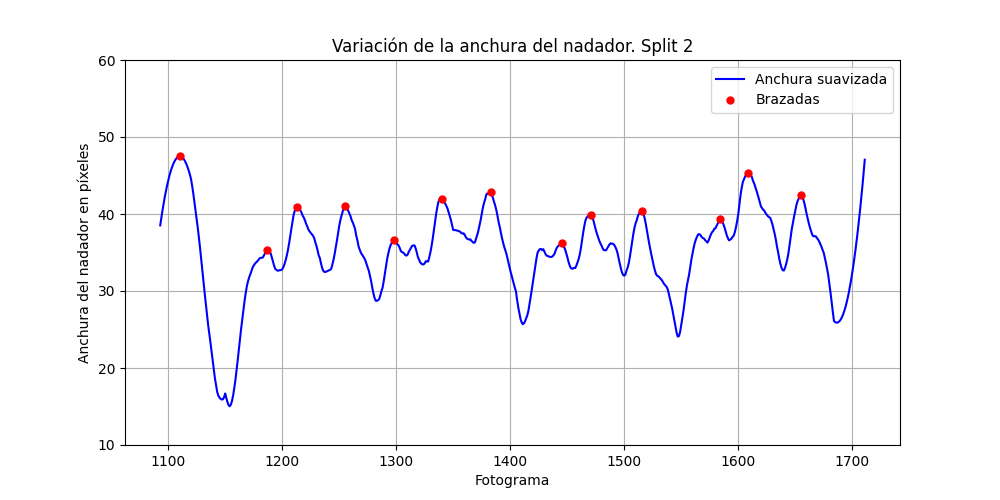
\includegraphics[width=0.6\textwidth,height=\textheight,keepaspectratio]{imagenes/parte_graficas/anchuras_calle_5_freestyle_GSoC.png}  \\
            a) Detección con GSoC. \\
             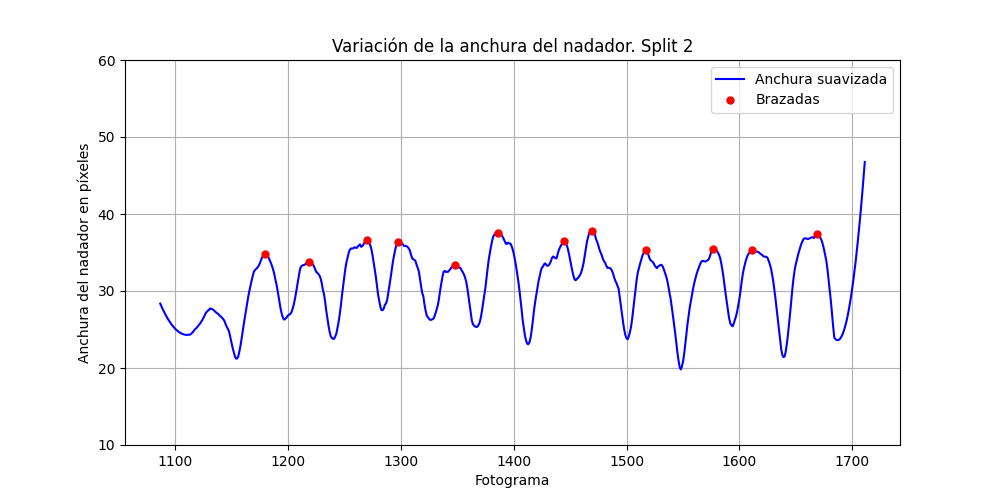
\includegraphics[width=0.6\textwidth,height=\textheight,keepaspectratio]{imagenes/parte_graficas/anchuras_calle_5_freestyle_YOLO.png} \\
            b) Detección con YOLO.
        \end{tabular}
        \caption{Anchuras para nado en crol.} % Split 2 calle 5.
        \label{fig:anchurascrol}
    \end{figure}


Una vez se conoce el tiempo que se tarda en recorrer cada región de interés, y el número de brazadas que se realiza en cada una de ellas, el cálculo de la frecuencia media de nado por split (FNMS) se reduce a:
\begin{equation}
    \text{FNMS} (brazadas/min) = \frac{ \text{número de brazadas} * \frac{\text{60 segundos}}{minuto} }{ \text{segundos en recorrer la región de interés}}
\end{equation}

Para calcular la frecuencia media de nado a lo largo de toda la prueba, bastará con calcular la media aritmética de los valores obtenidos anteriormente.

Tras haber descrito cómo calcular la frecuencia media de nado, tanto por split como para el total de la secuencia de vídeo. En la siguiente sección se mostrarán los resultados experimentales obtenidos.

\section{Evaluación experimental} \label{sec:resultadoscalculos}

Una vez que hemos presentado el modelo para el cálculo de la frecuencia media de nado analizaremos los resultados experimentales obtenidos. Para ello, vamos a comparar los datos obtenidos con cada aproximación (tiempo empleado en recorrer la región y número de brazadas) y el resultado final obtenido (FNMS).

Dado que los vídeos proporcionados por los investigadores de la Facultad de Ciencias del Deporte carecen de etiquetas, ha sido necesario etiquetarlos para realizar esta evaluación experimental. Se ha medido manualmente el tiempo que se tarda en recorrer las regiones de interés y el número de brazadas en 7 pruebas de 50 metros, de manera que tenemos 14 splits. Dado que existen diferentes estilos de nado, se han considerado dos pruebas de nado en estilo mariposa, dos en crol, dos en braza y una en espalda. Nótese que pese a que no se trata de un problema difícil, las etiquetas no provienen de un experto. 

\subsection{Estimación del tiempo empleado en recorrer una región de interés}
En primer lugar, se analizará la influencia del método de detección de objetos utilizado a la hora de realizar la estimación del tiempo que se tarda en recorrer cada región de interés.

Los tiempos estimados por cada una de las aproximaciones de los capítulos \ref{cap:capitulo3} y \ref{cap:capitulo4}, así como los tiempos reales para cada una de las pruebas se muestran en la tabla \ref{tab:tablatiemposcap5}. Todos ellos se encuentran expresados en segundos.

\begin{table}[]
    \centering
    \small
    \begin{tabular}{|c|c|c|c|} \hline
         Estilo & T. est. GSoC & T. est. YOLO & T. real  \\ \hline  
         Mariposa & 14.50 & 14.98 & 13.91  \\   
         Mariposa & 18.05 & 18.38 & 18.31 \\    
         Mariposa & 16.86 & 16.52 & 16.68 \\    
         Mariposa & 19.79 & 20.76 & 20.44 \\    
         Crol & 12.57 & 11.29 & 11.94  \\      
         Crol & 14.60 & 13.29 & 13.54 \\        
         Crol & 12.98 & 12.21 & 12.01 \\       
         Crol & 14.38 & 14.86 & 14.78 \\        
         Braza & 13.50 & 12.83 & 12.58 \\       
         Braza & 14.60 & 14.71 & 15.30 \\      
         Braza & 11.98 & 12.48 & 12.21  \\      
         Braza & 14.19 & 14.19 & 14.72  \\      
         Espalda & 15.81 & 15.31 & 15.55 \\    
         Espalda & 17.48 & 17.50 & 17.82 \\ \hline 
    \end{tabular}
    \caption{Tiempo estimado (en segundos) en recorrer cada ROI según los distintos métodos.}
    \label{tab:tablatiemposcap5}
\end{table} 

En la tabla \ref{tab:tablatiemposcap5} se puede observar cómo en ningún caso se predice correctamente el tiempo necesario para recorrer cada una de la regiones de interés. Ambos métodos discrepan en el tiempo predicho salvo en una ocasión, y no existe un patrón claro que indique que un método u otro tiende a estimar más o menos tiempo en función del estilo de nado. 

Para poder determinar que método ofrece predicciones más fiables se ha calculado el error absoluto relativo para cada caso. El error absoluto relativo es una métrica que indica la calidad de una predicción \cite{estadistica}. Este se define cómo:

\begin{equation}
    Error_{\text{absoluto relativo}} = \frac{|Valor_{real} - Valor_{predicho}|}{Valor_{real}}
\end{equation}

Utilizaremos esta métrica ya que nos indica la proporción del error con respecto al valor exacto de la medición, permitiéndonos comparar los errores que se producen en distintas pruebas. Nótese que no sería igual cometer un error de predicción de 2 segundos en una prueba de nado de 10 segundos, que en una prueba que durase una hora.

Esta información se puede consultar en la tabla \ref{tab:tablaerrorestiemposcap5}. Para obtener una visión más general en función del estilo de nado, se han calculado los errores relativos medios para cada uno de ellos, así como el error absoluto relativo medio total. Estos valores se pueden consultar en la tabla \ref{tab:tablatiemposmedioscap5}. Nótese que el error absoluto relativo es muy pequeño en todos los casos, por lo que ambas técnicas realizan una predicción del tiempo empleado en recorrer la ROI bastante precisa. Sin embargo, YOLO ofrece menor error absoluto relativo para todos los estilos de nado a excepción de mariposa, así como un menor error absoluto relativo  medio total. Por tanto, se puede concluir que YOLO ofrece mejores predicciones del tiempo que se tarda en recorrer cada región de interés.

\begin{table}[]
    \centering
    \small
    \begin{tabular}{|c|c|c|} \hline
         Estilo & Err. relatv. GSoC & Err. relatv. YOLO  \\ \hline 
         Mariposa & \textbf{0.04241} & 0.07692 \\
         Mariposa & 0.01420 & \textbf{0.00382} \\
         Mariposa & 0.01080 & \textbf{0.00959} \\
         Mariposa & 0.03180 & \textbf{0.01565} \\
         Crol & \textbf{0.05276} & 0.05444 \\
         Crol & 0.07829 & \textbf{0.01846} \\
         Crol & 0.08076 & \textbf{0.01665} \\
         Crol & 0.02706 & \textbf{0.00541} \\
         Braza & 0.07313 & \textbf{0.01987} \\
         Braza & 0.04575 & \textbf{0.03856} \\
         Braza & \textbf{0.01884} & 0.02211 \\
         Braza & 0.03600 & 0.03600 \\
         Espalda & 0.01672 & \textbf{0.01543} \\
         Espalda & 0.01908 & \textbf{0.01796} \\ \hline
    \end{tabular}
    \caption{Error absoluto relativo en las predicciones del tiempo empleado para recorrer cada ROI según los distintos métodos. }
    \label{tab:tablaerrorestiemposcap5}
\end{table}

\begin{table}[]
    \centering
    \small
    \begin{tabular}{|c|c|c|} \hline
         Estilo & Err. relatv. medio GSoC & Err. relatv. medio YOLO  \\ \hline
         Mariposa & \textbf{0.024803} & 0.026495 \\
         Crol & 0.061423 & \textbf{0.02374}  \\   
         Braza & 0.043430 & \textbf{0.029135} \\
         Espalda & 0.017900 & \textbf{0.016695} \\
         Media & 0.039603 & \textbf{0.025062} \\ \hline
    \end{tabular}
    \caption{Comparativa entre los errores relativos medios de los tiempos estimados.}
    \label{tab:tablatiemposmedioscap5}
\end{table} 

\subsection{Estimación del número de brazadas }
El número de brazadas estimado por cada una de las aproximaciones de los capítulos \ref{cap:capitulo3} y \ref{cap:capitulo4} se muestra en \ref{tab:tablabrazadascap5}.

\begin{table}[]
    \centering
    \small
    \begin{tabular}{|c|c|c|c|} \hline
         Estilo & Br. est. GSoC & Br. est. YOLO & Br. reales  \\ \hline
         Mariposa & 9 & 9 & 9  \\   
         Mariposa & 10 & 9 & 9 \\
         Mariposa & 11 & 11 & 11 \\
         Mariposa & 12 & 12 & 13 \\
         Crol & 8 & 8 & 8  \\
         Crol & 10 & 9 & 9 \\
         Crol & 9 & 11 & 11 \\  
         Crol & 13 & 12 & 12 \\
         Braza & 14 & 9 & 9 \\  
         Braza & 9 & 9 & 9 \\
         Braza & 9 & 10 & 10  \\
         Braza & 11 & 13 & 12  \\
         Espalda & 10 & 11 & 12 \\
         Espalda & 8 & 13 & 13 \\ \hline
    \end{tabular}
    \caption{Comparativa entre brazadas estimadas y reales.}
    \label{tab:tablabrazadascap5}
\end{table}


Analicemos los resultados presentados para cada estilo de nado. 
\begin{itemize}
    \item Para el nado en estilo crol, GSoC solamente es capaz de estimar el número de brazadas correcto en una ocasión. Para el segundo y cuarto caso estima una brazada de más, mientras que para el tercer caso estima dos brazadas menos. Sin embargo, se puede observar que YOLO es capaz de predecir correctamente el número de brazadas en todas las ocasiones.
    
    \item Para el nado en estilo mariposa, GSoC es capaz de estimar correctamente el número de brazadas realizadas en el primer y tercer caso, mientras que para el segundo caso estima una brazada de más y para el cuarto caso una brazada de menos. YOLO es capaz de predecir correctamente en tres de los cuatro casos analizados, estimando una brazada menos en el cuarto. Ambos métodos tienen dificultades para reconocer brazadas cuando estás se realizan muy cerca del final de la región de interés.
    
    \item Para el nado en braza, GSoC solamente es capaz de estimar correctamente en el segundo caso. Resulta especialmente notable el error cometido en el primer caso, donde se estiman 5 brazadas más de las realmente realizadas. Por otra parte, YOLO es capaz de acertar la predicción en los tres primeros casos, mientras que en el cuarto estima una brazada de más.
    
    \item Para el nado en espalda, GSoC no es capaz de acertar ninguna de las dos predicciones. Para el segundo caso, el error cometido es bastante notable, al estimar 5 brazadas menos de las realmente realizadas. YOLO es capaz de acertar la segunda predicción, mientras que en la primera estima una brazada de menos.
\end{itemize}

En la tabla \ref{tab:tablaerroresbrazadascap5} se muestra el error absoluto relativo cometido por cada aproximación a la hora de estimar el número de brazadas que tienen lugar en cada región de interés. Como se puede observar rápidamente, la aproximación propuesta en el capítulo \ref{cap:capitulo3} presenta un mayor error absoluto relativo que la aproximación propuesta en el capítulo \ref{cap:capitulo4} en la mayoría de casos donde no es capaz de acertar el número de brazadas realizadas. En la tabla \ref{tab:tablaerroresmediosbrazadas} se presentan los errores relativos medios en función del estilo de nado y el error absoluto relativo medio total. El detector YOLO ofrece un error absoluto relativo medio menor en todos los estilos de nado, siendo este capaz de no cometer ningún error a la hora de predecir brazadas en estilo crol. Nótese que el detector GSoC sufre especialmente a la hora de detectar brazadas del nadador en estilo braza y de espalda. 

\begin{table}[]
    \centering
    \small
    \begin{tabular}{|c|c|c|} \hline
         Estilo & Err. relatv. GSoC & Err. relatv. YOLO  \\ \hline 
         Mariposa & 0 & 0 \\
         Mariposa & 0.1111 & \textbf{0} \\
         Mariposa & 0 & 0 \\
         Mariposa & 0.0833 & 0.0833 \\
         Crol & 0 & 0 \\
         Crol & 0.1111 & \textbf{0} \\
         Crol & 0.1818 & \textbf{0} \\
         Crol & 0.0833 & \textbf{0} \\
         Braza & 0.5555 & \textbf{0} \\
         Braza & 0 & 0 \\
         Braza & 0.1000 & \textbf{0} \\
         Braza & 0.0833 & 0.0833 \\
         Espalda & 0.1666 & \textbf{0.0833} \\
         Espalda & 0.3846 & \textbf{0} \\ \hline
    \end{tabular}
    \caption{Error absoluto relativo en las predicciones del número de brazadas realizadas.} 
    \label{tab:tablaerroresbrazadascap5}
\end{table}

\begin{table}[]
    \centering
    \small
    \begin{tabular}{|c|c|c|} \hline
         Estilo & Err. relatv. medio GSoC & Err. relatv. medio YOLO  \\ \hline
         Mariposa & 0.0486 & \textbf{0.0208} \\
         Crol & 0.0941 & \textbf{0}  \\   
         Braza & 0.1847 & \textbf{0.0208} \\
         Espalda & 0.2765 & \textbf{0.0417} \\
         Media & 0.1330 & \textbf{0.0178} \\ \hline
    \end{tabular}
    \caption{Comparativa entre los errores relativos medios del número de brazadas estimadas.}
    \label{tab:tablaerroresmediosbrazadas}
\end{table} 

\subsection{Estimación de la frecuencia de nado media}

Una vez hemos comprobado la bondad en las estimaciones del tiempo que se emplea en recorrer un split y el número de brazadas realizadas, comprobamos que efecto tienen dichas estimaciones en el cálculo de la FNMS. A partir de los valores anteriores, en la tabla \ref{tab:frecuenciasmedianadoest} se muestran las frecuencias medias de nado estimadas y reales medidas en brazadas por minuto. Nótese que las frecuencias medias de nado reales han sido calculadas a partir de mediciones realizadas manualmente para cada vídeo, ya que los investigadores de la Facultad de Ciencias del Deporte no indicaron valores de referencia.

\begin{table}[]
    \centering
    \small
    \begin{tabular}{|c|c|c|c|} \hline
         Estilo & Est. GSoC & Est. YOLO & Valores reales  \\ \hline
         Mariposa & 37.24 & 36.06 & 38.82  \\   
         Mariposa & 33.25 & 29.38 & 29.49 \\
         Mariposa & 39.15 & 39.94 & 39.10 \\
         Mariposa & 36.39 & 34.68 & 38.16 \\
         Crol & 38.18 & 42.53 & 40.20  \\   
         Crol & 41.11 & 40.65 & 39.88 \\    
         Crol & 41.61 & 54.04 & 54.95 \\    
         Crol & 54.24 & 48.46 & 48.71 \\    
         Braza & 62.22 & 42.08 & 42.93 \\   
         Braza & 37.00 & 36.70 & 35.29 \\   
         Braza & 45.09 & 48.09 & 49.14  \\  
         Braza & 46.51 & 54.97 & 48.91  \\  
         Espalda & 37.95 & 43.11 & 46.30 \\ 
         Espalda & 27.47 & 44.57 & 43.77 \\ \hline 
    \end{tabular}
    \caption{Comparativa entre frecuencias medias de nado estimadas y reales.}
    \label{tab:frecuenciasmedianadoest}
\end{table}

En la tabla \ref{tab:tablaerroresprediccionesfrecuencia} se muestran los errores relativos para cada una de las pruebas evaluadas, remarcando en negrita el menor error absoluto relativo en cada caso. Por otra parte, en la tabla \ref{tab:tablaerroresmediosprediccionesfrecuencia} se muestran los errores relativos medios para cada uno de los estilos de nado, así como el error absoluto relativo medio total.

\begin{table}[]
    \centering
    \small
    \begin{tabular}{|c|c|c|} \hline
         Estilo & Err. relatv. GSoC & Err. relatv. YOLO  \\ \hline 
         Mariposa & \textbf{0.0407} & 0.0711 \\
         Mariposa & 0.1275 & \textbf{0.0031} \\
         Mariposa & \textbf{0.0013} & 0.0215 \\
         Mariposa & \textbf{0.0464} & 0.0912 \\
         Crol & \textbf{0.05024} & 0.05796 \\
         Crol & 0.03084 & \textbf{0.01931} \\
         Crol & 0.24277 & \textbf{0.01656} \\
         Crol & 0.11353 & \textbf{0.00513} \\
         Braza & 0.44933 & \textbf{0.01980} \\
         Braza & 0.04845 & \textbf{0.03995} \\
         Braza & 0.08302 & \textbf{0.02136} \\
         Braza & \textbf{0.04907} & 0.12390 \\
         Espalda & 0.18034 & \textbf{0.06889} \\
         Espalda & 0.37240 & \textbf{0.01827} \\ \hline
    \end{tabular}
    \caption{Error absoluto relativo en las predicciones de la frecuencia media de nado.}
    \label{tab:tablaerroresprediccionesfrecuencia}
\end{table}

\begin{table}[]
    \centering
    \small
    \begin{tabular}{|c|c|c|} \hline
         Estilo & Err. relatv. medio GSoC & Err. relatv. medio YOLO  \\ \hline
         Mariposa & 0.0540 & \textbf{0.0467} \\
         Crol & 0.1093 & \textbf{0.0247}  \\   
         Braza & 0.1574 & \textbf{0.0417} \\
         Espalda & 0.2764 & \textbf{0.0436} \\
         Media & 0.1311 & \textbf{0.0385} \\ \hline
    \end{tabular}
    \caption{Comparativa entre los errores relativos medios de las frecuencias medias de nado estimadas.}
    \label{tab:tablaerroresmediosprediccionesfrecuencia}
\end{table} 

Como se puede observar en la tabla \ref{tab:tablaerroresmediosprediccionesfrecuencia}, YOLO ofrece un menor error absoluto relativo medio en todas los estilos de nado. A excepción del estilo mariposa, YOLO ofrece una reducción bastante considerable de los errores relativos con respecto de GSoC. Se puede observar que el error absoluto relativo medio total de YOLO es unas 3.4 veces menor, aproximadamente. Esto es un indicativo de que las predicciones realizadas por YOLO se acercan más a la realidad que las realizadas por GSoC.

En virtud de los experimentos realizados, se puede concluir que el método propuesto es capaz de predecir con un buen nivel de acierto tanto el tiempo que se tarda en recorrer una región de interés como el número de brazadas que hicieron falta para ello, y por tanto, la frecuencia media de nado. En concreto, los experimentos indican que YOLO ofrece un rendimiento superior frente a GSoC al realizar la estimación de la frecuencia media de nado con nivel de error considerablemente menor.

	\chapter{Conclusiones y trabajo futuro} \label{cap:capitulo6}

\section{Conclusiones}

Este Trabajo Fin de Grado propone y analiza una primera aproximación a la estimación del cálculo de la frecuencia media de nado de nadadores en piscinas con sistemas de captación de vídeo, propuesta por investigadores de la Facultad de Ciencias del Deporte de la Universidad de Granada. 

La solución presentada consta de dos pasos: (i) detección del nadador, (ii) estimación de la frecuencia de nado. 

Para realizar la detección del nadador se propone el uso de técnicas clásicas del procesamiento de imágenes, entre las que se encuentran la correcta elección del espacio de color y el uso de algoritmos de sustracción de fondos y extracción de contornos; y técnicas basadas en aprendizaje automático y redes neuronales convolucionales orientadas a la detección de objetos, YOLO. 

Para realizar la estimación de la frecuencia de nado se necesita determinar el tiempo que se tarda en recorrer la región de interés para cada split y obtener el número de brazadas realizadas para cada región de interés.

Estos cálculos se realizan utilizando los parámetros de las cajas generadas por los métodos de detección. Mediante la posición en el eje X puede estimarse cuanto tarda el nadador en recorrer la región de interés. Dado que el nadador debe extender los brazos hacia los lados cuando bracea, el número de brazadas es determinado a partir de los momentos de máxima anchura en el eje Y de la caja que contiene al nadador.

Se ha comprobado experimentalmente que la solución propuesta permite calcular correctamente la frecuencia media de nado. Los mejores resultados, bastante fieles a la realidad, han sido obtenidos haciendo uso de aprendizaje profundo con la arquitectura de detección de objetos YOLOv4, con un error relativo de 0.0385 frente a 0.1311 de la aproximación clásica.

Además, extraemos las siguientes conclusiones:
\begin{itemize}
    \item El uso de YOLOv4, siempre que este haya sido entrenado con un conjunto de imágenes lo suficientemente representativo, permite realizar detecciones bastante precisas de la posición y contorno del nadador. Estas detecciones proporcionan información suficiente para realizar una estimación bastante precisa de la frecuencia de nado en la mayoría de situaciones.
    
    \item Las bandas de crominancia del espacio de color YCbCr proporcionan una cierta robustez frente a variaciones de iluminación, lo que facilita a los algoritmos de sustracción de fondos detectar al nadador sin incluir el agua que le rodea.
    
    El uso de la banda de crominancia roja de YCbCr y el algoritmo de sustracción de fondos GSoC es la combinación que mejores resultados proporciona de entre las probadas durante el tercer capítulo.
    Esta permite obtener una estimación de la frecuencia de nado aceptable para la mayoría de estilos de natación.
    
    \item Los datos proporcionados por las técnicas clásicas del procesamiento de imágenes suelen tener una mayor cantidad de ruido que los proporcionados por YOLOv4. Este ruido desvirtúa el carácter periódico de la variación de anchura del nada, lo que dificulta la detección de las brazadas. En consecuencia, YOLOv4 permite realizar una mejor estimación de la frecuencia media de nado que las técnicas clásicas del procesamiento de imágenes.
    
    \item El tiempo de cómputo requerido por YOLOv4 es significativamente mayor que el requerido por los algoritmos de sustracción de fondos. El uso de esta arquitectura de aprendizaje profundo requiere de un hardware más potente que el que requieren las técnicas clásicas. En función del hardware utilizado, el tiempo requerido por YOLOv4 puede no ser siempre asumible. 
    
\end{itemize}

\section{Trabajo futuro}

El presente trabajo propone una primera aproximación a la estimación del cálculo de la frecuencia media de nado de nadadores, la cual resulta prometedora. Sin embargo, somos conscientes de que esta se ha probado con un conjunto reducido de vídeos, por lo que sería necesario validar el modelo con más ejemplos. Así pues, creemos que esta solución puede ser mejorada en un futuro. A continuación, se plantean varias líneas que consideramos de interés para futuros trabajos.

\begin{itemize}
    \item Los algoritmos de sustracción de fondos analizados en este trabajo presentan problemas a la hora de obviar el chapoteo del agua, ya que el valor de dichos píxeles cambia muy frecuentemente. El uso de nuevos algoritmos de sustracción de fondos que minimicen la detección de píxeles intermitentes podría mejorar los resultados obtenidos.  
    
    \item En este trabajo se ha hecho uso de YOLOv4, sin embargo existen nuevas versiones de esta arquitectura de detección de objetos. El uso de nuevas versiones podría contribuir a una mejora en los resultados obtenidos y/o a una reducción del tiempo de cómputo necesario. No obstante, el uso de arquitecturas más complejas puede conllevar requisitos de hardware más costosos.
    
    Un conjunto de imágenes de entrenamiento más variado podría mejorar considerablemente los resultados obtenidos, especialmente para nado en braza, ya que no disponíamos de imágenes de entrenamiento para dicho estilo de nado. Además, el uso de imágenes de entrenamiento similares en dimensiones a los fotogramas de los vídeos donde se realizaría la detección podría contribuir a una mejora de los tiempos de ejecución, dado que las resoluciones de entrada a la red podrían ser menores. Estos tiempos podrían ser reducidos aún más si se utilizan máquinas que cuenten con tarjetas gráficas de última generación.
    
    \item El uso de técnicas clásicas del procesamiento de imágenes y técnicas basadas en aprendizaje profundo no es excluyente. Dado que el uso de las bandas de crominancia del espacio de color YCbCr permite reducir la influencia de las variaciones de iluminación y del chapoteo generado en el agua, creemos que el uso de estas a la hora de utilizar una arquitectura de detección de objetos como YOLO permitiría mejorar los resultados obtenidos en este trabajo. 

    \item En este trabajo se ha propuesto un modelo de cálculo de la frecuencia media de nado común para diferentes estilos de nado. Con un número de ejemplos mayor se podrían desarrollar variaciones del método propuesto para cada estilo de nado, de manera que se tuvieran más en cuenta las particularidades de cada uno de ellos y se obtuvieran mejores resultados.
\end{itemize}

	
	\chapter*{Anexo I} \label{anexo1}

Detallamos en este anexo las herramientas de software y hardware que se han utilizado.

Para poder desarrollar este trabajo se ha utilizado el paquete software \textit{OpenCV}, que proporciona la inmensa mayoría de herramientas que se necesitarán, tales como lectura de vídeos, conversión entre espacios de color, algoritmos de sustracción de fondos y extracción de contornos y algoritmos de detección de objetos mediante redes neuronales profundas. También se usará la librería \textit{Scipy} para realizar diversos cálculos estadísticos y el paquete \textit{Matplotlib} para generar gráficas. Como lenguaje de programación se ha decidido utilizar \textit{Python}, que permite manejar y analizar los datos extraídos de forma sencilla y cómoda. 

Los requisitos necesarios para ejecutar el software desarrollado se listan a continuación:
\begin{itemize}
    \item Python 3.7 o superior.
    \item OpenCV 4.0 o superior. Dado que se necesita habilitar el soporte con CUDA y cudNN, la instalación deberá ser realizada a partir del código fuente disponible en el repositorio de Github \cite{repoopencvi}. Además, dado que se utilizan algoritmos de sustracción de fondos presentes en los módulos extra, debe usarse también el código fuente del repositorio \cite{repoopencvii} a la hora de construir e instalar el paquete.
    \item Scipy 1.2.0 o superior.
    \item Matplotlib.
    \item CUDA 10.2 o superior y cuDNN 8.0.2 o superior.
    \item Tarjeta gráfica NVIDIA con soporte para CUDA y cuDNN con un mínimo de 4 GB de memoria VRAM.
\end{itemize}

El código fuente desarrollado en el marco de este proyecto se encuentra publicado como software libre en el repositorio \cite{myownrepo}. Este trabajo ha sido desarrollado gracias al material proporcionado por investigadores de la facultad de Ciencias del Deporte. Sin embargo, dado que no se ha recibido autorización expresa por parte de los mismos para la difusión del material, este no es adjuntado en la entrega ni se encuentra disponible en el repositorio de Github.

Adicionalmente, para el entrenamiento de la red neuronal, se ha hecho uso del software \textit{Darknet}, disponible en \cite{darknetgithub}, el cual requiere a su vez de una tarjeta gráfica \textit{NVIDIA} con soporte para las plataformas de cómputo \textit{CUDA} y \textit{cuDNN}. Los requisitos mínimos de este software se listan a continuación:
\begin{itemize}
    \item CMake 3.18 o superior.
    \item OpenCV 2.4 o superior.
    \item CUDA 10.2 o superior y cuDNN 8.0.2 o superior.
    \item Una tarjeta gráfica NVIDIA con soporte para CUDA y cuDNN con capacidad de cómputo superior a 3.0. El valor de este índice se puede consultar en la página oficial de NVIDIA.
\end{itemize}
Adicionalmente, el autor del repositorio recomienda el uso de tarjetas gráficas con más de 10 GB de memoria VRAM.




	\thispagestyle{empty}
	\chapter*{Anexo II} \label{anexo2}

En este apéndice se detalla un experimento adicional que se realizó, pero que finalmente no se considera relevante.

La bondad de las estimaciones del tiempo que se tarda en recorrer una región de interés y el número de brazadas que se necesita para ello depende en gran medida del ruido existente en las distribuciones de datos usadas. Para determinar cual de los métodos propuestos en los capítulos \ref{cap:capitulo3} y \ref{cap:capitulo4} genera un menor nivel de ruido se ha calculado la desviación típica de la diferencia de valores de la coordenada X y anchura de la caja fotograma a fotograma. Puesto que esperamos obtener funciones suaves, el valor en un fotograma debe ser similar al anterior, y por tanto las diferencias deben ser cercanas a cero.

La desviación típica es una medida estadística utilizada para cuantificar la variación de un conjunto de datos numéricos. Un valor bajo indica que la mayor parte de los datos de la muestra tienen un valor cercano a la media, mientras que un valor alto de este índice implica que los datos se extienden sobre un rango de valores más amplio \cite{estadistica}. Así, proporcionará datos con menor ruido, y más estables conforme avancen los fotogramas, aquel método que tenga una menor desviación típica. 

En la tabla \ref{tab:desviaciondiferenciasX} se muestran la media de las desviaciones típicas para la diferencia de coordenada X fotograma a fotograma en función del estilo de nado. Como se puede observar, YOLO ofrece desviaciones menores para 3 de los 4 estilos de nado analizados. Dado que la desviación típica media total de YOLO es menor que la de GSoC, podemos concluir que YOLO ofrece una estimación de la coordenada X más estable y con menos ruido a lo largo del vídeo.

\begin{table}[]
    \centering
    \small
    \begin{tabular}{| c | c | c |   } \hline
        Prueba & Desv. X GSoC & Desv. X YOLO   \\ \hline
         Mariposa & 10.0665 & \textbf{8.1911} \\
         Crol & 11.8329 & \textbf{8.8247} \\
         Braza & 11.7872 & \textbf{5.1415} \\  
         Espalda & \textbf{6.1868} & 6.6824 \\ 
         General & 9.9684 & \textbf{7.2099} \\ \hline
    \end{tabular}
    \caption{Desviación típica media de la diferencia de coordenadas X.} 
    \label{tab:desviaciondiferenciasX}
\end{table}

En la tabla \ref{tab:desviacionesdiferenciasanchura} se muestran las desviaciones típicas para la diferencia de anchura fotograma a fotograma en función del estilo de nado. 

\begin{table}[]
    \centering
    \small
    \begin{tabular}{| c | c | c |   } \hline
        Prueba & Desv. anch. GSoC & Desv. anch. YOLO   \\ \hline
         Mariposa & 4.4852 & \textbf{4.4025} \\
         Crol & 4.7502 & \textbf{4.1230} \\
         Braza & \textbf{3.2142} & 3.5325   \\
         Espalda & \textbf{3.9511} & 4.3226 \\ 
         General & 4.1002 & \textbf{4.0952} \\ \hline
    \end{tabular}
    \caption{Desviación típica media de la diferencia de anchuras de la cajas.}
    \label{tab:desviacionesdiferenciasanchura}
\end{table}

En esta caso, GSoC parece proporcionar resultados con menor ruido para el nado en braza y espalda, mientras que YOLO lo hace para el nado en crol y mariposa. La desviación típica media total es ligeramente inferior para YOLO, pero la diferencia es prácticamente nula. Por tanto, se puede concluir que ambos métodos proporcionan datos de la anchura de la caja con un nivel similar de ruido.
	\thispagestyle{empty}


    % Bibliografía
    \newpage
	\bibliography{bibliografia}
	\bibliographystyle{plain}
	\end{document}
